\documentclass[12pt,twoside]{article}
\linespread{1.5} 
\usepackage[T1]{fontenc}
\usepackage{textalpha}

\usepackage{textgreek}
\usepackage[english, greek]{babel}
\usepackage[numbers]{natbib}
\usepackage{url}
\usepackage[utf8x]{inputenc}
\usepackage{amsmath, amssymb, amsfonts}
\usepackage{graphicx}
\graphicspath{{images/}}
\usepackage{rotating}
\usepackage{fancyhdr}
\usepackage{booktabs}
\usepackage{tabularx}
\usepackage{comment} 
\usepackage{lettrine}
\usepackage{type1cm}
\usepackage{vmargin}
\setmarginsrb{3cm}{1.5cm}{3cm}{2.5cm}{1cm}{1.5cm}{1cm}{1.5cm}
\usepackage{bm}
\usepackage{csquotes}
\renewcommand*\descriptionlabel[1]{\hspace\leftmargin$#1$}
\usepackage{enumitem} 
\usepackage{commath}
\usepackage{listings}
\usepackage{breakcites}
\usepackage[hidelinks]{hyperref}
\usepackage{footnote}
\usepackage[nottoc]{tocbibind}
\usepackage[caption=false, font=footnotesize]{subfig}
\usepackage[export]{adjustbox}
\usepackage{titlesec}

\usepackage{algorithm}
\usepackage{algorithmic}

\renewcommand{\algorithmicrequire}{\textbf{Input:}}

\renewcommand{\algorithmicensure}{\textbf{Output:}}
\setcitestyle{square}

\newcommand{\en}{\selectlanguage{english}}
\newcommand{\gr}{\selectlanguage{greek}}
\newcommand\blfootnote[1]{%
  \begingroup
  \renewcommand\thefootnote{}\footnote{#1}%
  \addtocounter{footnote}{-1}%
  \endgroup


}

\setcounter{tocdepth}{4}
\setcounter{secnumdepth}{4}


\gr
\title{\gr Ανάπτυξη συστήματος αναγνώρισης μεροληψίας σε μεθόδους μηχανικής μάθησης}

\pagestyle{fancy}
\fancyhf{}
\fancyhead[LE,RO]{\itshape\nouppercase{\rightmark}}
\cfoot{\thepage}

\begin{document}
\raggedbottom

\begin{titlepage}
\en
    \centering
    
\includegraphics[scale = 0.75]{logo.png}\\[0.0 cm]  % University Logo
    \textsc{\gr \Huge Πολυτεχνική Σχολή \\ Τμημα μηχανικων η/υ και πληροφορικης}\\[0.5 cm]  % University Name
    \rule{\linewidth}{0.2 mm} \\[0.4 cm]
    { \Large \bfseries \gr Ανάπτυξη συστήματος αναγνώρισης μεροληψίας σε μεθόδους μηχανικής μάθησης}\\
    \rule{\linewidth}{0.2 mm} \\[0.4 cm]
    \gr \textbf{\Large{ΔΙΠΛΩΜΑΤΙΚΗ ΕΡΓΑΣΙΑ}\\}
    \large {του Ορέστη Ι. Τσαγκέτα }\\[1.0cm]
    \begin{minipage}{0.4\textwidth}
        \begin{flushleft} \normalsize
            \textbf{\emph{\gr Επιβλέπων:}\\}
            \gr Χρήστος Μακρής\\
            \gr Αναπληρωτής Καθηγητής\\
            \gr Τμήμα Μηχανικών Η/Υ και Πληροφορικής\\
            \gr Πανεπιστήμιο Πατρών\\
        \end{flushleft}
    \end{minipage}~
    \begin{minipage}{0.4\textwidth}
        \begin{flushright} \normalsize
            \textbf{\emph{\gr Συνεπιβλέπων:} \\}
            \gr Ιωάννης Κανελλόπουλος\\
	 \vspace{4\baselineskip} % Adjust the space here to match the other minipage
        \end{flushright}
    \end{minipage}\\[0.5 cm]
    \gr \small {\textbf{Πάτρα, Σεπτέμβριος 2024 }}
\end{titlepage}


\pagenumbering{arabic}
\newpage
\vspace*{\fill}
\hspace{-7.5mm}
\textbf{\en Copyright © \gr Ορέστης Ι. Τσαγκέτας, 2024\\
Με επιφύλαξη παντός δικαιώματος. \en All rights reserved.\gr\\}
\hspace{-7.5mm}\\
\textbf{Απαγορεύεται}  η  αντιγραφή, η αποθήκευση  και η διανομή  της  παρούσας  εργασίας,  εξ’ ολοκλήρου ή τμήματος αυτής, για εμπορικό σκοπό.
Επιτρέπεται η ανατύπωση, η αποθήκευση και η διανομή  για  σκοπό  μη-κερδοσκοπικό,  εκπαίδευσης  ή  ερευνητικής  φύσης,  υπό  την 
προϋπόθεση  να  αναφέρεται  η  πηγή  προέλευσης  και  να διατηρείται το  παρόν  μήνυμα. 
Ερωτήματα  που  αφορούν  τη  χρήση  της  εργασίας  για  κερδοσκοπικό  σκοπό  πρέπει  να 
απευθύνονται προς τον συγγραφέα.\\
\hspace{-7.5mm}\\
Οι  απόψεις  και  τα  συμπεράσματα  που  περιέχονται  σε  αυτό  το  έγγραφο  εκφράζουν  τον 
συγγραφέα  και  δεν  πρέπει  να  ερμηνευθεί  ότι  αντιπροσωπεύουν  τις  επίσημες  θέσεις  του 
Πανεπιστημίου Πατρών.

\thispagestyle{empty}
\newpage

%ΠΕΡΙΛΗΨΗ
\thispagestyle{plain}
\par{\Large{\gr \textbf {Περίληψη}}}
\\
\\
\vspace{-0.7cm}
\gr
\lettrine[loversize=0.03]{\en H} \gr παρούσα διπλωματική εργασία ασχολείται με τη σχεδίαση και ανάπτυξη ενός εργαλείου που στοχεύει στον εντοπισμό και τη μείωση της μεροληψίας σε μεθόδους μηχανικής μάθησης. Το εργαλείο, το οποίο είναι μια διαδικτυακή εφαρμογή, αναπτύχθηκε σε \en Python \gr χρησιμοποιώντας το \en Flask Framework \gr και την βιβλιοθήκη \en Aif360 \gr της \en IBM \gr. Οι χρήστες της εφαρμογής καλούνται να ανεβάσουν ένα \en dataset \gr με το οποίο εκπαιδεύουν ένα από τα διαθέσιμα μοντέλα μηχανικής μάθησης. Ο έλεγχος της μεροληψίας πραγματοποιείται βάσει του χαρακτηριστικού που επιλέγει ο χρήστης να ελεγχθεί, και αν επιβεβαιωθούν οι υποψίες του, να μειωθεί. Αυτή η διαδικασία διενεργείται μέσω της εφαρμογής, χρησιμοποιώντας διάφορες μετρικές μεροληψίας. Η μείωση της μεροληψίας επιτυγχάνεται με τη χρήση συγκεκριμένων αλγορίθμων, τους οποίους ο χρήστης μπορεί να επιλέξει ανάλογα με τις ανάγκες του. Για τη σωστή επιλογή των μετρικών και των αλγορίθμων, η εφαρμογή παρέχει καθοδήγηση στον χρήστη, λαμβάνοντας υπόψη τους περιορισμούς που προκύπτουν από τα χαρακτηριστικά των δεδομένων. Ο βασικός στόχος αυτής της διπλωματικής εργασίας είναι η εκπαίδευση και εξοικείωση των χρηστών που δεν διαθέτουν προγραμματιστικές γνώσεις ή βαθιά κατανόηση της μηχανικής μάθησης με την έννοια της δικαιοσύνης στους αλγορίθμους μηχανικής μάθησης. Επιπλέον, η εφαρμογή θα ελεγχθεί ώστε τα αποτελέσματά της να συμμορφώνονται με τον νόμο \en NYC Bias Audit Law of 2021 \gr, που επιβάλλεται από το \en NYC Department of Consumer and Worker Protection (DCWP) \gr. Ο νόμος αυτός απαιτεί διαφάνεια και δίκαιες πρακτικές στις αποφάσεις που λαμβάνονται μέσω αυτοματοποιημένων συστημάτων λήψης αποφάσεων, διασφαλίζοντας ότι δεν υπάρχει μεροληψία κατά συγκεκριμένων ομάδων πληθυσμού.
\\
\par{\large{\gr Λέξεις Κλειδιά: Αλγοριθμική Δικαιοσύνη, Μετρικές Δικαιοσύνης, Αλγόριθμοι Μείωσης Μεροληψίας, Μηχανική Μάθηση , \en Python\gr, \en Aif360\gr, \en Flask\gr, \en NYC Bias Audit Law of 2021\gr}}
%ABSTRACT
\newpage
\thispagestyle{plain}
\par{\Large{\en \textbf{Abstract}}}
\\
\\
\vspace{-0.7cm}
\en
\lettrine [loversize = 0.03] {\en T} {\ he} current Diploma Thesis focuses on the design and development of a tool aimed at detecting and reducing bias in machine learning methods. The tool, which is a web application, was developed in Python using the Flask Framework and the Aif360 toolkit from IBM. Users of the application are required to upload a dataset with which they train one of the available machine learning models. Bias detection is conducted based on the characteristic selected by the user to be checked, and if their suspicions are confirmed, to be reduced. This process is carried out through the application using various bias metrics. Bias reduction is achieved using specific algorithms that the user can choose based on their needs. For the correct selection of metrics and algorithms, the application provides guidance to the user, taking into account the constraints arising from the characteristics of the data. The primary goal of this thesis is to educate and familiarize users who do not have programming knowledge or a deep understanding of machine learning with the concept of fairness in machine learning algorithms. Additionally, the application will be tested to ensure its results comply with NYC Bias Audit Law of 2021, enforced by the NYC Department of Consumer and Worker Protection (DCWP). This law requires transparency and fair practices in decisions made through automated decision systems, ensuring that there is no bias against specific population groups.
\\
\par{\large{\en Keywords: Algorithmic Fairness, Fairness Metrics, Bias Mitigation Algorithms, Machine Learning, Python, Aif360, Flask, NYC Bias Audit Law of 2021}}

\newpage\null
\thispagestyle{plain}
\vspace*{\fill}
\begin{center}
\begin{minipage}{.6\textwidth}
\centering \textbf{\en\textit{ “Being good is easy, what is difficult is being just.”}
\rightline{{\rm ---  Victor Hugo}}}%\gr Σκοπίμως κενή σελίδα}
\end{minipage}
\end{center}
\vfill

%ΕΥΧΑΡΙΣΤΙΕΣ
\newpage
\thispagestyle{plain}
\par{\Large{ \textbf{\gr Ευχαριστίες}}}
\par{}
\gr Θα ήθελα να ευχαριστήσω τον καθηγητή  κ. Χρήστο Μακρή και κ. Γ. Κανελλόπουλο για την επίβλεψη  αλλά και για τη συμβολή τους στην εκπόνηση αυτής της διπλωματικής εργασίας.
\par{}
Τέλος θα ήθελα να ευχαριστήσω τους γονείς μου για τη υποστήριξη και την ηθική συμπαράσταση που μου προσέφεραν όλα αυτά τα χρόνια.

\hspace{8cm} \textbf{\textit{Πάτρα, 1 Σεπτεμβρίου 2024}}

\newpage
\thispagestyle{empty}
\null

\gr
\newpage
\thispagestyle{plain}
\tableofcontents

\gr
\newpage
\thispagestyle{plain}
\listoffigures

\newpage
\thispagestyle{plain}
\listoftables

\newpage\null
\thispagestyle{empty}

\pagebreak

%%%%%%%%%%%%%%%%%%%%%%%%%%%%%%%%%%%%%%%%%%%%%%%%%%%%%%%%%%%%%%%%%%%%%%%%%%%%%%%%%%%%%%%%%

%ΕΙΣΑΓΩΓΗ
\newpage
\thispagestyle{plain}
\null
\vspace{2cm}
\hspace{-6.5mm}{\textbf{\Huge
 \gr Κεφάλαιο 1: Εισαγωγή}}
\vspace{-4mm}
\section{\gr Εισαγωγή}
\gr

\par{}\gr
Η  ραγδαία εξάπλωση της μηχανικής μάθησης \en(Machine Learning) \gr σε διάφορους τομείς, από εγκρίσεις δανείων και συστήματα αναγνώρισης προσώπου μέχρι προβλέψεις στην ποινική δικαιοσύνη, έχει φέρει σημαντικά οφέλη στην κοινωνία, αυξάνοντας την παραγωγικότητα και την ακρίβεια για τη λήψη αποφάσεων και ενεργειών. Ωστόσο, υπάρχει μια αυξανόμενη ανησυχία σχετικά με τη δυνατότητα εμφάνισης προκαταλήψεων σε αυτούς τους ισχυρούς αλγόριθμους\cite{lee2020machine}. Οι προκαταλήψεις στα μοντέλα ML μπορούν να οδηγήσουν ενίσχυση των κοινωνικών ανισοτήτων και διακρίσεων, καθώς και την έλλειψη διαφάνειας και λογοδοσίας, που δυσχεραίνει τον εντοπισμό και τη διόρθωση αυτών των προκαταλήψεων.

Αυτή η διπλωματική εργασία ασχολείται με το κρίσιμο ζήτημα της ανίχνευσης και μείωσης των προκαταλήψεων στις μεθόδους \en ML. \gr Παρουσιάζουμε το σχεδιασμό και την ανάπτυξη μιας φιλικής προς τον χρήστη διαδικτυακής εφαρμογής που δίνει τη δυνατότητα σε άτομα, ακόμη και χωρίς εκτεταμένη γνώση προγραμματισμού, να εντοπίζουν και να μειώνουν τις πιθανές προκαταλήψεις στα μοντέλα μηχανικής μάθησης τους.

Αυτή η εργασία συμβάλλει στον τομέα της αλγοριθμικής δικαιοσύνης παρέχοντας ένα πρακτικό εργαλείο που ενισχύει τη διαφάνεια και προάγει τις ανησυχίες δικαιοσύνης καθ' όλη τη διάρκεια ανάπτυξης των μοντέλων μηχανικής μάθησης. Η εφαρμογή αξιοποιεί τη βιβλιοθήκη \en AIF360 \gr από την IBM \cite{IBM2023} για την ανάλυση των δεδομένων που παρέχουν οι χρήστες και την ανίχνευση πιθανών προκαταλήψεων βάσει καθορισμένων από τον χρήστη χαρακτηριστικών, όπως η φυλή, το φύλο ή η ηλικία. Αυτό επιτρέπει στους χρήστες να εντοπίζουν περιοχές όπου τα μοντέλα τους μπορεί να παρουσιάζουν άδικες προτιμήσεις προς συγκεκριμένες δημογραφικές ομάδες.

Επιπλέον, η εφαρμογή προχωρά πέρα από την απλή ανίχνευση προκαταλήψεων, προτείνοντας κατάλληλες τεχνικές μείωσης προκαταλήψεων. Συνιστά κατάλληλους αλγόριθμους για τη μείωση του ανιχνευόμενου τύπου προκατάληψης, λαμβάνοντας υπόψη τα συγκεκριμένα χαρακτηριστικά των δεδομένων και τις πιθανές περιορισμούς. Αυτό δίνει τη δυνατότητα στους χρήστες να αντιμετωπίζουν ενεργά τις ανησυχίες δικαιοσύνης και να διασφαλίζουν ότι τα μοντέλα τους λειτουργούν με υπεύθυνο και ηθικό τρόπο.

Επιπλέον, προωθεί τη συμμόρφωση με κανονισμούς όπως ο Νόμος για τον Έλεγχο Προκαταλήψεων του 2021 που επιβάλλεται από το Τμήμα Προστασίας Καταναλωτών και Εργαζομένων της Νέας Υόρκης \en(DCWP) \cite{wright2024null}. \gr Αυτός ο νόμος απαιτεί διαφάνεια και δικαιοσύνη στα αυτοματοποιημένα συστήματα αποφάσεων, ευθυγραμμιζόμενος απόλυτα με τον στόχο μας για την προώθηση υπεύθυνων και ηθικών πρακτικών της τεχνητής νοημοσύνης. Με την ενεργή μείωση των προκαταλήψεων και τη διασφάλιση της διαφάνειας στη διαδικασία ανάπτυξης μοντέλων, η εφαρμογή δίνει τη δυνατότητα στους χρήστες να συμμορφώνονται με τέτοιους κανονισμούς χωρίς να διακυβεύεται η λειτουργικότητα των \en ML\gr μοντέλων  τους.

\subsection{\gr Πρόβλημα}
\par{}\gr Υπάρχουν πολλές αξιοσημείωτες περιπτώσεις που υπογραμμίζουν τη σημασία της δικαιοσύνης στα \en AI \gr συστήματα. Ένα χαρακτηριστικό παράδειγμα είναι το αυτοματοποιημένο εργαλείο πρόσληψης της \en Amazon \gr \cite{andrews2022automating}. Ξεκίνησε το \en 2014, \gr αυτό το εργαλείο χρησιμοποιήθηκε για την αξιολόγηση βιογραφικών και την βαθμολόγηση υποψηφίων. Ωστόσο, ένα χρόνο μετα το 2015, διαπιστώθηκε ότι το σύστημα πρόσληψης δεν βαθμολογούσε δίκαια τους υποψηφίους, καθώς ευνοούσε τους άντρες υποψηφίους έναντι των γυναικών. Αυτή η μεροληψία προέκυψε επειδή το εργαλείο είχε εκπαιδευτεί με βιογραφικά που είχαν υποβληθεί στην \en Amazon \gr κατά τη διάρκεια μιας δεκαετίας, τα περισσότερα από τα οποία προέρχονταν από άντρες  \cite{kodiyan2019overview}.

\gr Ένα άλλο χαρακτηριστικό παράδειγμα είναι το λογισμικό \en COMPAS (Correctional Offender Management Profiling for Alternative Sanctions)\cite{dressel2018accuracy} \gr που χρησιμοποιήθηκε από την κυβέρνηση των Η.Π.Α.,  το οποίο υπολόγιζε βάσει των δεδομένων των κατηγορουμένων ένα σκορ (1 έως 10). Αυτά τα σκορ βοηθούσαν τους δικαστές να αποφασίσουν για ποινές, αναστολές και άλλες δικαστικές αποφάσεις. Ωστόσο, μελέτες αποκάλυψαν ότι ο αλγόριθμος είχε μεγαλύτερη πιθανότητα να προβλέψει λανθασμένα ότι οι μαύροι κατηγορούμενοι θα επαναλάμβαναν το έγκλημα σε σύγκριση με τους λευκούς κατηγορούμενους, οδηγώντας σε δυσανάλογες επιπτώσεις στις αποφάσεις για την ποινή και την αναστολή  \cite{travaini2022machine} .

\gr Αυτά τα παραδείγματα υπογραμμίζουν την κρίσιμη ανάγκη αντιμετώπισης των μεροληψιών στα συστήματα \en AI \gr για να διασφαλιστεί η δικαιοσύνη και η ισότητα. Η έρευνα εστιάζει σε μεθόδους για τον μετριασμό αυτών των μεροληψιών, όπως η ανάπτυξη πιο διαφανών αλγορίθμων και η ενσωμάτωση μετρήσεων δικαιοσύνης στον σχεδιασμό και την αξιολόγηση των  συστημάτων. Μία προσέγγιση είναι η χρήση τεχνικών μηχανικής μάθησης που είναι ευαίσθητες στη δικαιοσύνη και προσαρμόζουν τη διαδικασία μάθησης για να ελαχιστοποιήσουν τη μεροληψία. Μια άλλη μέθοδος είναι η διενέργεια ελέγχων μεροληψίας για τον εντοπισμό και τη διόρθωση των μεροληψιών πριν από την ανάπτυξη των \en AI \gr συστημάτων σε κρίσιμες εφαρμογές.

\gr Για παράδειγμα, η ενσωμάτωση περιορισμών για την επίτευξη δίκαιων συστημάτων κατά τη διαδικασία εκπαίδευσης μπορεί να βοηθήσει στη διασφάλιση ότι τα παραγόμενα μοντέλα δεν επηρεάζουν δυσανάλογα καμία συγκεκριμένη ομάδα \cite{dwork2012fairness}. Επιπλέον, η χρήση τεχνικών εξηγήσιμης \en AI \gr (\en XAI \gr) μπορεί να προσφέρει πληροφορίες για το πώς λαμβάνονται οι αποφάσεις από τα \en AI \gr συστήματα, καθιστώντας ευκολότερο τον εντοπισμό και τη διόρθωση της μεροληπτικής συμπεριφοράς.

\gr Οι πρόσφατες εξελίξεις στη μείωση της μεροληψίας περιλαμβάνουν την ανάπτυξη τεχνικών αντίπαλης αποπροκατάληψης (\en adversarial debiasing \gr), οι οποίες περιλαμβάνουν την εκπαίδευση των \en AI \gr μοντέλων με τρόπο που οι αντίπαλοι προσπαθούν να εισαγάγουν μεροληψία και το κύριο μοντέλο μαθαίνει να την εξουδετερώνει \cite{zhang2018mitigating,corbett2023measure}. Αυτή η μέθοδος έχει δείξει υποσχέσεις για τη μείωση της μεροληψίας σε διάφορες εφαρμογές, από τις προσλήψεις μέχρι τη δικαιοσύνη. Επιπλέον, χρησιμοποιούνται αλγόριθμοι προεπεξεργασίας που τροποποιούν τα δεδομένα πριν από την εκπαίδευση των μοντέλων\cite{biswas2021fair}, καθώς και αλγόριθμοι μετά την επεξεργασία, οι οποίοι προσαρμόζουν τις εξόδους των μοντέλων για να εξασφαλίσουν δίκαια αποτελέσματα.

Η αντιμετώπιση της μεροληψίας στην τεχνητή νοημοσύνη απαιτεί λύσεις που συνδυάζουν γνώσεις από την πληροφορική, το δίκαιο, την ηθική και τις κοινωνικές επιστήμες\cite{mehrabi2021survey}. Γι' αυτό, η έμφαση στρέφεται ολοένα και περισσότερο στις διεπιστημονικές προσεγγίσεις. Μέσα από συνεργατικές προσπάθειες και ερευνητικές πρακτικές, μπορούμε να αναπτύξουμε λύσεις που διασφαλίζουν οτι δεν αδικούνται και θα αντιμετωπίζονται ισότιμα όλα τα μέλη της κοινωνίας.

\subsection{\gr Δομή Διπλωματικής Εργασίας}
\par{}\gr Στα πλαίσια της διπλωματικής εργασίας μελετήθηκαν διάφορες διεθνείς δημοσιεύσεις που αφορούν την έννοια της αλγοριθμικής δικαιοσύνης, τις μετρικές εκτίμησης της αλγοριθμικής μεροληψίας και τους αλγορίθμους μείωσης της. Το εργαλείο που παρουσιάζουμε, κατασκευάστηκε με χρήση του \en Flask \gr \cite{aggarwal2023flask}, ενώ οι λειτουργίες της που αφορούν τη μέτρηση και τη μείωση της αλγοριθμικής μεροληψίας υλοποιήθηκαν με τη βιβλιοθήκη \en AI Fairness 360 \gr της \en IBM \cite{hufthammer2020bias}.

\par{}\gr 
Στο κεφάλαιο 2 γίνεται βιβλιογραφική ανασκόπηση σχετικά με τη \gr μηχανική μάθηση. \gr Το κεφάλαιο περιλαμβάνει μια εισαγωγή στη μηχανική μάθηση, την προεπεξεργασία δεδομένων όπως καθαρισμός, ενοποίηση, μετασχηματισμός και μείωση δεδομένων, καθώς και ανάλυση διαφόρων μοντέλων μηχανικής μάθησης, όπως \en Logistic Regression, Random Forest, Support Vector Machine \gr και \en Naive Bayes. \gr Επιπλέον, παρουσιάζονται οι μέθοδοι αξιολόγησης μοντέλων, όπως η ακρίβεια, η ανάκληση και άλλες μετρικές. Συζητείται η μεροληψία στη μηχανική μάθηση και οι επιπτώσεις της αλγοριθμικής δικαιοσύνης, ενώ παρουσιάζονται  παρουσιάζονται οι μετρικές και οι αλγόριθμοι μείωσης της μεροληψίας που συμπεριλήφθηκαν στην παρούσα εργασία. Επιπλέον, γίνεται μελέτη των νομικών και ηθικών ζητημάτων, όπως ο νόμος \en NYC Bias Audit Law of 2021\cite{groves2024auditing}\gr.

\par{}\gr Στο κεφάλαιο 3 παρουσιάζεται αναλυτικά η αρχιτεκτονική του συστήματος, ο σχεδιασμός και οι τεχνολογίες στις οποίες βασίζεται.

\par{}\gr Στο κεφάλαιο 4 περιγράφεται η διαδικασία αξιολόγησης της εφαρμογής και τα αποτελέσματα που προέκυψαν από αυτή.

\par{}\gr Στο κεφάλαιο 5 παρατίθενται τα συμπεράσματα από την αξιολόγηση και τα αποτελέσματα της εργασίας. Τέλος, σκιαγραφούνται οι μελλοντικές ερευνητικές κατευθύνσεις και τα ζητήματα που προκύπτουν από την εργασία, καθώς και οι περιορισμοί που εντοπίστηκαν κατά την υλοποίηση και την αξιολόγηση. Συγκεκριμένα, επισημαίνονται τα προβλήματα και οι προκλήσεις που συνδέονται με την εξασφάλιση της αλγοριθμικής δικαιοσύνης σε διαφορετικά πλαίσια εφαρμογής και προτείνονται λύσεις και κατευθύνσεις για περαιτέρω έρευνα. Οι περιορισμοί που εντοπίστηκαν περιλαμβάνουν την ανάγκη για μεγαλύτερα και πιο ποικίλα δεδομένα εκπαίδευσης, την αυξημένη πολυπλοκότητα των αλγορίθμων μείωσης της μεροληψίας, καθώς και την ανάγκη για συνεχή ενημέρωση και προσαρμογή στις τρέχουσες νομικές και ηθικές απαιτήσεις.

\subsection{\gr Συνεισφορά}
\par{}\gr Η παρούσα διπλωματική εργασία εστιάζει στην ανάπτυξη ενός εργαλείου αξιολόγησης της αλγοριθμικής δικαιοσύνης, το οποίο ευθυγραμμίζεται με τις προδιαγραφές του Νόμου  για τον Έλεγχο Προκαταλήψεων του 2021 (\en "NYC Bias Audit Law of 2021" \gr) της Νέας Υόρκης. Στόχος είναι να καταστήσουμε το εργαλείο εύχρηστο και προσβάσιμο σε χρήστες με ή χωρίς εξειδικευμένες γνώσεις, ώστε να μπορούν να αξιολογούν τη λειτουργία των μοντέλων τεχνητής νοημοσύνης που υλοποιούν, να εντοπίζουν τυχόν προκαταλήψεις και να υιοθετούν στρατηγικές για την μείωση ή την εξάλειψή τους.

\par{}\gr Πέρα από την τήρηση του νομικού πλαισίου, το εργαλείο μας φιλοδοξεί να προσφέρει ουσιαστική αξία στον πραγματικό κόσμο, συμβάλλοντας στην υιοθέτηση ηθικών και δίκαιων εφαρμογών της τεχνητής νοημοσύνης σε διάφορους τομείς.


%%%%%%%%%%%%%%%%%%%%%%%%%%%%%%%%%%%%%%%%%%%%%%%%%%%%%%%%%%%%%%%%%%%%%%%%%%%%%%%%%%%%%%%%%
%Βιβλιογραφική Επισκόπηση
\newpage
\thispagestyle{plain}
\null
\vspace{2cm}
\hspace{-6.5mm}{\textbf{\Huge
 \gr Κεφάλαιο 2}}
\vspace{-4mm}
\section{\gr Βιβλιογραφική Επισκόπηση}
\gr
\par{ Η βιβλιογραφική επισκόπηση εστιάζει στην τρέχουσα κατάσταση της έρευνας στον τομέα της αλγοριθμικής προκατάληψης και της δικαιοσύνης στη μηχανική μάθηση. Η ενότητα αυτή καλύπτει διεξοδικά θεμελιώδεις έννοιες, μετρικές και τεχνικές μετριασμού που σχετίζονται με την παρούσα μελέτη. Επιπλέον, φέρνει στο προσκήνιο το νομικό πλαίσιο του  Νόμου  για τον Έλεγχο Προκαταλήψεων του 2021 (\en NYC Bias Audit Law of 2021 ),\gr που θέτει το πλαίσιο για την τήρηση των κανονισμών στην παρούσα έρευνα.}

\subsection{\gr Η μηχανική μάθηση}
\gr \gr
Η μηχανική μάθηση \en (ML) \gr είναι ένας υποτομέας της τεχνητής νοημοσύνης (\en AI \gr) που περιλαμβάνει την ανάπτυξη αλγορίθμων που επιτρέπουν στους υπολογιστές να μαθαίνουν από δεδομένα και να κάνουν προβλέψεις ή να λαμβάνουν αποφάσεις με βάση αυτά. Σε αντίθεση με τον παραδοσιακό προγραμματισμό, όπου ο υπολογιστής ακολουθεί ρητές οδηγίες, τα μοντέλα μηχανικής μάθησης εκπαιδεύονται σε δεδομένα για να αναγνωρίζουν πρότυπα και να λαμβάνουν αποφάσεις με ελάχιστη ανθρώπινη παρέμβαση.

Υπάρχουν τρεις κύριοι τύποι μηχανικής μάθησης: η επιβλεπόμενη μάθηση (\en supervised learning\gr)\cite{jiang2020supervised}, η μη επιβλεπόμενη μάθηση (\en unsupervised learning\gr)\cite{james2023unsupervised} και η ενισχυτική μάθηση (\en reinforcement learning\gr)\cite{szepesvari2022algorithms}. Στην επιβλεπόμενη μάθηση, το μοντέλο εκπαιδεύεται σε ένα δεδομένο σύνολο με ετικέτες, πράγμα που σημαίνει ότι κάθε παράδειγμα εκπαίδευσης συνοδεύεται από μια ετικέτα εξόδου. 

\begin{figure}[ht!]
\centering
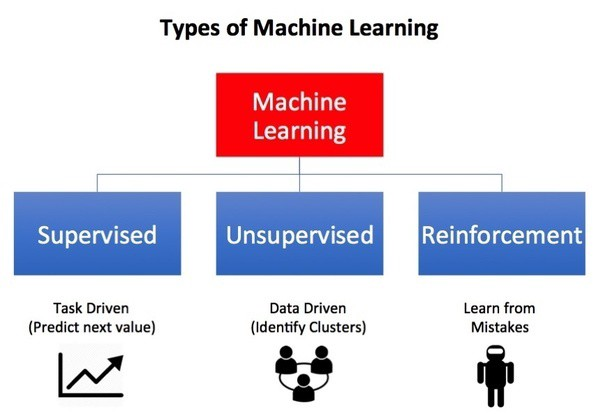
\includegraphics[width= 80mm]{types_of_ml.jpg}
\caption{\gr Είδη Μηχανικής Μάθησης \label{overflow}}
\end{figure}

Παραδείγματα αλγορίθμων επιβλεπόμενης μάθησης περιλαμβάνουν τους αλγόριθμους \en logistic regression, support vector machines \gr και τα νευρωνικά δίκτυα. Η μη επιβλεπόμενη μάθηση περιλαμβάνει την εκπαίδευση ενός μοντέλου σε δεδομένα χωρίς ετικέτες, αναζητώντας κρυφά πρότυπα ή εσωτερικές δομές. Παραδείγματα περιλαμβάνουν αλγόριθμους ομαδοποίησης όπως ο \en k-means\gr. Η ενισχυτική μάθηση είναι ένας τύπος μάθησης όπου ένας πράκτορας μαθαίνει να λαμβάνει αποφάσεις εκτελώντας ενέργειες σε ένα περιβάλλον για να μεγιστοποιήσει κάποια έννοια συνολικής ανταμοιβής.

Η μηχανική μάθηση έχει εφαρμοστεί επιτυχώς σε διάφορους τομείς όπως η υγειονομική περίθαλψη, η χρηματοοικονομική, το μάρκετινγκ και τα αυτόνομα συστήματα, δείχνοντας τη δυνατότητά της να μετασχηματίσει βιομηχανίες αυτοματοποιώντας πολύπλοκες εργασίες και παρέχοντας πολύτιμες πληροφορίες από δεδομένα \citep{goodfellow2016deep, bishop2006pattern}.

Η συνηθέστερη διαδικασία κατασκευής ενός μοντέλου μηχανικής μάθησης περιλαμβάνει τα εξής βασικά βήματα:
\begin{enumerate}
    \item \textbf{\gr Συλλογή Δεδομένων}
    \item \textbf{\gr Προεπεξεργασία Δεδομένων}
    \begin{itemize}
        \item \gr Κωδικοποίηση κατηγορηματικών χαρακτηριστικών (\textit{ \en Encoding Categorical Features})
        \begin{itemize}
            \item \en One-Hot Encoding \cite{yu2022missing}
            \item \en Label Encoding \cite{kosaraju2023categorical}
        \end{itemize}
    \end{itemize}
    \item \textbf{\gr Επιλογή Αλγορίθμου}
    \item \textbf{\gr Εκπαίδευση Μοντέλου} 
    \item \textbf{\gr Αξιολόγηση Μοντέλου}
\end{enumerate}

Κάθε βήμα είναι σημαντικό για τη δημιουργία ενός αποτελεσματικού μοντέλου που μπορεί να χρησιμοποιηθεί για προβλέψεις ή λήψη αποφάσεων.


\begin{figure}[ht!]
\centering
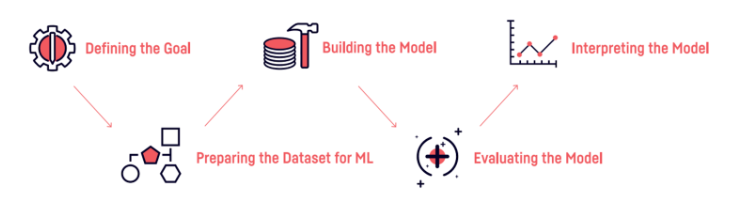
\includegraphics[width= 140mm]{ml_process.png}
\caption{\gr Διαδικασία εκπαίδευσης των Μοντέλων \label{overflow}}
\end{figure}
\subsection{\gr Προεπεξεργασία δεδομένων}

Η προεπεξεργασία δεδομένων αποτελεί θεμέλιο λίθο στη διαδικασία της μηχανικής μάθησης. Σαν ουσιαστικό βήμα, φροντίζει για την κατάλληλη προετοιμασία των δεδομένων, ώστε να τροφοδοτήσουν με ακρίβεια και αποτελεσματικότητα τα μοντέλα μηχανικής μάθησης, τόσο κατά την εκπαίδευση όσο και κατά την αξιολόγησή τους.

Σαν μια απαραίτητη διαδικασία, η προεπεξεργασία δεδομένων περιλαμβάνει ένα

Στη συνέχεια αναλύεται το εύρος εργασιών που εμπλέκονται στην προεπεξεργασία δεδομένων.

\subsubsection{\gr Καθαρισμός Δεδομένων}

Στόχος του καθαρισμού είναι ο εντοπισμός και η αντιμετώπιση τυχόν σφαλμάτων, ελλείψεων ή ασυνεπειών που δύναται να επηρεάσουν αρνητικά την εκπαίδευση και την απόδοση ενός μοντέλου.

\begin{itemize}
    \item \textbf{\gr Διαχείριση Ελλιπών Τιμών:} Οι ελλιπείς τιμές μπορούν να συμπληρωθούν χρησιμοποιώντας διάφορες τεχνικές όπως μέση τιμή, διάμεσος ή και να διαγραφούν αν η χρήση των παραπάνω τεχνικών δεν είναι ορθολογικά σωστη.
    \item \textbf{\gr Κανονικοποιήση Τιμών:} Οι ακραίες τιμές μπορούν να αφαιρεθούν ή να αναπροσαρμοστούν, δηλαδή να περιοριστούν σε ένα συγκεκριμένο όριο για να μειωθεί η επίδρασή τους στο μοντέλο.
    \item \textbf{\gr Εξαληψή Ασυνεπειών:} Οι ασυνέπειες στα δεδομένα, δηλαδή δεδομένα που δεν ακολουθούν την ίδια μορφοποίηση ή περιστάσεις όπου διαφορετικές πηγές δεδομένων δίνουν διαφορετικές τιμές για το ίδιο χαρακτηριστικό. Μπορούν να διορθωθούν ή να αφαιρεθούν για να εξασφαλιστεί η ομοιομορφία και η ακρίβεια.
\end{itemize}

\subsubsection{\gr Μετασχηματισμός Δεδομένων}

Αυτό το βήμα περιλαμβάνει τον μετασχηματισμό των δεδομένων σε μορφή κατάλληλη για τον επιλεγμένο αλγόριθμο μηχανικής μάθησης.

\begin{itemize}
    \item \textbf{Κλιμάκωση Αριθμητικών Χαρακτηριστικών:} Η κλιμάκωση διασφαλίζει ότι τα αριθμητικά χαρακτηριστικά έχουν συνεπή εμβέλεια, κάτι που είναι κρίσιμο για αλγορίθμους που είναι ευαίσθητοι στην κλίμακα των εισαγωγών δεδομένων.
    \item \textbf{\gr Κωδικοποίηση Κατηγορηματικών Χαρακτηριστικών:} Τα κατηγορικά χαρακτηριστικά μετατρέπονται σε αριθμητικές τιμές χρησιμοποιώντας τεχνικές όπως οι \en{one-hot encoding} \gr ή  \en{label encoding}\cite{analyticsvidhya2024}.
    \item \textbf{\gr Κατασκευή Χαρακτηριστικών:}\gr Νέα χαρακτηριστικά δημιουργούνται από τα υπάρχοντα για να παρέχουν πρόσθετες πληροφορίες στο μοντέλο.
\end{itemize}

\subsubsection{\gr Μείωση Δεδομένων}

Σε ορισμένες περιπτώσεις, τα σύνολα δεδομένων μπορεί να είναι πολύ μεγάλα και υπολογιστικά ακριβά για να δουλευτούν. Τεχνικές μείωσης δεδομένων όπως η μείωση διαστάσεων μπορούν να χρησιμοποιηθούν για να μειώσουν τον αριθμό των χαρακτηριστικών χωρίς να χαθεί σημαντική πληροφορία.

\begin{itemize}
    \item \textbf{Μείωση Διαστάσεων:} Τεχνικές όπως η Ανάλυση Κύριων Συνιστωσών (\en{Principal Component Analysis}\gr ή \en{PCA}) \gr ή η \en{t-Distributed Stochastic Neighbor Embedding} (\en{t-SNE}) \gr βοηθούν στη μείωση του αριθμού των χαρακτηριστικών διατηρώντας την ουσιώδη πληροφορία.
\end{itemize}

\subsubsection{\gr Οφέλη της Προεπεξεργασίας Δεδομένων}

\begin{itemize}
    \item \textbf{Βελτιωμένη Απόδοση Μοντέλου:} Τα προεπεξεργασμένα δεδομένα οδηγούν σε πιο ακριβή και αποδοτικά μοντέλα μηχανικής μάθησης.
    \item \textbf{Μειωμένος Χρόνος Εκπαίδευσης:} Τα καθαρά και οργανωμένα δεδομένα επιτρέπουν στα μοντέλα να εκπαιδεύονται πιο γρήγορα, βελτιστοποιώντας τους υπολογιστικούς πόρους.
    \item \textbf{Αυξημένη Ερμηνευσιμότητα Μοντέλου:} Η προεπεξεργασία βοηθά στον εντοπισμό σημαντικών χαρακτηριστικών και σχέσεων μέσα στα δεδομένα, κάνοντας το μοντέλο πιο εύκολο να ερμηνευτεί και να κατανοηθεί.
\end{itemize}

Εφαρμόζοντας με επιμέλεια αυτά τα βήματα προεπεξεργασίας δεδομένων, μπορούμε να βελτιώσουμε σημαντικά την ποιότητα του συνόλου δεδομένων μας, οδηγώντας σε καλύτερη απόδοση και αξιοπιστία των μοντέλων μηχανικής μάθησης. Κάθε βήμα παίζει ζωτικό ρόλο στην εξασφάλιση ότι τα δεδομένα είναι καθαρά, ενσωματωμένα, μετασχηματισμένα και μειωμένα κατάλληλα, θέτοντας μια στέρεη βάση για οποιοδήποτε έργο μηχανικής μάθησης.


\subsection{\gr Μόντελα μηχανικής Μάθησης}
Αυτή η ενότητα τα διαθέσιμα μοντέλα εποπτευόμενης μάθησης που μπορεί ο χρήστης να χρησιμοποιήσει μέσω του εργαλείου. Η εποπτευόμενη μάθηση, ένας ακρογωνιαίος λίθος της μηχανικής μάθησης, δίνει τη δυνατότητα στους αλγόριθμους να μαθαίνουν από δεδομένα που έχουν προεπισημανθεί με επιθυμητά αποτελέσματα. Αυτό επιτρέπει στα μοντέλα να εκτελούν ενέργειες όπως η ταξινόμηση  και η παλινδρόμηση. Θα εξετάσουμε τέσσερα σημαντικά μοντέλα εποπτευόμενης μάθησης: \en Logistic Regression, Random Forest, Support Vector Machine (SVM), and Naive Bayes.\gr Κάθε μοντέλο διαθέτει διακριτά χαρακτηριστικά και δείχνει αποτελεσματικότητα στην αντιμετώπιση διαφόρων τύπων προβλημάτων στο πλαίσιο αυτής της έρευνας.

\subsubsection{ \gr Λογιστική Παλινδρόμηση}
Αποτελεί θεμελιώδη αλγόριθμο εποπτευόμενης μάθησης που χρησιμοποιείται ευρέως για προβλήματα δυαδικής ταξινόμησης  \cite{hastie2009elements}. Εκτιμά την πιθανότητα ενός σημείου δεδομένων να ανήκει σε μια συγκεκριμένη κατηγορία (π.χ., η πιθανότητα έγκρισης ενός δανείου) \cite{taye2023understanding}.

\paragraph {\gr Ο αλγόριθμος }

Ο αλγόριθμος χρησιμοποιεί ένα γραμμικό μοντέλο παλινδρόμησης για την πρόβλεψη μιας συνεχούς τιμής μεταξύ αρνητικού άπειρου και θετικού άπειρου. Ωστόσο, για εργασίες ταξινόμησης, χρειαζόμαστε μια πιθανότητα μεταξύ 0 και 1. Για να το επιτύχουμε αυτό, η λογιστική παλινδρόμηση εφαρμόζει μια συνάρτηση \en{sigmoid} \gr(επίσης γνωστή ως λογιστική συνάρτηση) στην έξοδο του γραμμικού μοντέλου \cite{zaidi2023two}. Η συνάρτηση  \en{sigmoid}\gr  μετατρέπει την συνεχή έξοδο σε τιμή πιθανότητας.

\gr Ακολουθεί η μαθηματική αναπαράσταση του μοντέλου λογιστικής παλινδρόμησης:

\[
\en p(y = 1 | x) = \sigma(w^T x + b)
\]

\gr όπου:
\begin{itemize}
    \item \(p(y = 1 | x)\) \gr είναι η πιθανότητα της μεταβλητής στόχου \(y\) να είναι 1 δεδομένων των εισαγόμενων χαρακτηριστικών \(x\).
    \item \(\sigma\) \gr είναι η συνάρτηση \en sigmoid.
    \item \(w\) \gr είναι το διάνυσμα βαρών που αντιπροσωπεύει τους συντελεστές του γραμμικού μοντέλου.
    \item \(b\) \gr είναι ο όρος μετατόπισης.
    \item \(x\) \gr είναι το διάνυσμα των εισαγόμενων χαρακτηριστικών.
    \item \(w^T\) \gr δηλώνει το μετασχηματισμένο \en ( transposed) \gr διάνυσμα βαρών.
\end{itemize}

\gr Η συνάρτηση \en{sigmoid} ορίζεται ως:
\[
\sigma(z) = \frac{1}{1 + e^{-z}} 
\]
 \par {\gr όπου \(z = w^T x + b\). }

\gr Τα βήματα για την εκπαίδευση ενός μοντέλου λογιστικής παλινδρόμησης είναι τα εξής:

\begin{table}[h]
\centering
\caption{\gr Βήματα του Αλγορίθμου Λογιστικής Παλινδρόμησης}

\begin{tabular}{|l|p{10cm}|}
\hline
\textbf{\gr Βήμα} & \textbf{\gr Περιγραφή} \\ \hline
\gr Αρχικοποίηση & \gr Αρχικοποιούμε τα βάρη \(w\) και την μετατόπιση \(b\) σε μικρές τυχαίες τιμές. \\ \hline
\gr Προώθηση & \gr Υπολογίζουμε την προβλεπόμενη πιθανότητα \(\hat{y} = \sigma(w^T x + b)\) για κάθε παράδειγμα εκπαίδευσης. \\ \hline
\gr Υπολογισμός Απώλειας & \gr Υπολογίζουμε τη συνάρτηση απώλειας, συνήθως τη δυαδική διασταύρωση. \\ \hline
\gr Οπισθοπροώθηση & \gr Υπολογίζουμε τις κλίσεις της απώλειας σε σχέση με τα βάρη και τη μετατόπιση. \\ \hline
\gr Ενημέρωση Παραμέτρων & \gr Ενημερώνουμε τα βάρη και τη μετατόπιση χρησιμοποιώντας την καθοδική κλίση. \\ \hline
\gr Επανάληψη & \gr Επαναλαμβάνουμε τα βήματα 2-5 μέχρι να συγκλίνει το μοντέλο ή να φτάσει τον μέγιστο αριθμό επαναλήψεων. \\ \hline
\end{tabular}
\end{table}

\paragraph{\gr Κατάλληλες Εφαρμογές}

\gr Ο αλγοριθμος είναι θεωρείται κατάλληλος για εφαρμογές δυαδικής ταξινόμησης όπου η μεταβλητή εξόδου μπορεί να κατηγοριοποιηθεί σε δύο κατηγορίες. Εδώ είναι μερικά παραδείγματα:
\begin{itemize}
    \item \gr Ανίχνευση ανεπιθύμητων μηνυμάτων: Κατηγοριοποίηση των \en{emails} ως ανεπιθύμητα ή μη.
    \item \gr Πρόβλεψη εγκατάλειψης πελατών: Πρόβλεψη αν ένας πελάτης είναι πιθανό να σταματήσει να χρησιμοποιεί μια υπηρεσία.
    \item \gr Πρόβλεψη έγκρισης δανείου: Πρόβλεψη αν μια αίτηση δανείου θα εγκριθεί.
\end{itemize}

\paragraph{\gr Πλεονεκτήματα}

\begin{itemize}
    \item \textbf{\gr Ερμηνευσιμότητα:}  Οι συντελεστές του γραμμικού μοντέλου αντανακλούν άμεσα τη σημασία κάθε χαρακτηριστικού στην πρόβλεψη της μεταβλητής στόχου. Αυτό μας επιτρέπει να κατανοήσουμε πώς τα διάφορα χαρακτηριστικά συμβάλλουν στις προβλέψεις του μοντέλου.
    \item \textbf{\gr Απλότητα:}  Η λογιστική παλινδρόμηση είναι ένας σχετικά απλός αλγόριθμος που είναι εύκολο να υλοποιηθεί και να κατανοηθεί. Απαιτεί επίσης λιγότερη υπολογιστική ισχύ σε σύγκριση με ορισμένα άλλα μοντέλα.
    \item \textbf{\gr Αποτελεσματικότητα:} Η λογιστική παλινδρόμηση μπορεί να είναι πολύ αποτελεσματική για τη διαχείριση μεγάλων συνόλων δεδομένων.
\end{itemize}

\paragraph{\gr Τύποι Δεδομένων}

\gr Ο αλγόριθμος μπορεί να διαχειριστεί τόσο αριθμητικά όσο και κατηγορηματικά δεδομένα. Ωστόσο, τα κατηγορηματικά δεδομένα πρέπει να προεπεξεργαστούν σε αριθμητικά χαρακτηριστικά πριν την εισαγωγή τους στο μοντέλο. Αυτό μπορεί να γίνει με τεχνικές όπως η κωδικοποίηση \en{ one-hot}.

\paragraph{\gr Προεπεξεργασία}

\gr Εδώ είναι μερικά σημαντικά βήματα προεπεξεργασίας για τη λογιστική παλινδρόμηση:

\begin{itemize}
    \item \textbf{\gr Διαχείριση ελλειπόντων τιμών:} Οι ελλείπουσες τιμές μπορούν να συμπληρωθούν με τεχνικές όπως η συμπλήρωση με μέσο/διάμεσο ή να αφαιρεθούν αν το ποσοστό των ελλειπόντων δεδομένων είναι μικρό.
    \item \textbf{\gr Κλιμάκωση χαρακτηριστικών:}  Χαρακτηριστικά με διαφορετικές κλίμακες μπορούν να επηρεάσουν την απόδοση του μοντέλου. Η κλιμάκωση των χαρακτηριστικών σε ένα παρόμοιο εύρος μπορεί να βελτιώσει τη σύγκλιση του μοντέλου.
\end{itemize}

\paragraph{\gr Περιορισμοί}

\begin{itemize}
    \item \textbf{\gr Περιορισμένη σε δυαδική ταξινόμηση:}  Η λογιστική παλινδρόμηση μπορεί να διαχειριστεί μόνο εργασίες δυαδικής ταξινόμησης. Για προβλήματα πολλαπλών κατηγοριών, χρειάζονται άλλα μοντέλα όπως η πολυωνυμική λογιστική παλινδρόμηση ή η στρατηγική \en{ one-vs-rest.}
\end{itemize}

\subsubsection{\en Random Forest}
Το Δάσος Τυχαίων Δέντρων είναι ένας ευέλικτος αλγόριθμος εποπτευόμενης μάθησης που χρησιμοποιείται για εργασίες ταξινόμησης και παλινδρόμησης. Συνδυάζει πολλά δέντρα απόφασης για να βελτιώσει την ακρίβεια των προβλέψεων και να μειώσει τον κίνδυνο υπερεκπαίδευσης.

\paragraph{\gr Ο αλγόριθμος}

Ο αλγόριθμος Δάσους Τυχαίων Δέντρων δημιουργεί πολλαπλά δέντρα απόφασης από διαφορετικά υποσύνολα των δεδομένων εκπαίδευσης και στη συνέχεια συνδυάζει τις προβλέψεις τους \cite{rokach2016decision}. Η τελική πρόβλεψη γίνεται με ψηφοφορία για προβλήματα ταξινόμησης ή με τον μέσο όρο των προβλέψεων για προβλήματα παλινδρόμησης \cite{belgiu2016random}.

\begin{table}[h]
\centering
\caption{\gr Βήματα του Αλγορίθμου Δάσους Τυχαίων Δέντρων}
\begin{tabular}{|l|p{10cm}|}
\hline
\textbf{\gr Βήμα} & \textbf{\gr Περιγραφή} \\ \hline
\gr Επιλογή Υποσυνόλων & \gr Δημιουργήστε πολλαπλά υποσύνολα δεδομένων από το αρχικό σύνολο με επαναδειγματοληψία (\en bootstrapping)\gr. \\ \hline
\gr Δημιουργία Δέντρων Απόφασης & \gr Εκπαιδεύστε ένα δέντρο απόφασης σε κάθε υποσύνολο δεδομένων. \\ \hline
\gr Συνδυασμός Προβλέψεων & \gr Συνδυάστε τις προβλέψεις από όλα τα δέντρα για να δώσετε την τελική πρόβλεψη. \\ \hline
\end{tabular}
\end{table}

\paragraph{\gr Κατάλληλες Εφαρμογές}

\begin{itemize}
    \item \gr Αναγνώριση Μοτίβων: Κατηγοριοποίηση εικόνων και ήχων.
    \item \gr Ανίχνευση Απάτης: Πρόβλεψη απάτης σε συναλλαγές.
    \item \gr Πρόβλεψη Ασθενειών: Πρόβλεψη της πιθανότητας εμφάνισης ασθενειών από ιατρικά δεδομένα.
\end{itemize}

\paragraph{\gr Πλεονεκτήματα}

\begin{itemize}
    \item \textbf{\gr Ανθεκτικότητα στην Υπερεκπαίδευση:} Η χρήση πολλαπλών δέντρων μειώνει την πιθανότητα υπερεκπαίδευσης .
    \item \textbf{\gr Διαχείριση Ελλιπών Δεδομένων:} Τα δέντρα απόφασης μπορούν να διαχειριστούν ελλιπή δεδομένα, καθιστώντας το Δάσος Τυχαίων Δέντρων ανθεκτικό.
    \item \textbf{\gr Υψηλή Ακρίβεια:} Ο συνδυασμός πολλαπλών δέντρων συνήθως οδηγεί σε καλύτερη απόδοση σε σχέση με μεμονωμένα δέντρα \cite{breiman2022random}.
\end{itemize}


\paragraph{\gr Τύποι Δεδομένων}

Ο αλγόριθμος μπορεί να διαχειριστεί τόσο αριθμητικά όσο και κατηγορηματικά δεδομένα. Τα κατηγορηματικά δεδομένα μπορούν να κωδικοποιηθούν χρησιμοποιώντας τεχνικές όπως η κωδικοποιήσεις που έχουμε αναφέρει π.χ. \en{one-hot} \gr πριν την εισαγωγή τους στο μοντέλο \cite{goehry2023random}.

\paragraph{\gr Προεπεξεργασία}

\begin{itemize}
    \item \textbf{\gr Διαχείριση Ελλειπόντων Τιμών:} Οι ελλείπουσες τιμές μπορούν να συμπληρωθούν με τεχνικές όπως η συμπλήρωση με μέσο/διάμεσο ή να αφαιρεθούν εάν το ποσοστό των ελλειπόντων δεδομένων είναι μικρό.
    \item \textbf{\gr Κλιμάκωση Χαρακτηριστικών:} Παρόλο που το Δάσος Τυχαίων Δέντρων είναι λιγότερο ευαίσθητο σε χαρακτηριστικά με διαφορετικές κλίμακες, η κλιμάκωση των χαρακτηριστικών μπορεί να βελτιώσει την απόδοση του μοντέλου.\\
\end{itemize}


\paragraph{\gr Περιορισμοί}

\begin{itemize}
    \item \textbf{\gr Πολυπλοκότητα:} Το Δάσος Τυχαίων Δέντρων είναι πιο περίπλοκο και απαιτεί περισσότερους υπολογιστικούς πόρους από ένα μεμονωμένο δέντρο απόφασης.
    \item \textbf{\gr Μειωμένη Ερμηνευσιμότητα:} Η ερμηνεία του μοντέλου μπορεί να είναι πιο δύσκολη λόγω του μεγάλου αριθμού δέντρων που συνδυάζονται \cite.
\end{itemize}


\subsubsection{\en Support Vector Machine}
Η Υποστηρικτική Μηχανή Διανυσμάτων (\en{Support Vector Machine, SVM})\gr είναι ένας ισχυρός αλγόριθμος εποπτευόμενης μάθησης που χρησιμοποιείται για εργασίες ταξινόμησης και παλινδρόμησης. Ο \en{SVM} προσπαθεί να βρει το βέλτιστο υπερεπίπεδο που διαχωρίζει τις κατηγορίες των δεδομένων με τον μέγιστο περιθώριο.

\paragraph{\gr Ο αλγόριθμος}

Ο αλγόριθμος \en{SVM} \gr δημιουργήθηκε από τους \en Vapnik\gr και  \en Chervonenkis \gr και  λειτουργεί βρίσκοντας το υπερεπίπεδο που μεγιστοποιεί τον περιθώριο μεταξύ των διαφορετικών κατηγοριών \cite{hastie2017elements}. Το υπερεπίπεδο αυτό καθορίζεται από ένα μικρό υποσύνολο των δεδομένων εκπαίδευσης, τα οποία ονομάζονται διανύσματα υποστήριξης \cite{modhugu2024comparative}.

\begin{table}[h]
\centering
\caption{\gr Βήματα του Αλγορίθμου \en SVM \gr}
\begin{tabular}{|l|p{10cm}|}
\hline
\textbf{\gr Βήμα} & \textbf{\gr Περιγραφή} \\ \hline
\gr Επιλογή Χαρακτηριστικών & \gr Επιλέγουμε τα χαρακτηριστικά που θα χρησιμοποιηθούν για την εκπαίδευση του μοντέλου. \\ \hline
\gr Επιλογή Υποκειμένων & \gr Επιλέγουμε τα υποκείμενα δεδομένα που θα χρησιμοποιηθούν ως διανύσματα υποστήριξης. \\ \hline
\gr Βελτιστοποίηση Υπερεπιπέδου & \gr Υπολογίζουμε το υπερεπίπεδο που μεγιστοποιεί τον περιθώριο μεταξύ των κατηγοριών. \\ \hline
\end{tabular}
\end{table}

\paragraph{\gr Πλεονεκτήματα}

\begin{itemize}
    \item \textbf{\gr Υψηλή Ακρίβεια:} Προσφέρει υψηλή ακρίβεια στις προβλέψεις μεγιστοποιώντας το περιθώριο μεταξύ των δεδομένων. \cite{mohammadi2021comprehensive}.
    \item \textbf{\gr Αντοχή σε Υπερεκπαίδευση:} Ο \en{SVM} \gr έχει καλές ιδιότητες γενίκευσης, ιδιαίτερα σε μικρά σύνολα δεδομένων \cite{abdullah2021machine}.
    \item \textbf{\gr Ευελιξία:} Μπορεί να χρησιμοποιηθεί με διαφορετικούς πυρήνες (\en kernels)\gr για να προσαρμοστεί σε μη γραμμικά δεδομένα.
\end{itemize}

\paragraph{\gr Κατάλληλες Εφαρμογές}

\begin{itemize}
    \item \gr Αναγνώριση Προτύπων: Κατηγοριοποίηση εικόνων και αναγνώριση χειρογράφων.
    \item \gr Βιοπληροφορική: Ταξινόμηση βιολογικών δεδομένων και ανάλυση γονιδίων.
    \item \gr Ανίχνευση Απάτης: Πρόβλεψη και ανίχνευση απάτης σε συναλλαγές.
\end{itemize}

\paragraph{\gr Τύποι Δεδομένων}

Ο αλγόριθμος μπορεί να διαχειριστεί τόσο αριθμητικά όσο και κατηγορηματικά δεδομένα. Τα κατηγορηματικά δεδομένα πρέπει να μετατραπούν σε αριθμητικά πριν την εισαγωγή τους στο μοντέλο.

\paragraph{\gr Προεπεξεργασία}

Ακολουθούν μερικά σημαντικά βήματα προεπεξεργασίας για τον \en{SVM}:

\begin{itemize}
    \item \textbf{\gr Διαχείριση Ελλειπόντων Τιμών:} \gr Οι ελλείπουσες τιμές μπορούν να συμπληρωθούν ή να αφαιρεθούν από το σύνολο δεδομένων.
    \item \textbf{\gr Κλιμάκωση Χαρακτηριστικών:} Η κλιμάκωση των χαρακτηριστικών είναι σημαντική για την απόδοση του \en{SVM} \gr, καθώς επηρεάζει την απόδοση του μοντέλου.
\end{itemize}

\paragraph{\gr Περιορισμοί}

Αν και ο \en  SVM \gr αποτελεί έναν ισχυρό αλγόριθμο μηχανικής μάθησης με ευρεία εφαρμογή σε διάφορους τομείς. Η ικανότητά του να χειρίζεται τόσο γραμμικά όσο και μη γραμμικά δεδομένα, η υψηλή ακρίβεια και η ανθεκτικότητά του στην υπερεκπαίδευση το καθιστούν ένα πολύτιμο εργαλείο για την επίλυση προβλημάτων ταξινόμησης και παλινδρόμησης.
Ωστόσο:
\begin{itemize}
    \item \textbf{\gr Πολυπλοκότητα:} Μπορεί να είναι υπολογιστικά απαιτητικός, ιδιαίτερα με μεγάλα σύνολα δεδομένων.
    \item \textbf{\gr Δυσκολία Ερμηνείας:} Η ερμηνεία του μοντέλου μπορεί να είναι δύσκολη, ειδικά με μη γραμμικούς πυρήνες .
\end{itemize}

\subsubsection{\en Naive Bayes}
Ο \en{Naive Bayes} \gr είναι ένας αλγόριθμος εποπτευόμενης μάθησης που χρησιμοποιείται για εργασίες ταξινόμησης. Βασίζεται στον θεώρημα του \en Bayes \gr με την απλοποιημένη υπόθεση της ανεξαρτησίας μεταξύ των χαρακτηριστικών \cite{kaur2024wheat}.

\paragraph{\gr Ο αλγόριθμος}

Ο αλγόριθμος \en{Naive Bayes}\gr, βασισμένος στο θεώρημα Bayes, αποτελεί μια απλή αλλά ισχυρή μέθοδο ταξινόμησης δεδομένων. Η λειτουργία του βασίζεται στην υποθετική ανεξαρτησία των χαρακτηριστικών που περιγράφουν κάθε κατηγορία. Με απλά λόγια, υποθέτει πως η ύπαρξη μίας ιδιότητας σε μια κατηγορία δεν επηρεάζεται από την ύπαρξη άλλων ιδιοτήτων στην ίδια κατηγορία.\cite{narayan2021comparative}


\begin{table}[h]
\centering
\caption{\gr Βήματα του Αλγορίθμου\en Naive Bayes \gr}
\begin{tabular}{|l|p{10cm}|}
\hline
\textbf{\gr Βήμα} & \textbf{\gr Περιγραφή} \\ \hline
\gr Υπολογισμός Πιθανοτήτων & \gr Υπολογίζουμε τις πιθανότητες των διαφορετικών τάξεων. \\ \hline
\gr Υπολογισμός Συνθήκης Πιθανοτήτων & \gr Υπολογίζουμε τις συνθήκες πιθανότητες των χαρακτηριστικών δεδομένης της τάξης. \\ \hline
\gr Πρόβλεψη & \gr Χρησιμοποιούμε τις πιθανότητες για να προβλέψετε την τάξη ενός νέου δείγματος. \\ \hline
\end{tabular}
\end{table}

\paragraph{\gr Πλεονεκτήματα}

\begin{itemize}
    \item \textbf{\gr Απλότητα:} Είναι εύκολος στην κατανόηση και την υλοποίηση \cite{veziroglu2024performance,maswadi2021human}.
    \item \textbf{\gr Ταχύτητα:} Είναι γρήγορος και αποδοτικός, ιδιαίτερα για μεγάλα σύνολα δεδομένων \cite{ravinder2024web}.
    \item \textbf{\gr Χρήση με Μικρά Δεδομένα:} Μπορεί να έχει καλή απόδοση ακόμα και με μικρά σύνολα δεδομένων.
\end{itemize}

\paragraph{\gr Κατάλληλες Εφαρμογές}

\gr Ο \en{Naive Bayes} \gr είναι κατάλληλος για πολλές εφαρμογές όπως:
\begin{itemize}
    \item \gr Ανίχνευση Ανεπιθύμητων Μηνυμάτων: Ταξινόμηση emails ως ανεπιθύμητα ή μη.
    \item \gr Ανάλυση Συναισθήματος: Ταξινόμηση κειμένων με βάση το συναίσθημα που εκφράζουν.
    \item \gr Ιατρική Διάγνωση: Πρόβλεψη πιθανών ασθενειών με βάση τα συμπτώματα.
\end{itemize}

\paragraph{\gr Τύποι Δεδομένων}

Ο αλγόριθμος μπορεί να διαχειριστεί τόσο αριθμητικά όσο και κατηγορηματικά δεδομένα. Τα κατηγορηματικά δεδομένα μπορούν να μετατραπούν σε αριθμητικά πριν την εισαγωγή τους στο μοντέλο.

\paragraph{\gr Προεπεξεργασία}

Ακολουθούν μερικά σημαντικά βήματα προεπεξεργασίας για τον \en{Naive Bayes}:

\begin{itemize}
    \item \textbf{\gr Διαχείριση Ελλειπόντων Τιμών:} \gr Οι ελλείπουσες τιμές μπορούν να συμπληρωθούν ή να αφαιρεθούν από το σύνολο δεδομένων.
    \item \textbf{\gr Κλιμάκωση Χαρακτηριστικών:} \gr Η κλιμάκωση των χαρακτηριστικών μπορεί να βελτιώσει την απόδοση του μοντέλου, αν και ο \en{Naive Bayes} είναι λιγότερο ευαίσθητος στις διαφορές κλίμακας \cite{bishop2006pattern}.
\end{itemize}

\paragraph{\gr Περιορισμοί}

\begin{itemize}
    \item \textbf{\gr Απλοποιημένη Υπόθεση Ανεξαρτησίας:}\gr Ο αλγόριθμος υποθέτει ανεξαρτησία μεταξύ των χαρακτηριστικών, κάτι που σπάνια ισχύει στην πράξη.
    \item \textbf{\gr Ευαισθησία στις Σπάνιες Κατηγορίες:} Ο \en{Naive Bayes} \gr μπορεί να μην αποδίδει καλά όταν οι κατηγορίες έχουν πολύ λίγα δείγματα .
\end{itemize}

\subsection{\gr Μέθοδοι Αξιολόγησης Μοντέλου}

\gr Η αξιολόγηση αποτελεί θεμελιώδες κατά τη διαδικασία δημιουργία ενός μοντέλου μηχανικής μάθησης, καθώς μας επιτρέπει να ερμηνεύσουμε την απόδοση των μοντέλων και να επιλέξουμε το πλέον κατάλληλο για κάθε περίπτωση\cite{thakkar2022survey}.

\gr Πλήθος μετρικών έρχονται να φωτίσουν την αποτελεσματικότητα των μοντέλων, όπως:

\begin{itemize}
    \item \textbf{\gr Ακρίβεια (\en Accuracy\gr)}: \gr Η συχνότητα με την οποία το μοντέλο προβλέπει σωστά.
    \item \textbf{\gr Ανάκληση (\en Recall\gr)}: \gr Το ποσοστό των πραγματικά θετικών περιπτώσεων που ταυτοποιούνται σωστά.
    \item \textbf{\gr Ευστοχία (\en Precision\gr)}: \gr Το ποσοστό των αρνητικών περιπτώσεων που ταυτοποιούνται σωστά.
    \item \textbf{\en F1-score (\en F1 Score\gr)}: \gr Μέτρηση που συνδυάζει ακρίβεια και ανάκληση, προσφέροντας ισορροπημένη εικόνα.
\end{itemize}

\gr Αναλύοντας το μοντέλο βάσει των παραπάνω μετρικών οδηγούμαστε στην επιλογή του ιδανικού εργαλείου για το πρόβλημα που καλούμαστε να αντιμετωπίσουμε. Στη συνέχεια, αναλύονται αναλυτικότερα οι προαναφερθέντες μετρικές απόδοσης.


\subsubsection{\gr Ακρίβεια  (\en Accuracy\gr)}
\gr Η ακρίβεια είναι το ποσοστό των σωστών προβλέψεων προς τον συνολικό αριθμό των προβλέψεων. Είναι μια κοινή μετρική που χρησιμοποιείται όταν τα δεδομένα είναι ισορροπημένα, δηλαδή δεν υπάρχει σημαντική διαφορά στον αριθμό των παρατηρήσεων μεταξύ των διαφορετικών κατηγοριών \cite{powers2018evaluation}.

\subsubsection{\gr Ανάκληση (\en Recall)}
\gr Η ανάκληση, επίσης γνωστή ως ευαισθησία, μετρά την ικανότητα του μοντέλου να εντοπίζει με ακρίβεια τις θετικές περιπτώσεις. Είναι ιδιαίτερα χρήσιμη όταν είναι σημαντικό να μην χάνονται σημαντικά θετικά αποτελέσματα \cite{hancock2023evaluating}.\en
\[
\text{Recall} = \frac{\text{TP}}{\text{TP} + \text{FN}}
\]

\subsubsection{\gr Ευστοχία (\en Precision\gr)}

\gr Η ευστοχία (\en Precision \gr) είναι ένα από τα βασικά μέτρα αξιολόγησης της απόδοσης ενός ταξινομητή, ειδικά σε προβλήματα δυαδικής ταξινόμησης. Η ευστοχία ορίζεται ως το ποσοστό των σωστά προβλεπόμενων θετικών περιπτώσεων προς όλες τις περιπτώσεις που προβλέφθηκαν ως θετικές \cite{saranya2023comparative}.

\begin{equation}
\en Precision = \frac{\text{\en True Positives}}{\text{\en True Positives} + \text{\en False Positives}}
\end{equation}

\begin{figure}[ht!]
\centering
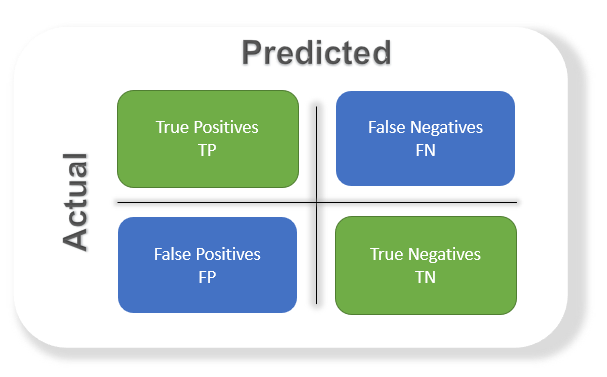
\includegraphics[width= 70mm]{confusion_matrix.png}
\caption{\gr Οπτική αναπαράσταση πινάκα σύγχυσης \label{overflow}}
\end{figure}

\gr όπου:
\begin{itemize}
    \item \(\text{\gr Αληθώς Θετικά (\en True Positives, TP \gr)}\): \gr Ο αριθμός των περιπτώσεων που ταξινομήθηκαν σωστά ως θετικές.
    \item \(\text{\gr Ψευδώς Θετικά (\en False Positives, FP \gr)}\): \gr Ο αριθμός των περιπτώσεων που ταξινομήθηκαν λανθασμένα ως θετικές.
\end{itemize}
\subsubsection{\en F1-Score}
\gr Το \en{F1-score} \gr είναι ο αρμονικός μέσος όρος της ακρίβειας και της ανάκλησης. Είναι χρήσιμο όταν υπάρχει ανισορροπία μεταξύ των κατηγοριών δεδομένων και επιθυμούμε ισορροπία μεταξύ ακρίβειας και ανάκλησης \cite{yacouby2020probabilistic}.\en
\[
\text{F1-Score} = 2 \cdot \frac{\text{Precision} \cdot \text{Recall}}{\text{Precision} + \text{Recall}}
\]

\subsection{\gr Μεροληψία στην Τεχνητή Νοημοσύνη}
\gr Η μεροληψία (\en bias \gr) στην τεχνητή νοημοσύνη (\en AI\gr) αποτελεί ένα από τα πλέον κρίσιμα ζητήματα, καθώς επηρεάζει άμεσα την αξιοπιστία και την ηθική χρήση των συστημάτων \en AI\gr. Με την αυξανόμενη χρήση των συστημάτων \en AI \gr σε τομείς όπως η υγειονομική περίθαλψη, η απασχόληση, η ποινική δικαιοσύνη και η πιστοληπτική αξιολόγηση, η ανησυχία για τη μεροληψία και την αμεροληψία των συστημάτων αυτών έχει ενταθεί.

\gr Οι πηγές της μεροληψίας είναι ποικίλες και περιλαμβάνουν τη συλλογή δεδομένων, το σχεδιασμό αλγορίθμων και τις ανθρώπινες αποφάσεις \cite{ferrara2023fairness}. Η μεροληψία μπορεί να οδηγήσει σε άδικα αποτελέσματα και να διαιωνίσει υπάρχουσες ανισότητες, καθώς τα μοντέλα \en AI \gr μπορεί να αναπαράγουν και να ενισχύουν κοινωνικά στερεότυπα.

\gr Οι αρνητικές επιπτώσεις της μεροληψίας επηρεάζουν τόσο τα άτομα όσο και την κοινωνία συνολικά. Για την αντιμετώπιση της μεροληψίας, έχουν προταθεί διάφορες στρατηγικές μετριασμού, όπως η βελτίωση της ποιότητας των δεδομένων, η επιλογή κατάλληλων μοντέλων και η επεξεργασία μετά την εκπαίδευση των μοντέλων.

\begin{figure}[ht!]
\centering
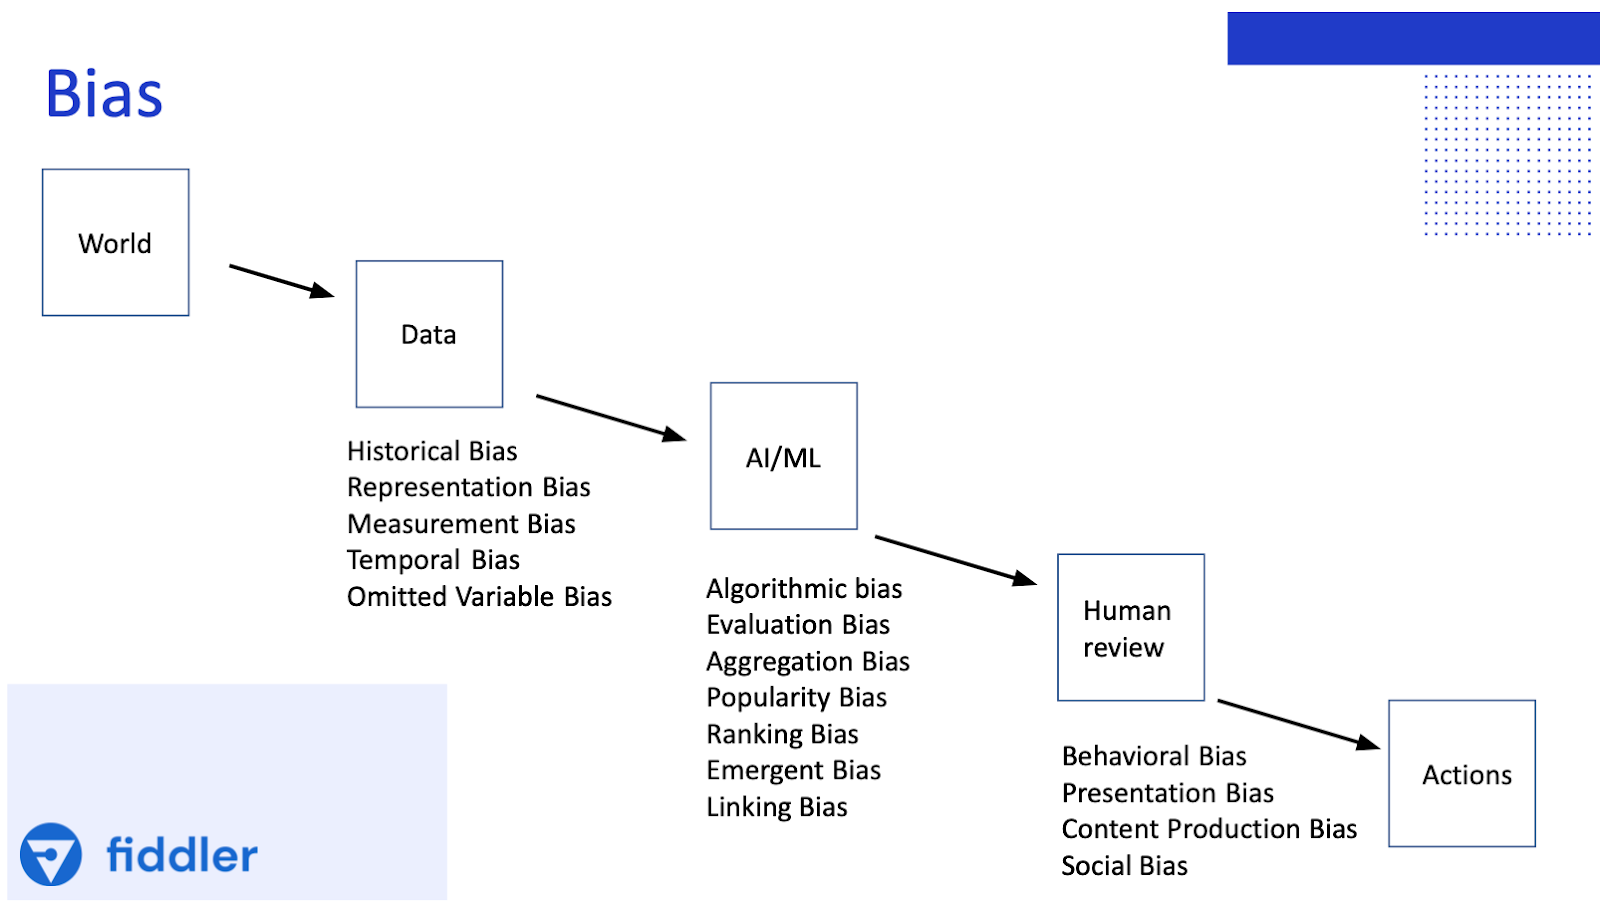
\includegraphics[width= 130mm]{bias_layers.png}f
\caption{\gr Σταδία πιθανής εμφάνισης Μεροληψίας  \label{overflow}}
\end{figure}

\gr Υπάρχουν διάφοροι τύποι μεροληψίας που μπορούν να επηρεάσουν τα μοντέλα \en machine learning\gr:

\begin{itemize}
 \item \textbf{\gr Μεροληψία Δεδομένων:} \gr
\begin{itemize}
    \item \textbf{\gr Μεροληψία Επιλογής (\en Sampling Bias ) :} \gr Εμφανίζεται όταν τα δεδομένα εκπαίδευσης δεν είναι αντιπροσωπευτικά του πληθυσμού στον οποίο θα εφαρμοστεί το μοντέλο. Για παράδειγμα, αν ένα σύστημα αναγνώρισης προσώπου εκπαιδευτεί κυρίως σε εικόνες ανοιχτόχρωμων ατόμων, μπορεί να έχει κακή απόδοση σε σκουρόχρωμα άτομα \citep{buolamwini2018gender}.
    \item \textbf{\gr Μεροληψία Μέτρησεων (\en Measurement  Bias) :} \gr Συμβαίνει όταν τα δεδομένα που συλλέγονται για εκπαίδευση ή αξιολόγηση περιέχουν ανακρίβειες ή συστηματικά λάθη. Για παράδειγμα, αν τα σφάλματα καταχώρισης δεδομένων είναι πιο συνηθισμένα για συγκεκριμένες δημογραφικές ομάδες, το μοντέλο μπορεί να μάθει να συνδέει αυτά τα λάθη με τις ίδιες τις ομάδες.
\end{itemize}
    \item \textbf{\gr Αλγοριθμική Μεροληψία:} \gr Αυτός ο τύπος μεροληψίας εμφανίζεται όταν το ίδιο το μοντέλο ή ο αλγόριθμος συμβάλλει σε μεροληπτικά αποτελέσματα. Για παράδειγμα, ορισμένοι αλγόριθμοι μπορεί να ευνοούν εγγενώς μια ομάδα έναντι άλλης αν δεν έχουν ρυθμιστεί σωστά ή αν ο σχεδιασμός τους δεν λαμβάνει υπόψη τις παραμέτρους δικαιοσύνης.
\end{itemize}

\gr Η κατανόηση και ο μετριασμός της μεροληψίας είναι κρίσιμης σημασίας, καθώς τα μεροληπτικά μοντέλα μπορούν να διαιωνίσουν και ακόμη και να ενισχύσουν τις υπάρχουσες ανισότητες, οδηγώντας σε σημαντικές συνέπειες σε κρίσιμους τομείς όπως οι προσλήψεις, η χορήγηση δανείων, η ποινική δικαιοσύνη και η υγειονομική περίθαλψη \citep{barocas2016big, o2016weapons}.

\subsection{\gr Αλγοριθμική μεροληψία και δικαιοσύνη στη μηχανική μάθηση}
Η αλγοριθμική μεροληψία αποτελεί ένα σημαντικό ζήτημα στη μηχανική μάθηση, καθώς τα μοντέλα που εκπαιδεύονται σε δεδομένα μπορεί να αντικατοπτρίζουν και να ενισχύουν υπάρχουσες προκαταλήψεις στην κοινωνία. Αυτό μπορεί να οδηγήσει σε άδικες και άνισες αποφάσεις που επηρεάζουν αρνητικά μειονοτικές ομάδες.

Για παράδειγμα, ένα μοντέλο που εκπαιδεύεται σε δεδομένα για την πρόβλεψη της εγκληματικότητας μπορεί να είναι πιο πιθανό να ταξινομήσει άτομα από μειονοτικές ομάδες ως πιθανούς εγκληματίες, ακόμα κι αν δεν έχουν παραβεί τον νόμο.

Η δικαιοσύνη στη μηχανική μάθηση εστιάζει στην ανάπτυξη αλγορίθμων που είναι δίκαιοι, αμερόληπτοι και δεν διακρίνουν εις βάρος συγκεκριμένων ομάδων. Αυτό περιλαμβάνει την αναγνώριση και την αντιμετώπιση πιθανών πηγών μεροληψίας στα δεδομένα εκπαίδευσης, τον σχεδιασμό αλγορίθμων που είναι ανθεκτικοί στη μεροληψία και την ανάπτυξη τεχνικών για την αξιολόγηση της δικαιοσύνης των μοντέλων μηχανικής μάθησης.

Είναι σημαντικό να λαμβάνουμε υπόψη την αλγοριθμική μεροληψία και να υιοθετούμε πρακτικές για την προώθηση της δικαιοσύνης στη μηχανική μάθηση, καθώς τα μοντέλα μηχανικής μάθησης ολοένα και περισσότερο επηρεάζουν τις ζωές μας.

\subsubsection{\gr Δικαιοσύνη στην τεχνητή νοημοσύνη}
\gr Η δικαιοσύνη στην τεχνητή νοημοσύνη περιλαμβάνει την εξασφάλιση ότι τα μοντέλα μηχανικής μάθησης αντιμετωπίζουν όλους τους ανθρώπους και τις ομάδες με δίκαιο τρόπο, χωρίς διακρίσεις ή προτιμήσεις. Υπάρχουν διάφοροι ορισμοί και μετρικές για τη δικαιοσύνη, που αντικατοπτρίζουν διαφορετικές προοπτικές και στόχους:

\begin{itemize}
    \item \textbf{\gr Δημογραφική Ισοτιμία:} \gr Ένα μοντέλο ικανοποιεί τη δημογραφική ισοτιμία αν η πιθανότητα ενός θετικού αποτελέσματος είναι η ίδια για διαφορετικές δημογραφικές ομάδες. Για παράδειγμα, ένας αλγόριθμος πρόσληψης θα πρέπει να επιλέγει υποψηφίους από διαφορετικές φυλετικές ομάδες με παρόμοια ποσοστά, υποθέτοντας ίσα προσόντα \citep{hardt2016equality}.
    \item \textbf{\gr Ισότητα Ευκαιριών:} \gr Αυτό το κριτήριο δικαιοσύνης απαιτεί τα άτομα σε διαφορετικές ομάδες που είναι εξίσου καταρτισμένα να έχουν ίσες πιθανότητες να επιλεγούν. Για παράδειγμα, ένα μοντέλο πιστωτικής αξιολόγησης θα πρέπει να εγκρίνει δάνεια για καταρτισμένους αιτούντες με ίσα ποσοστά ανεξάρτητα από το φύλο τους.
    \item \textbf{\gr Ισοτιμία Αποτελεσμάτων:} \gr Ένα μοντέλο ικανοποιεί την ισοτιμία αποτελεσμάτων αν έχει ίσα ποσοστά αληθινών θετικών και ψευδών θετικών για διαφορετικές δημογραφικές ομάδες. Αυτό σημαίνει ότι η ακρίβεια του μοντέλου είναι συνεπής μεταξύ των ομάδων, μειώνοντας την πιθανότητα δυσανάλογα υψηλών ψευδών θετικών ή ψευδών αρνητικών για οποιαδήποτε συγκεκριμένη ομάδα.
\end{itemize}

\gr Η επίτευξη δικαιοσύνης στα συστήματα τεχνητής νοημοσύνης είναι πρόκληση, καθώς διαφορετικές μετρικές δικαιοσύνης μπορεί να έρχονται σε σύγκρουση μεταξύ τους και η βελτιστοποίηση για μία μπορεί να οδηγήσει σε συμβιβασμούς σε μια άλλη. Επιπλέον, η δικαιοσύνη πρέπει να λαμβάνεται υπόψη στο πλαίσιο της συγκεκριμένης εφαρμογής και του κοινωνικού αντίκτυπου των αποφάσεων του μοντέλου \cite{chouldechova2020snapshot, stypinska2021ageism}.

\subsubsection{\gr Σημασία της αλγοριθμικής και Δικαιοσύνης στη μηχανική μάθηση}
\gr Η σημασία της αντιμετώπισης της αλγοριθμικής μεροληψίας και της εξασφάλισης δικαιοσύνης στη μηχανική μάθηση δεν μπορεί να υπερεκτιμηθεί. Τα μεροληπτικά μοντέλα μπορούν να οδηγήσουν σε άδικη μεταχείριση ατόμων, διαιωνίζοντας και ενισχύοντας τις κοινωνικές ανισότητες. Αυτό είναι ιδιαίτερα ανησυχητικό σε εφαρμογές υψηλού κινδύνου όπως η ποινική δικαιοσύνη, η υγειονομική περίθαλψη, η χρηματοοικονομική και η απασχόληση.\cite{pessach2023algorithmic,dolata2022sociotechnical}

\textbf{\gr Ποινική Δικαιοσύνη:} \gr Στο σύστημα ποινικής δικαιοσύνης, τα μεροληπτικά εργαλεία αξιολόγησης κινδύνου μπορούν να οδηγήσουν σε δυσανάλογα αυστηρές ποινές για τις μειονότητες. Μελέτες έχουν δείξει ότι ορισμένοι αλγόριθμοι που χρησιμοποιούνται για την πρόβλεψη των ποσοστών επανάληψης εγκλημάτων είναι μεροληπτικοί κατά των μαύρων κατηγορουμένων, οδηγώντας σε υψηλότερα ποσοστά ψευδών θετικών σε σύγκριση με τους λευκούς κατηγορούμενους \citep{angwin2022machine}.

\textbf{\gr Υγειονομική Περίθαλψη:} \gr Στην υγειονομική περίθαλψη, τα μεροληπτικά μοντέλα μπορούν να οδηγήσουν σε άνισα επίπεδα πρόσβασης στη θεραπεία και τη φροντίδα. Για παράδειγμα, ένα μοντέλο που εκπαιδεύτηκε κυρίως σε δεδομένα από άνδρες ασθενείς μπορεί να υποδιαγνώσει καταστάσεις που εμφανίζονται διαφορετικά σε γυναίκες ασθενείς, οδηγώντας σε υποβέλτιστη φροντίδα για τις γυναίκες \cite{obermeyer2019dissecting,chen2023algorithmic}.

\textbf{\gr Χρηματοοικονομική:} \gr Στον χρηματοοικονομικό τομέα, τα μεροληπτικά μοντέλα αξιολόγησης πιστοληπτικής ικανότητας μπορούν να αρνούνται δάνεια σε καταρτισμένους αιτούντες βάσει της φυλής ή της εθνικότητάς τους. Αυτή η διάκριση όχι μόνο επηρεάζει τις ευκαιρίες των ατόμων αλλά και διαιωνίζει τις οικονομικές ανισότητες \citep{bartlett2019consumer}.

\textbf{\gr Απασχόληση:} \gr Στις προσλήψεις, οι μεροληπτικοί αλγόριθμοι μπορούν να μειονεκτούν συγκεκριμένες δημογραφικές ομάδες, διαιωνίζοντας τις ανισότητες στο χώρο εργασίας. Για παράδειγμα, ένας αλγόριθμος πρόσληψης που εκπαιδεύτηκε σε βιογραφικά κυρίως από ένα φύλο ή μια φυλετική ομάδα μπορεί ακούσια να ευνοήσει υποψηφίους από αυτήν την ομάδα, υπονομεύοντας τις προσπάθειες για πολυμορφία και ένταξη \citep{raghavan2020mitigating}\\.

\gr Η αντιμετώπιση αυτών των ζητημάτων απαιτεί μια πολυδιάστατη προσέγγιση, συμπεριλαμβανομένης της ανάπτυξης και εφαρμογής μετρικών δικαιοσύνης, της χρήσης αλγορίθμων μετριασμού μεροληψίας και της καθιέρωσης νομικών και ηθικών κατευθυντήριων γραμμών. Εργαλεία όπως το \en IBM's AI Fairness 360 \gr που χρησιμοποιείται στην παρούσα εργασία αλλά και άλλες βιβλιοθήκες δικαιοσύνης οπως \en Fairlearn, VerifyML \gr κ.α. παρέχουν πρακτικές λύσεις για την ανίχνευση και τον μετριασμό της μεροληψίας, προσφέροντας μια σειρά από μετρικές και αλγορίθμους που μπορούν να ενσωματωθούν στη διαδικασία μηχανική μάθηση για την προώθηση της δικαιοσύνης \citep{hufthammer2020bias}.

\gr Επιπλέον, νομικά πλαίσια όπως το \en NYC Bias Audit Law of 2021, \gr που επιβάλλεται από το \en NYC Department of Consumer and Worker Protection (DCWP), \gr απαιτούν διαφάνεια και δικαιοσύνη στα αυτοματοποιημένα συστήματα απόφασης. Η συμμόρφωση με τέτοιους κανονισμούς εξασφαλίζει ότι οι οργανισμοί είναι υπεύθυνοι για τα αποτελέσματα των \en AI \gr συστημάτων τους και ότι τα άτομα προστατεύονται από τις διακριτικές πρακτικές.

\grΜε την κατανόηση και την αντιμετώπιση της αλγοριθμικής μεροληψίας, μπορούμε να κατασκευάσουμε πιο δίκαια , διαφανή και εξηγήσιμα συστήματα που μπορούν να εφαρμοστούν και να μην αδικούν κοινωνικές ομαδες.

\subsection{\gr Μετρικές Δικαιοσύνης}
\gr Οι μετρικές δικαιοσύνης \en(fairness metrics)\gr χρησιμοποιούνται για την αξιολόγηση και την εξασφάλιση της δικαιοσύνης στα μοντέλα μηχανικής μάθησης και τεχνητής νοημοσύνης. Είναι βασισμένες σε διάφορες θεωρητικές και πρακτικές αρχές που αποσκοπούν στην ποσοτικοποίηση της δικαιοσύνης και της μεροληψίας στα μοντέλα μηχανικής μάθησης. Αυτές οι αρχές προέρχονται από διάφορα επιστημονικά πεδία, όπως η στατιστική, η πληροφορική, η κοινωνιολογία και η νομική. Στη συνέχεια θα αναλύσουμε κάποιες από αυτές όπως η μέση διαφορά (\en{mean difference}), (\en{disparate impact}), η διαφορά ίσων ευκαιριών (\en{equal opportunity difference}), \gr η διαφορά μέσων όρων (\en{average odds difference}),\gr και ο δείκτης \en Theil ({Theil index}).

\subsubsection{\gr Μέση Διαφορά (\en Mean Difference)}
\gr Η μέση διαφορά μετρά τη διαφορά στην απόδοση του μοντέλου μεταξύ των διαφορετικών ομάδων. Υπολογίζεται ως η μέση διαφορά των προβλεπόμενων τιμών από τις πραγματικές τιμές ανά ομάδα. Χρησιμοποιείται συνήθως σε περιπτώσεις όπου θέλουμε να διασφαλίσουμε ότι οι προβλέψεις είναι ισορροπημένες μεταξύ διαφορετικών δημογραφικών ομάδων. Μια χαμηλή τιμή υποδεικνύει μεγαλύτερη δικαιοσύνη, καθώς σημαίνει ότι το μοντέλο προβλέπει με παρόμοια ακρίβεια για όλες τις ομάδες \cite{verma2018fairness}\en.
\[
\text{Mean Difference} = \frac{1}{n}\sum_{i=1}^{n} (\hat{y}_i - y_i)
\]

\begin{table}[h]
\centering
\caption{\en Mean Difference}
\begin{tabular}{|l|l|}
\hline
\textbf{\gr Όρος} & \textbf{\gr Περιγραφή} \\ \hline
\(\hat{y}_i\) & \gr Προβλεπόμενη τιμή για την παρατήρηση \(i\) \\ \hline
\(y_i\) & \gr Πραγματική τιμή για την παρατήρηση \(i\) \\ \hline
\(n\) & \gr Συνολικός αριθμός παρατηρήσεων \\ \hline
\end{tabular}
\end{table}

\subsubsection{\en Disparate Impact}
\gr Η μετρική υπολογίζει το λόγο των θετικών προβλέψεων που λαμβάνουν οι προστατευόμενες και οι μη προστατευόμενες ομάδες. Σκοπός της είναι να εντοπίσει τυχόν άνισες μεταχειρίσεις και διακρίσεις που ενδεχομένως υφίστανται οι προστατευόμενες ομάδες. Ένας λόγος κοντά στο 1 Υποδεικνύει ισότιμη μεταχείριση και δίκαιη διαδικασία. Όσο ο λογός των δύο ομάδων αποκλείνει από το 1, τότε αυτό αποτελεί άνισης μεταχείρισης των προστατευόμενες ομάδων \en.
\[
\text{\en Disparate Impact} = \frac{\text{Pr}(\hat{Y} = 1 | A = 0)}{\text{Pr}(\hat{Y} = 1 | A = 1)}
\]

\begin{table}[h]
\centering
\caption{\en Disparate Impact}
\begin{tabular}{|l|l|}
\hline
\textbf{\gr Όρος} & \textbf{\gr Περιγραφή} \\ \hline
\(\text{Pr}(\hat{Y} = 1 | A = 0)\) & \gr Πιθανότητα θετικής πρόβλεψης για μη προστατευμένη ομάδα \\ \hline
\(\text{Pr}(\hat{Y} = 1 | A = 1)\) & \gr Πιθανότητα θετικής πρόβλεψης για προστατευμένη ομάδα \\ \hline
\end{tabular}
\end{table}

\subsubsection{\gr Διαφορά Ίσων Ευκαιριών (\en Equal Opportunity Difference)}
\gr Η διαφορά ίσων ευκαιριών μετρά τη διαφορά στις ευαισθησίες (\en{true positive rates}) \gr μεταξύ των προστατευμένων και μη προστατευμένων ομάδων. Αυτή η μετρική είναι ιδιαίτερα χρήσιμη όταν θέλουμε να διασφαλίσουμε ότι το μοντέλο μας αντιμετωπίζει όλες τις ομάδες με τον ίδιο τρόπο όσον αφορά την αναγνώριση των θετικών περιπτώσεων \cite{lagioia2023algorithmic,bacchi2024same}.\en
\[
\text{Equal Opportunity Difference} = \text{TPR}_0 - \text{TPR}_1
\]

\begin{table}[h]
\centering
\caption{\en Equal Opportunity Difference}
\begin{tabular}{|l|l|}
\hline
\textbf{\gr Όρος} & \textbf{\gr Περιγραφή} \\ \hline
\(\text{TPR}_0\) & \gr Ευαισθησία (\en{true positive rate}) \gr για μη προστατευμένη ομάδα \\ \hline
\(\text{TPR}_1\) & \gr Ευαισθησία (\en{true positive rate}) \gr για προστατευμένη ομάδα \\ \hline
\end{tabular}
\end{table}

\subsubsection{\gr Διαφορά Μέσων Όρων (\en Average Odds Difference)}
\gr Η διαφορά μέσων όρων μετρά τη διαφορά στις ευαισθησίες και στις ειδικότητες (\en{true negative rates}) \gr μεταξύ των προστατευμένων και μη προστατευμένων ομάδων. Αυτή η μετρική είναι χρήσιμη για την αξιολόγηση της συνολικής απόδοσης του μοντέλου μεταξύ των ομάδων.\en
\[
\text{Average Odds Difference} = \frac{1}{2}[(\text{TPR}_0 - \text{TPR}_1) + (\text{TNR}_0 - \text{TNR}_1)]
\]

\begin{table}[h]
\centering
\caption{\en Average Odds Difference}
\begin{tabular}{|l|l|}
\hline
\textbf{\gr Όρος} & \textbf{\gr Περιγραφή} \\ \hline
\(\text{TPR}_0\) & \gr Ευαισθησία (\en{true positive rate}) \gr για μη προστατευμένη ομάδα \\ \hline
\(\text{TPR}_1\) & \gr Ευαισθησία (\en{true positive rate}) \gr για προστατευμένη ομάδα \\ \hline
\(\text{TNR}_0\) & \gr Ειδικότητα (\en{true negative rate}) \gr για μη προστατευμένη ομάδα \\ \hline
\(\text{TNR}_1\) & \gr Ειδικότητα (\en{true negative rate}) \gr για προστατευμένη ομάδα \\ \hline
\end{tabular}
\end{table}

\subsubsection{\gr Δείκτης \en Theil (Theil Index)}
\gr Ο δείκτης \en Theil \gr είναι ένα στατιστικό μέτρο οικονομικής ανισότητας που αναπτύχθηκε από τον οικονομολόγο \en Henri Theil. \gr Χρησιμοποιείται για την ποσοτικοποίηση των διαφορών στην κατανομή εισοδήματος ή πόρων μέσα σε έναν πληθυσμό. Είναι ιδιαίτερα χρήσιμος γιατί παρέχει μια σαφή, μαθηματική αναπαράσταση της ανισότητας, καθιστώντας το πολύτιμο εργαλείο που μπορεί να διακρίνει μεταξύ διαφορετικών πηγών ανισότητας, όπως η ανισότητα μεταξύ ομάδων και εντός ομάδων, που είναι χρήσιμο για τον εντοπισμό των συγκεκριμένων παραγόντων που συμβάλλουν στη συνολική ανισότητα \cite{dutt2021income, tizpaz2024how}.

\gr  Ο δείκτης \en Theil \gr δίνεται από\en: \\

\[
T = \frac{1}{N} \sum_{i=1}^N \left(\frac{y_i}{\overline{y}} \log \left( \frac{y_i}{\overline{y}} \right) \right)
\]

\gr όπου \( N \) είναι ο αριθμός των ατόμων, \( y_i \) είναι το εισόδημα του ατόμου \( i \), και \( \overline{y} \) είναι το μέσο εισόδημα. \en \\

\newpage

\begin{table}[h]
\centering
\caption{\gr Βήματα Υπολογισμού Δείκτη \en Theil (\en Theil Index Calculation Steps \gr)}
\begin{tabular}{|p{2cm}|p{12cm}|}
\hline
\textbf{\gr Βήμα} & \textbf{\gr Περιγραφή} \\ \hline
1. & \gr Προσδιορισμός Πληθυσμού. \en \\ \hline
2.  &\gr Συλλογή Δεδομένων Εισοδήματος. \en \\ \hline
3.  &\gr Υπολογισμός Συνολικού Εισοδήματος . \en \\ \hline
4.  &\gr Υπολογισμός Μέσου Εισοδήματος. \en \\ \hline
5. & \gr Υπολογισμός Αναλογίας Ατομικού Εισοδήματος . \en \\ \hline
6. & \gr Υπολογισμός Λογαρίθμου Αναλογιών κάθε ατόμου. \en \\ \hline
7. &\gr Υπολογισμός Σταθμισμένου Λογαρίθμου. \en \\ \hline
8. &\gr Άθροιση Σταθμισμένων Λογαρίθμων . \en \\ \hline
9. & \gr Υπολογισμός Δείκτη. \en \\
\hline
\end{tabular}
\end{table}

\newpage
\subsection{\gr Αλγόριθμοι Μείωσης Μεροληψίας}
\gr Η μείωση της μεροληψίας στα μοντέλα μηχανικής μάθησης είναι ζωτικής σημασίας για τη διασφάλιση της δικαιοσύνης και της ισότητας στις προβλέψεις. Οι αλγόριθμοι μείωσης μεροληψίας μπορούν να εφαρμοστούν σε τρία στάδια: προεπεξεργασία (\en pre-processing), \gr κατά την επεξεργασία (\en in-processing)\gr, και μετά την επεξεργασία (\en post-processing)\gr. Η επιλογή του κατάλληλου αλγορίθμου εξαρτάται από τη φύση των δεδομένων, το στάδιο της ανάπτυξης του μοντέλου, και τις συγκεκριμένες απαιτήσεις της εφαρμογής.

\begin{figure}[ht!]
\centering
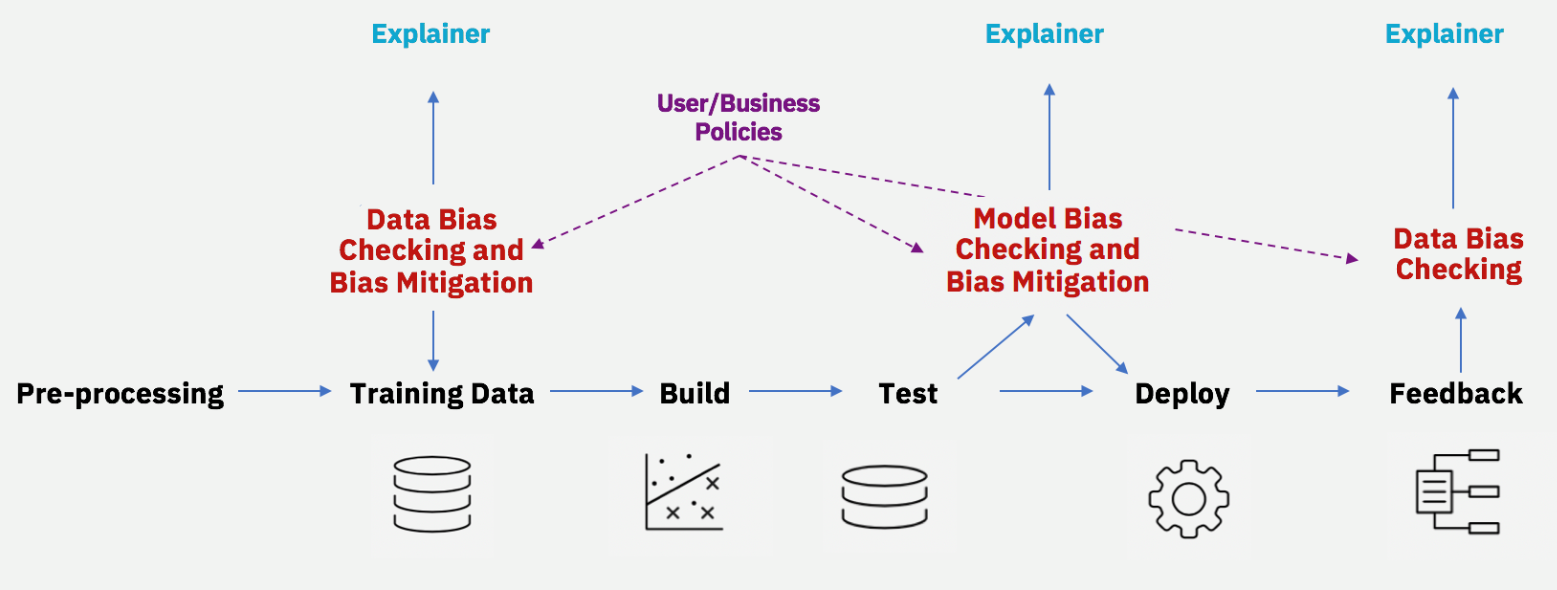
\includegraphics[width=120mm]{bias_mitigation.png}
\caption{\gr Στάδια Εφαρμογής των αλγόριθμων μείωσης μεροληψίας\label{overflow}}
\end{figure}

\begin{itemize}
 \item \textbf{ \en Pre-processing Algorithms: }\gr  Οι αλγόριθμοι προεπεξεργασίας αντιμετωπίζουν τη μεροληψία στα δεδομένα εκπαίδευσης πριν από την εκπαίδευση του μοντέλου. Αυτές οι μέθοδοι τροποποιούν το σύνολο δεδομένων έτσι ώστε οι προβλέψεις του μοντέλου να είναι πιο δίκαιες \cite{chen2023comprehensive}.
 \item \textbf{ \en In-Processing Algorithms : }\gr Αλγόριθμοι οι οποίοι εφαρμόζονται στο μοντέλο κατά τη διαδικασία της εκπαίδευσης του.
 \item \textbf{ \en Post-Processing Algorithms.: }\gr Οι αλγόριθμοι μετά την επεξεργασία εφαρμόζονται στις προβλέψεις του μοντέλου αφού το μοντέλο έχει ήδη εκπαιδευτεί. Αυτές οι τεχνικές τροποποιούν τις τελικές προβλέψεις για να βελτιώσουν τη δικαιοσύνη και δεν εμπλέκονται με κανένα από τα προηγούμενα στάδια.
\end{itemize}

\subsubsection{\gr Αναπροσαρμογή Βαρών (\en Reweighing)}
\grΗ τεχνική της αναπροσαρμογής των βαρών (\en{Reweighing}) χρησιμοποιείται στην προεπεξεργασία  (\en Pre-processing) \gr και περιλαμβάνει την αναπροσαρμογή των βαρών των παρατηρήσεων στο σύνολο δεδομένων εκπαίδευσης για να αντισταθμιστεί η μεροληψία. Αυτή η μέθοδος διασφαλίζει ότι οι προστατευμένες και μη προστατευμένες ομάδες έχουν παρόμοια επίδραση στην εκπαίδευση του μοντέλου \cite{feldman2015certifying}.\en
\[
\text{Weight}_{\text{new}} = \frac{\text{Total instances}}{\text{Instances of group}}
\]

\begin{table}[h]
\centering
\caption{\en Reweighing}
\begin{tabular}{|l|l|}
\hline
\textbf{\gr Όρος} & \textbf{\gr Περιγραφή} \\ \hline
\(\text{Weight}_{\text{new}}\) & \gr Νέο βάρος παρατήρησης \\ \hline
\(\text{Total instances}\) & \gr Συνολικός αριθμός παρατηρήσεων \\ \hline
\(\text{Instances of group}\) & \gr Αριθμός παρατηρήσεων της ομάδας \\ \hline
\end{tabular}
\end{table}

\subsubsection{\en Adversarial Debiasing}
\gr O αλγοριθμος (\en{Adversarial Debiasing}) \gr είναι μια μέθοδος κατά την επεξεργασία (\en In-processing) \gr που χρησιμοποιεί έναν αντίπαλο για να μειώσει τη μεροληψία στις προβλέψεις. Ο αλγόριθμος προσπαθεί να μεγιστοποιήσει την ακρίβεια των προβλέψεων ενώ ταυτόχρονα ελαχιστοποιεί τη δυνατότητα του αντιπάλου να προσδιορίσει τα προστατευόμενα χαρακτηριστικά \cite{yang2023adversarial}.\en
\[
\min \left( \text{Loss}_{\text{classifier}} - \lambda \cdot \text{Loss}_{\text{adversary}} \right)
\]

\begin{table}[h]
\centering
\caption{\en Adversarial Debiasing}
\begin{tabular}{|l|l|}
\hline
\textbf{\gr Όρος} & \textbf{\gr Περιγραφή} \\ \hline
\(\text{Loss}_{\text{classifier}}\) & \gr Συνάρτηση απώλειας ταξινομητή \\ \hline
\(\text{Loss}_{\text{adversary}}\) & \gr Συνάρτηση απώλειας αντιπάλου \\ \hline
\(\lambda\) & \gr Παράγοντας βαρύτητας \\ \hline
\end{tabular}
\end{table}

\subsubsection{\en Calibrated Equalized Odds}
\gr Ο αλγόριθμος (\en{Calibrated Equalized Odds}) \gr αποτελεί μέθοδο που εφαρμόζεται μετά την επεξεργασία  (\en Post-processing) \gr που χρησιμοποιεί την βαθμονόμηση των εξόδων του ταξινομητή για να βρει πιθανότητες με τις οποίες να αλλάξει τις ετικέτες εξόδου, διασφαλίζοντας ίσες πιθανότητες σφάλματος μεταξύ των ομάδων\en \cite{pleiss2017fairness}.
\[
\min \left( \text{Loss}_{\text{calibrated}} + \lambda \cdot \left( \left| \text{FPR}_{0} - \text{FPR}_{1} \right| + \left| \text{TPR}_{0} - \text{TPR}_{1} \right| \right) \right)
\]

\begin{table}[h]
\centering
\caption{\en Calibrated Equalized Odds}
\begin{tabular}{|l|l|}
\hline
\textbf{\gr Όρος} & \textbf{\gr Περιγραφή} \\ \hline
\(\text{Loss}_{\text{calibrated}}\) & \gr Συνάρτηση απώλειας βαθμονόμησης \\ \hline
\(\text{FPR}_{0}\) & \gr Ψευδώς θετικά ποσοστά για μη προστατευμένη ομάδα \\ \hline
\(\text{FPR}_{1}\) & \gr Ψευδώς θετικά ποσοστά για προστατευμένη ομάδα \\ \hline
\(\text{TPR}_{0}\) & \gr Πραγματικά θετικά ποσοστά για μη προστατευμένη ομάδα \\ \hline
\(\text{TPR}_{1}\) & \gr Πραγματικά θετικά ποσοστά για προστατευμένη ομάδα \\ \hline
\(\lambda\) & \gr Παράγοντας βαρύτητας \\ \hline
\end{tabular}
\end{table}

\section{\gr Νόμος για τον Έλεγχο Προκαταλήψεων του 2021}

\gr Ο σύγχρονος οργανωσιακός κόσμος υιοθετεί ολοένα και περισσότερο εργαλεία Τεχνητής Νοημοσύνης για βελτιστοποίηση των εσωτερικών διαδικασιών, συμπεριλαμβανομένων και των λειτουργιών Ανθρώπινου Δυναμικού. Η αξιοποίηση \en ΤΝ \gr για λήψη αποφάσεων πρόσληψης, απόλυσης ή προαγωγής φέρνει στο προσκήνιο εργασιακά ζητήματα και θέτει σε εφαρμογή νομοθεσίες περί ιδιωτικότητας, όπως ο Νόμος για τον Έλεγχο Προκαταλήψεων της Νέας Υόρκης, που επιβάλλει "Έλεγχο Αμεροληψίας" σε Αυτόματα Εργαλεία Λήψης Αποφάσεων Απασχόλησης (\en AEDT\gr) \cite{hilliard2023local}. Το παρόν κεφάλαιο εστιάζει στον  Νόμο για τον Έλεγχο Προκαταλήψεων \gr και τις απαιτήσεις του.

\subsection{\gr Ανάλυση Τοπικού  Νόμου  για τον Έλεγχο Προκαταλήψεων του 2021}
\gr Ο Νόμος για τον Έλεγχο Προκαταλήψεων του 2021, που εφαρμόστηκε από το Τμήμα Προστασίας Καταναλωτών και Εργαζομένων της Νέας Υόρκης (\en DCWP\gr) και είναι σε ισχύ από τον Ιανουάριο του έτους 2023, είναι μια πρωτοποριακή ρύθμιση με στόχο τη μείωση της μεροληψίας στα Αυτοματοποιημένα Εργαλεία Λήψης Αποφάσεων για Προσλήψεις (\en AEDTs\gr). Ο νόμος απαιτεί από τους εργοδότες και τις υπηρεσίες απασχόλησης να διενεργούν ετήσιους ελέγχους μεροληψίας στα \en AEDTs \gr και να δημοσιοποιούν αυτούς τους ελέγχους, εξασφαλίζοντας διαφάνεια και λογοδοσία στις πρακτικές προσλήψεων \cite{dcwp2024aedtp,dcwp2024faq}.

\subsection{\gr Μεροληψία Διασταυρούμενων Χαρακτηριστικών }
Ο κανόνας των τεσσάρων πέμπτων ( \en{four/fifths rule}\cite{watkins2022four} ) \gr είναι ένα σημαντικό εργαλείο για την αξιολόγηση της αλγοριθμικής δικαιοσύνης. Σύμφωνα με αυτόν τον κανόνα, μια συγκεκριμένη πρακτική θεωρείται ότι έχει \en{disparate impact}  \gr εάν το ποσοστό επιτυχίας μιας προστατευόμενης ομάδας είναι λιγότερο από το 80 τοις εκατό του ποσοστού επιτυχίας της ομάδας με την υψηλότερη επίδοση. Αυτή η μετρική χρησιμοποιείται για να αξιολογήσει αν υπάρχει ανισότητα στα αποτελέσματα μιας \en{αλγοριθμικής} απόφασης μεταξύ διαφορετικών ομάδων, όπως ορίζεται από τον \en{Title VII of the Civil Rights Act of 1964}. \gr Η μετρική \en{disparate impact} \gr επιτρέπει την αναγνώριση ανισοτήτων που δεν είναι άμεσα εμφανείς αλλά προκύπτουν από την εφαρμογή του \gr αλγόριθμου \cite{mack2023promoting,closedloop2023metric,islam2023differential}. 

Ωστόσο, αυτή η προσέγγιση δεν ήταν αρκετή για να διασφαλίσει την πλήρη δικαιοσύνη και αμεροληψία των αλγορίθμων. Με την ψήφιση του νόμου στη Νέα Υόρκη, εισήχθη η έννοια της διασταυρούμενων  (\en{intersectional}) \gr χαρακτηριστικών μεροληψίας, η οποία εξετάζει τα διάφορα χαρακτηριστικά των \en{datasets} \gr σε συνδυασμό και όχι μεμονωμένα. Αυτό σημαίνει ότι πρέπει να συνεχίζει να υπάρχει ο παραπάνω περιορισμός αλλά να εφαρμόζεται με βάση διασταυρούμενα χαρακτηριστικά (\en{intersectional attributes}) \gr. Ο νόμος αυτός επιδιώκει να εξαλείψει τη μεροληψία που μπορεί να προκύψει όταν ένας αλγόριθμος ευνοεί ή δυσχεραίνει ομάδες με βάση συνδυασμούς χαρακτηριστικών όπως το φύλο και η φυλή παραδείγματος χάρη. \cite{mcdonald2020intersectiona,subramanian2021evaluatingl}.

Η προσέγγιση αυτή αναγνωρίζει ότι οι άνθρωποι δεν ανήκουν μόνο σε μία κατηγορία (π.χ. φύλο ή φυλή), αλλά σε πολλές ταυτόχρονα, και ότι η δίκαιη αντιμετώπιση πρέπει να λαμβάνει υπόψη αυτές τις πολυπλοκότητες\cite{kong2022intersectionally}. 

\subsection{\gr Αντιμετώπιση της Διασταυρούμενης Μεροληψίας}
\gr Ο Νόμος για τον Έλεγχο Προκαταλήψεων εστιάζει στις ομάδες διασταυρούμενων χαρακτηριστικών, κάτι που είναι ιδιαίτερα κρίσιμο για την κατανόηση του πώς η μεροληψία μπορούν να επηρεάσουν δυσανάλογα τα άτομα που ανήκουν σε πολλαπλές περιθωριοποιημένες ομάδες. Τα παραδοσιακά μέτρα κατά των διακρίσεων συχνά αποτυγχάνουν να καταγράψουν τις σύνθετες μεροληψίες που αντιμετωπίζει, για παράδειγμα, μια μαύρη γυναίκα σε σύγκριση με έναν λευκό άνδρα. Οι διατάξεις του νόμου διασφαλίζουν ότι οι έλεγχοι μεροληψίας πρέπει να λαμβάνουν υπόψη διάφορες δημογραφικές ομάδες, συμπεριλαμβανομένων των διασταυρούμενων ταυτοτήτων, προωθώντας πιο δίκαιες πρακτικές προσλήψεων \cite{ulnicane2023power}.

\subsection{\gr Αξιοποίηση του Εργαλείου}
\gr Το εργαλείο το οποίο καλούμαστε να κατασκευάσουμε θα χρησιμοποιήσει κατά κόρον το \en AI Fairness 360 (AIF360) \gr είναι μια βιβλιοθήκη σχεδιασμένη για την ανίχνευση και μείωση της μεροληψίας στα μοντέλα μηχανικής μάθησης. Περιλαμβάνει εργαλεία για την αξιολόγηση της μεροληψίας σε διάφορες δημογραφικές ομάδες, παρέχοντας λεπτομερή ανάλυση που ευθυγραμμίζεται με τις απαιτήσεις του Νόμου  για τον Έλεγχο Προκαταλήψεων. Κάνοντας χρήση του \en AIF360,\gr οι οργανισμοί μπορούν να αξιολογούν τα \en AEDT \gr τους για μεροληψίες τόσο ενάντια σε προνομιούχες ομάδες (π.χ. λευκοί άνδρες) όσο και σε μη προνομιούχες ομάδες (π.χ. γυναίκες σκούρου δέρματος ) αποτελεσματικά \cite{wong2023seeing,lam2024framework}.

\subsection{\gr Πρακτική Εφαρμογή και Προκλήσεις}
\gr Παρόλο που το εργαλείο προσφέρει ισχυρές μετρικές για τον εντοπισμό μεροληψιών, υπάρχουν αρκετές πρακτικές προκλήσεις στην αποτελεσματική εφαρμογή αυτών των εργαλείων:

Απαιτήσεις Δεδομένων: Απαιτούνται λεπτομερή δημογραφικά δεδομένα, τα οποία μπορεί να είναι δύσκολο να αποκτηθούν και να επαληθευτούν. Ο Νόμος για τον Έλεγχο Προκαταλήψεων αντιμετωπίζει αυτό το ζήτημα απαιτώντας οι έλεγχοι μεροληψίας να αναφέρουν τον αριθμό των ατόμων που δεν παρείχαν δημογραφικά δεδομένα, εξασφαλίζοντας διαφάνεια στα δεδομένα που χρησιμοποιούνται για αυτούς τους ελέγχους \cite{iapp2023bias}.

Σύνθετα Μοντέλα: Η αποτελεσματικότητα του εργαλείου μπορεί να διαφέρει ανάλογα με την πολυπλοκότητα των \en AEDTs\gr. Είναι κρίσιμο να εξερευνηθούν σενάρια όπου το \en AIF360 \gr μπορεί να μην αποδίδει καλά, ιδιαίτερα σε μοντέλα με σύνθετες διαδικασίες λήψης αποφάσεων \cite{berente2021managing}.

Μεροληψία κατά το Σχεδιασμό:Η μεροληψία κατά τον σχεδιασμό και την εφαρμογή των \en AEDTs \gr μπορεί να παραμένουν. Ο αντιμετωπίζει έμμεσα αυτό το ζήτημα υπογραμμίζοντας την ανάγκη για εξωτερικούς ελέγχους, οι οποίοι μπορούν να παρέχουν αντικειμενική αξιολόγηση αυτών των εργαλείων \cite{uzougbo2024lega}.

\subsection{\gr Ενίσχυση της Διαφάνειας με την Επεξηγήσιμη Τεχνητή Νοημοσύνη}
\gr Η Καθηγήτρια \en Sarah Jones \gr από το \en MIT \gr υπογραμμίζει τη δυναμική της Επεξηγήσιμης Τεχνητής Νοημοσύνης (\en XAI\gr) να συμπληρώνει τα εργαλεία εντοπισμού μεροληψίας. Οι τεχνικές \en XAI \gr μπορούν να παρέχουν πληροφορίες για το πώς τα \en AEDTs \gr καταλήγουν στις αποφάσεις τους, καθιστώντας τη διαδικασία προσλήψεων πιο διαφανή τόσο για τους εργοδότες όσο και για τους υποψήφιους. Αυτή η διαφάνεια είναι ουσιώδης για την οικοδόμηση εμπιστοσύνης και την εξασφάλιση συμμόρφωσης με τον Nόμο για τον Έλεγχο Προκαταλήψεων της Νέας Υόρκης \cite{alam2023explainable}.

\subsection{\gr Συνεισφορά}
\gr Ο Νόμος για τον Έλεγχο Προκαταλήψεων μπορεί να λειτουργήσει ως πρότυπο για παρόμοιες ρυθμίσεις. Η έμφαση του στη διαφάνεια, τη διασταυρούμενη ανάλυση και τους τακτικούς ελέγχους θέτει υψηλά πρότυπα για δίκαιες πρακτικές προσλήψεων. Ωστόσο, η άμεση εφαρμογή αυτού του νόμου σε διαφορετικά πολιτιστικά πλαίσια μπορεί να αντιμετωπίσει προκλήσεις, όπως οι διαφορετικές ορισμοί της μεροληψίας και τα διαφορετικά ρυθμιστικά τοπία. Η εξερεύνηση αυτών των ευρύτερων επιπτώσεων μπορεί να παρέχει μια πιο ολοκληρωμένη κατανόηση του παγκόσμιου αντίκτυπού του \cite{osasona2024reviewing}. Η έμφαση του νόμου στους τακτικούς ελέγχους μεροληψίας και την λεπτομερή αναφορά δημογραφικών δεδομένων διασφαλίζει ότι οι αποχρώσεις των διασταυρούμενων μεροληψιών αντιμετωπίζονται, θέτοντας ένα προηγούμενο για μελλοντικές ρυθμίσεις στην Τεχνητή Νοημοσύνη και τις πρακτικές προσλήψεων \cite{balasubramaniam2023transparency}.
%%%%%%%%%%%%%%%%%%%%%%%%%%%%%%%%%%%%%%%%%%%%%%%%%%%%%%%
\newpage
\section{\gr Τεχνική Ανάλυση}
\gr Σε αυτό το κεφάλαιο, θα αναλύσουμε λεπτομερώς την αρχιτεκτονική και τη λειτουργικότητα του συστήματος που αναπτύξαμε. Θα παρουσιάσουμε το μοντέλο \en C4 \gr για την απεικόνιση της αρχιτεκτονικής του συστήματος, καθώς και διαγράμματα που αποτυπώνουν τις περιπτώσεις χρήσης, την ευρωστία, και τις ακολουθίες των διαδικασιών. Επιπλέον, θα αναλύσουμε τα εργαλεία και τις βιβλιοθήκες που χρησιμοποιήθηκαν και θα περιγράψουμε τη δομή των αρχείων κώδικα.

\subsection{Ανάλυση βάση του μοντέλου \en C4}
\gr Η ανάλυση της αρχιτεκτονικής του συστήματος βασίζεται στο μοντέλο \en C4 \gr, το οποίο δημιουργήθηκε από τον \en Simon Brown\gr. Το \en C4 \gr είναι μια μέθοδος απεικόνισης της διαδικασίας κατασκευής ενός συστήματος ή περιγραφής ενός ήδη υπάρχοντος συστήματος μέσω τεσσάρων επιπέδων: \en Context\gr, \en Container\gr, \en Component \gr, και \en Code \gr \cite{vazquez2020c4}. Τα διαγράμματα \en C4 \gr αποτελούν μια απλοποιημένη εναλλακτική λύση σε σύγκριση με τα διαγράμματα \en UML\gr, προσφέροντας δυνατότητα περιγραφής πολλαπλών συστημάτων \cite{thomas2023architectural}.

\begin{itemize}
    \item \textbf{Επίπεδο 1: \en Context} \\
\gr Το επίπεδο \en Context \gr παρέχει μια γενική εικόνα του συστήματος και των αλληλεπιδράσεών του με εξωτερικούς παράγοντες. Δείχνει το σύστημα που αναπτύσσεται, τους χρήστες του και τα άλλα συστήματα με τα οποία αλληλεπιδρά. Είναι το πιο αφαιρετικό επίπεδο και χρησιμεύει για την κατανόηση του περιβάλλοντος στο οποίο λειτουργεί το σύστημα.
    
\begin{figure}[h]
	\centering
	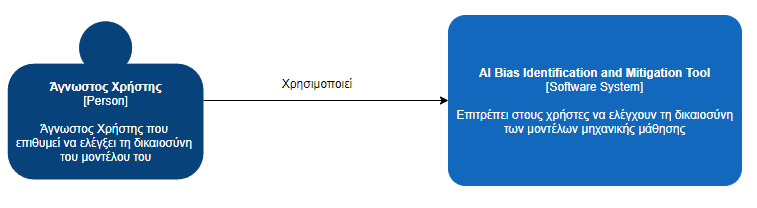
\includegraphics[width=80mm]{context_env.png}
	\caption{\gr Διάγραμμα Περιβάλλοντος συστήματος \label{overflow}}
\end{figure}

    \item \textbf{Επίπεδο 2: \en Container} \\
\gr Το επίπεδο \en Container \gr παρουσιάζει τη διάρθρωση του συστήματος σε επίπεδο \en container\gr, δηλαδή, τις κύριες εφαρμογές και υπηρεσίες που συνθέτουν το σύστημα. Περιγράφει τα \en container \gr και τον τρόπο με τον οποίο αυτά επικοινωνούν μεταξύ τους. 

\begin{figure}[h]
	\centering
	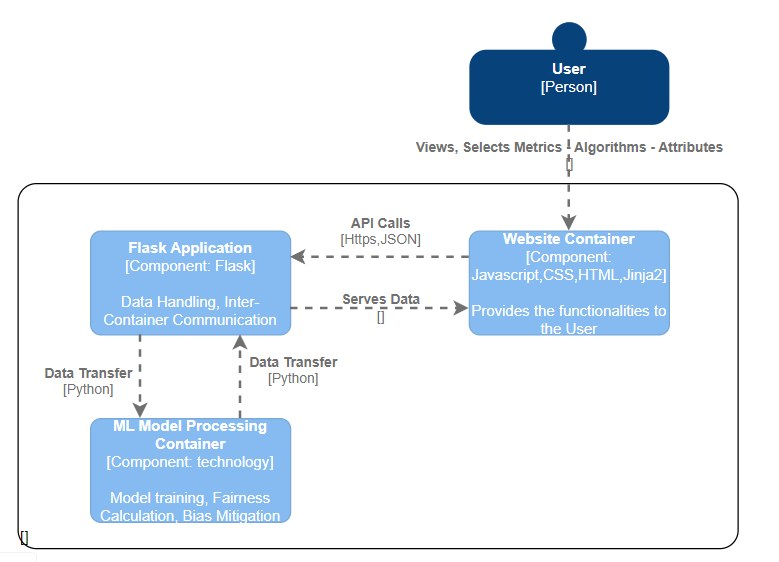
\includegraphics[width=120mm]{container_diagram.png}
	\caption{\en Container Diagram \gr του  συστήματος \label{overflow}}
\end{figure}

    \item \textbf{Επίπεδο 3: \en  Component} \\
\gr Το επίπεδο \en Component \gr προσφέρει μια λεπτομερή απεικόνιση των εσωτερικών συστατικών κάθε  \en container \gr και τον τρόπο με τον οποίο αυτά αλληλεπιδρούν μεταξύ τους. Εστιάζει στα επιμέρους τμήματα του λογισμικού μέσα σε κάθε  \en container \gr και τον τρόπο που αυτά συνδέονται και συνεργάζονται για να υλοποιήσουν τις λειτουργίες του συστήματος.
  
\newpage
\begin{figure}[h]
	\centering
	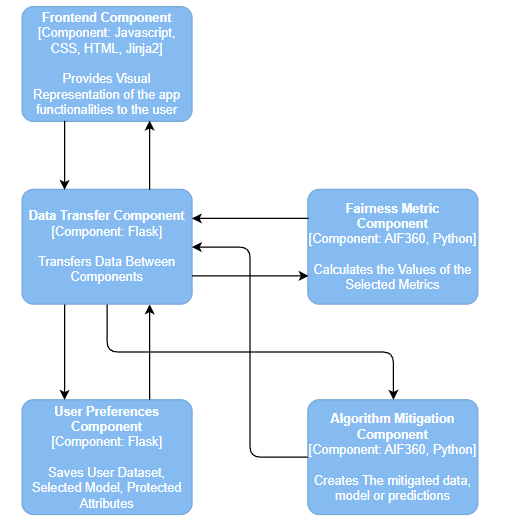
\includegraphics[width=120mm]{component_diagram.png}
	\caption{\en Component Diagram \gr του συστήματος \label{overflow}}
\end{figure}

    \item \textbf{Επίπεδο 4: \en  Code} \\
\gr Το επίπεδο \en Code \gr παρέχει την πιο λεπτομερή περιγραφή του συστήματος, εστιάζοντας στον πηγαίο κώδικα. Αυτό το επίπεδο αναλύει τη δομή του κώδικα, περιγράφοντας τις κλάσεις, τις μεθόδους και τις σχέσεις τους. Είναι χρήσιμο για τους προγραμματιστές που πρέπει να κατανοήσουν την ακριβή υλοποίηση και να συντηρήσουν το σύστημα.\en
\end{itemize}

\newpage
\begin{table}[h!]
\centering
\caption{\gr Αρχεία \en Python \gr και οι λειτουργίες τους}
\begin{tabular}{|l|p{10cm}|}
\hline
\textbf{\gr Όνομα Αρχείου} & \textbf{\gr Λειτουργίες} \\ \hline
\texttt{ \en app.py} & \gr Το κύριο αρχείο που διαχειρίζεται τις διαδρομές και τις βασικές λειτουργίες της εφαρμογής \en Flask\gr. Περιλαμβάνει τα \en routes \gr της εφαρμογής. \\ \hline
\texttt{ \en proccess.py} & \gr Περιέχει τις λειτουργίες επεξεργασίας των δεδομένων και εφαρμογής των αλγορίθμων μείωσης μεροληψίας. Διαχειρίζεται τη φόρτωση και προεπεξεργασία των \en dataset\gr, καθώς και την εφαρμογή των αλγορίθμων από την βιβλιοθήκη \en Aif360\gr. \\ \hline
\texttt{ \en examples.py} & \gr Περιέχει τη  λειτουργικότητα των παραδειγμάτων χρήσης και βοηθητικές λειτουργίες για την κατανόηση του τρόπου λειτουργίας του εργαλείου και την εκπαίδευση των χρηστών. \\ \hline
\end{tabular}
\end{table}

\newpage
\begin{table}[H]
\centering
\caption{\gr Συναρτήσεις του αρχείου \en proccess.py (Part 1)}
\begin{tabular}{|p{7cm}|p{7cm}|}
\hline
\textbf{\gr Συνάρτηση} & \textbf{\gr Περιγραφή} \\ \hline
\texttt{ \en prepare\_data} & \gr Προετοιμάζει τα δεδομένα για επεξεργασία. \\ \hline
\texttt{ \en process\_numerical\_variables} & \gr Επεξεργάζεται τις αριθμητικές μεταβλητές του \en dataset\gr. \\ \hline
\texttt{ \en encode\_categorical\_variables} & \gr Κωδικοποιεί τις κατηγορικές μεταβλητές του \en dataset\gr. \\ \hline
\texttt{ \en train\_model} & \gr Εκπαιδεύει το μοντέλο μηχανικής μάθησης. \\ \hline
\texttt{ \en calculate\_model\_metrics} & \gr Υπολογίζει τις επιλεγμένες μετρικές δικαιοσύνης. \\ \hline
\texttt{ \en convert\_to\_binary\_label\_dataset} & \gr Μετατρέπει το \en dataset \gr στην αντικείμενο της κλάσης \en binary dataset . \\ \hline
\texttt{ \en get\_binary\_datasets} & \gr Εξάγει δυαδικά \en datasets \gr από τα αρχικά δεδομένα. \\ \hline
\texttt{ \en calculate\_fairness\_metrics} & \gr Υπολογίζει τις μετρικές δικαιοσύνης. \\ \hline
\texttt{ \en get\_privildged\_group} & \gr Εντοπίζει την προνομιούχο ομάδα στο \en dataset \gr. \\ \hline
\texttt{ \en calculate\_standard\_metrics} & \gr Υπολογίζει μετρικές δικαιοσύνης για ομάδες βάση ενός χαρακτηριστικού. \\ \hline
\end{tabular}
\end{table}

\newpage
\begin{table}[H]
\centering
\caption{\gr Συναρτήσεις του αρχείου \en proccess.py (Part 2)}
\begin{tabular}{|p{7cm}|p{7cm}|}
\hline
\textbf{\gr Συνάρτηση} & \textbf{\gr Περιγραφή} \\ \hline
\texttt{ \en group\_results\_by\_metric} & \gr Ομαδοποιεί αποτελέσματα με βάση τη μετρική δικαιοσύνης. \\ \hline
\texttt{ \en fair\_check} & \gr Εκτελεί έλεγχο, αν το αποτέλεσμα της μετρικής δικαιοσύνης είναι εντός του ορισμένου \en threshold\gr. \\ \hline
\texttt{ \en train\_and\_evaluate} & \gr Εκπαιδεύει και αξιολογεί το μοντέλο. \\ \hline
\texttt{ \en mitigate} & \gr Μειώνει τη μεροληψία στο \en dataset \gr. \\ \hline
\texttt{ \en apply\_reweighing\_and\_train\_model} & \gr Εφαρμόζει τον αλγόριθμο \en Reweighing \gr και εκπαιδεύει το μοντέλο. \\ \hline
\texttt{ \en reweighing\_result} & \gr Παρέχει τα αποτελέσματα της τεχνικής \en Reweighing \gr. \\ \hline
\texttt{ \en apply\_adversarial\_debiasing\_\allowbreak and\_train\_model} & \gr Εφαρμόζει τον αλγόριθμο \en Adversarial Debiasing \gr και εκπαιδεύει το μοντέλο. \\ \hline
\texttt{ \en adversarial\_debiasing\_result} & \gr Παρέχει τα αποτελέσματα του αλγόριθμου \en Adversarial Debiasing \gr. \\ \hline
\texttt{ \en apply\_calibrated\_eq\_odds\_\allowbreak and\_train\_model} & \gr Εφαρμόζει τον αλγόριθμο \en Calibrated Equalized Odds \gr και εκπαιδεύει το μοντέλο. \\ \hline
\end{tabular}
\end{table}

\newpage
\begin{table}[H]
\centering
\caption{\gr Συναρτήσεις του αρχείου \en proccess.py (Part 3)}
\begin{tabular}{|p{7cm}|p{7cm}|}
\hline
\textbf{\gr Συνάρτηση} & \textbf{\gr Περιγραφή} \\ \hline
\texttt{ \en get\_reason} & \gr Παρέχει εξηγήσεις για τις αποφάσεις του μοντέλου. \\ \hline
\texttt{ \en construct\_metric\_info} & \gr Επιστρέφει πληροφορίες για τις μετρικές. \\ \hline
\texttt{ \en get\_ideal\_fairness\_value} & \gr Εντοπίζει την ιδανική τιμή δικαιοσύνης της μετρικής. \\ \hline
\texttt{ \en calibrated\_eq\_odds\_result} & \gr Παρέχει τα αποτελέσματα του αλγόριθμου \en Calibrated Equalized Odds \gr. \\ \hline
\texttt{ \en get\_mitigated\_results} & \gr Εξάγει τα αποτελέσματα μετά την εφαρμογή των τεχνικών μείωσης μεροληψίας. \\ \hline
\texttt{ \en wrap\_response} & \gr Επεξεργάζεται μορφοποιεί κατάλληλα το \en response \gr  για επεξεργασία απο το \en front-end. \\ \hline
\texttt{ \en calculate\_intersectional\_metrics} & \gr Υπολογίζει μετρικές  για ομάδες διασταυρούμενων χαρακτηριστικών. \\ \hline
\end{tabular}
\end{table}


\begin{table}[H]
\centering
\caption{\gr Συναρτήσεις του αρχείου \en examples.py}
\begin{tabular}{|l|p{10cm}|}
\hline
\textbf{\gr Συνάρτηση} & \textbf{\gr Περιγραφή} \\ \hline
\texttt{ \en create\_attsn\_value} & \gr Δημιουργεί χαρακτηριστικά και τιμές για παράδειγμα χρήσης. \\ \hline
\texttt{ \en get\_example\_dataset} & \gr Παρέχει \en dataset \gr για τα παραδείγματα της εφαρμογής. \\ \hline
\texttt{ \en get\_groups} & \gr Εξάγει τις ομάδες από το παράδειγμα που έχει επιλεχθεί. \\ \hline
\texttt{ \en get\_groups\_human\_readable} & \gr Παρέχει ομάδες σε αναγνώσιμη μορφή από τον άνθρωπο. \\ \hline
\texttt{ \en get\_example\_attributes} & \gr Εξάγει χαρακτηριστικά από το παράδειγμα από το παράδειγμα που έχει επιλεχθεί. \\ \hline
\texttt{ \en get\_data} & \gr Παρέχει τα δεδομένα για από το παράδειγμα που έχει επιλεχθεί. \\ \hline
\texttt{ \en get\_structured\_info} & \gr Παρέχει δομημένη πληροφορία για τα παραδείγματα. \\ \hline
\texttt{ \en train\_and\_evaluate} & \gr Εκπαιδεύει και αξιολογεί το μοντέλο παραδείγματος. \\ \hline
\texttt{ \en get\_mitigated\_results} & \gr Εξάγει τα αποτελέσματα μετά την εφαρμογή τεχνικών μείωσης μεροληψίας. \\ \hline
\texttt{ \en mitigate} & \gr Μειώνει τη μεροληψία από το παράδειγμα που έχει επιλεχθεί. \\ \hline
\end{tabular}
\end{table}

\newpage
\begin{table}[H]
\centering
\caption{\en HTML  \gr αρχεία και οι λειτουργίες τους}
\begin{tabular}{|l|p{10cm}|}
\hline
\textbf{\gr Όνομα Αρχείου} & \textbf{\gr Λειτουργίες} \\ \hline
\texttt{ \en base.html} & \gr Το κύριο πρότυπο που επεκτείνεται από τα υπόλοιπα αρχεία \en HTML\gr. \\ \hline
\texttt{ \en index.html} & \gr Η αρχική σελίδα της εφαρμογής. \\ \hline
\texttt{ \en chooseAtt.html} & \gr Σελίδα επιλογής προστατευόμενων χαρακτηριστικών για τον έλεγχο μεροληψίας. \\ \hline
\texttt{ \en metric.html} & \gr Σελίδα επιλογής μετρικών δικαιοσύνης. \\ \hline
\texttt{ \en fairness\_report.html} & \gr Σελίδα εμφάνισης των αποτελεσμάτων των μετρικών δικαιοσύνης. \\ \hline
\texttt{ \en algorithms.html} & \gr Σελίδα επιλογής αλγορίθμων μείωσης μεροληψίας. \\ \hline
\texttt{ \en example\_att.html} & \gr Σελίδα επιλογής χαρακτηριστικών των παραδειγματων. \\ \hline
\texttt{ \en mitigation\_report.html} & \gr Σελίδα παρουσίασης των αποτελεσμάτων μείωσης μεροληψίας. \\ \hline
\texttt{ \en selection.html} & \gr Σελίδα επιλογής και ανέβασμα dataset και μοντέλων μηχανικής μάθησης. \\ \hline
\end{tabular}
\end{table}

\newpage
\subsection{\gr Διάγραμμα Περιπτώσεων Χρήσης  }
Για να καθορίσουμε την απαιτούμενη λειτουργικότητα του συστήματος θα χρησιμοποιήσουμε διαγράμματα περίπτωσης χρήσης\cite{koc2021uml}, αναδεικνύοντας την αλληλεπίδραση του συστήματος με εξωτερικές οντότητες δηλαδή τους χρήστες και των λειτουργιών του συστήματος, τους παράγοντες, χωρίς όμως να γίνεται ανάλυση της δομής του, θα αναφερθούμε σε αυτό ως μαύρο κουτί. Στη συνέχεια θα παρουσιάσουμε τα διαγράμματα χρήσης:
\begin{enumerate}
\item «Χρήση \en Dataset \gr Χρήστη»
\item «Χρήση \en Demo Web Tool Dataset \gr »
\end{enumerate}
Θα ακολουθήσει οπτική και λεκτική ανάλυση των περιπτώσεων διαγραμμάτων χρήσης.
\begin{figure}[bp!]
\centering
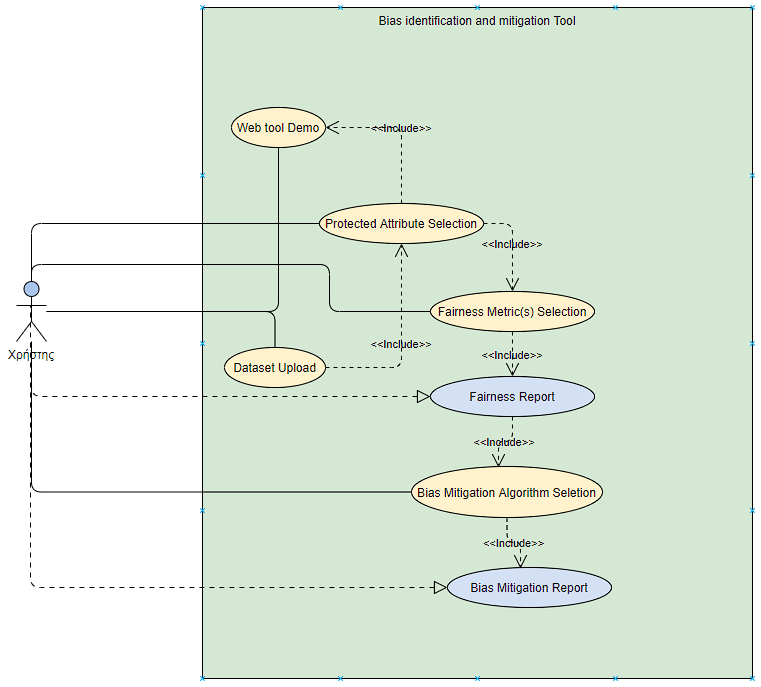
\includegraphics[width=110mm]{use_case.png}
\caption{\gr Διάγραμμα Περιπτώσεων Χρήσης \label{overflow}}
\end{figure}
\newpage
\begin{itemize}
\item \textbf{Περίπτωση Χρήσης 1:  «Χρήση \en Dataset \gr Χρήστη»  }
\newline\textbf{Αναγνωριστικό:} ΠΧ1
\newline\textbf{Περιγραφή:} Ο χρήστης επιλέγει να χρησιμοποιήσει \en dataset \gr της επιλογής του. Αφού πρώτα έχει ακολουθήσει τις οδηγίες για την τροποποίηση του \en dataset\gr.
\newline\textbf{Βασική Ροή:}
\begin{enumerate}
\item Ο χρήστης επιλέγει να ανεβάσει \en dataset \gr κατάλληλης μορφής και επιλέγει ένα αλγόριθμο με τον οποίο θα εκπαιδευτεί το μοντέλο του.
\item Το σύστημα μεταφέρει τον χρήστη στη σελίδα επιλογής προστατευόμενων χαρακτηριστικών.
\item Ο χρήστης επιλέγει τα προτεινόμενα προστατευόμενα χαρακτηριστικά και τις τιμές τους.
\item Το σύστημα μεταφέρει τον χρήστη στη σελίδα επιλογής μετρικών δικαιοσύνης.
\item Ο χρήστης επιλέγει όποιες από τις προτεινόμενες μετρικές δικαιοσύνης επιθυμεί.
\item Το σύστημα μεταφέρει τον χρήστη στη σελίδα αποτελεσμάτων των μετρικών δικαιοσύνης.
\item Ο χρήστης επιλέγει συνέχεια.
\item Το σύστημα μεταφέρει τον χρήστη στη σελίδα επιλογής αλγορίθμων μείωσης μεροληψίας.
\item Ο χρήστης επιλέγει οποιουσδήποτε αλγορίθμους μείωσης μεροληψίας επιθυμεί.
\item Το σύστημα μεταφέρει τον χρήστη στη σελίδα αποτελεσμάτων των μετρικών δικαιοσύνης όπου εφαρμόστηκαν οι αλγόριθμοι μείωσης μεροληψίας.
\end{enumerate}
\newpage
\textbf{Εναλλακτική Ροή:}
\begin{enumerate}
\item[1.α.1] Το σύστημα διαπιστώνει ότι το αρχείο του χρήστη είναι σε λάθος μορφή και εμφανίζει μήνυμα σφάλματος.
\item[6.α.1] Το σύστημα διαπιστώνει ότι το αρχείο του χρήστη είναι δίκαιο και εμφανίζει κατάλληλο μήνυμα.
\end{enumerate}
\item \textbf{Περίπτωση Χρήσης 2: «Χρήση \en Demo Web Tool Dataset \gr»  }
\newline\textbf{Αναγνωριστικό:} ΠΧ 2
\newline\textbf{Περιγραφή:} Ο χρήστης επιλέγει ένα από τα \en demo datasets \gr που προσφέρονται για την εκμάθηση χρήσης του εργαλείου στη σελίδα επιλογής.
\newline\textbf{Βασική Ροή:}
\begin{enumerate}
\item Ο χρήστης επιλέγει ένα από τα \en demo datasets \gr που προσφέρονται.
\item Το σύστημα μεταφέρει τον χρήστη στη σελίδα επιλογής προστατευόμενων χαρακτηριστικών.
\item Ο χρήστης επιλέγει τα προτεινόμενα προστατευόμενα χαρακτηριστικά και τις τιμές τους.
\item Το σύστημα μεταφέρει τον χρήστη στη σελίδα επιλογής μετρικών δικαιοσύνης.
\item Ο χρήστης επιλέγει όποιες από τις προτεινόμενες μετρικές δικαιοσύνης επιθυμεί.
\item Το σύστημα μεταφέρει τον χρήστη στη σελίδα αποτελεσμάτων των μετρικών δικαιοσύνης.
\item Ο χρήστης επιλέγει συνέχεια.
\item Το σύστημα μεταφέρει τον χρήστη στη σελίδα επιλογής αλγορίθμων μείωσης μεροληψίας.
\item Ο χρήστης επιλέγει οποιουσδήποτε αλγορίθμους μείωσης μεροληψίας επιθυμεί.
\item Το σύστημα μεταφέρει τον χρήστη στη σελίδα αποτελεσμάτων των μετρικών δικαιοσύνης όπου εφαρμόστηκαν οι αλγόριθμοι μείωσης μεροληψίας.
\end{enumerate}
\end{itemize}


\subsection{\gr Διάγραμματα Ευρωστίας  }

Τα διαγράμματα Ευρωστίας είναι η γραφική απεικόνιση των περιπτώσεων χρήσης του συστήματος ξεχωριστά. Στη συνέχεια παρατίθενται τα εν λόγω διαγράμματα.
\begin{figure}[H]
\centering
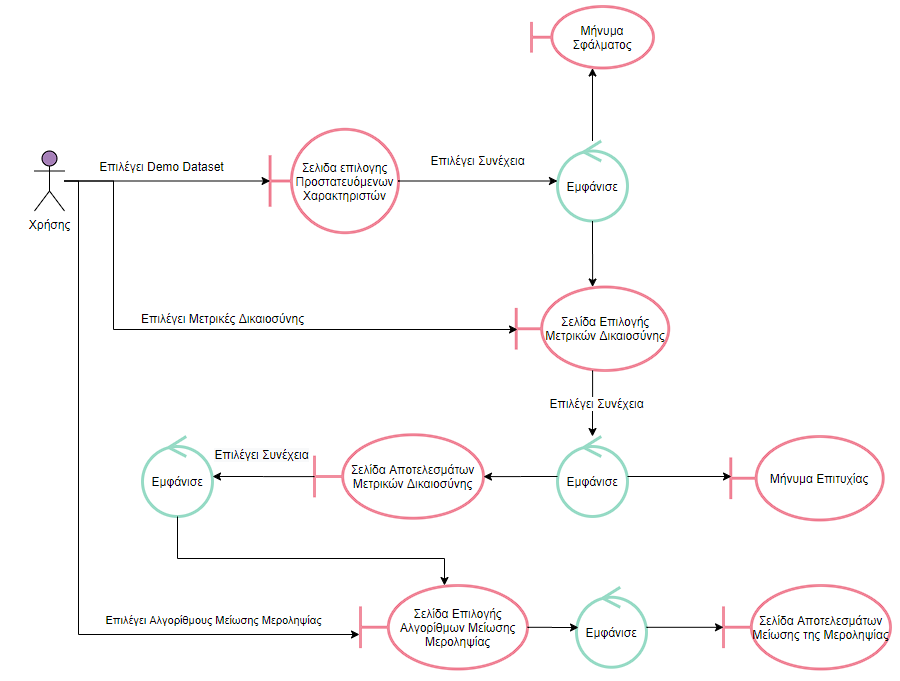
\includegraphics[width=140mm]{rob2.png}
\caption{\gr Διάγραμμα Ευρωστίας Περίπτωσης Χρήσης 1 \label{overflow}}
\end{figure}

\begin{figure}[bp!]
\centering
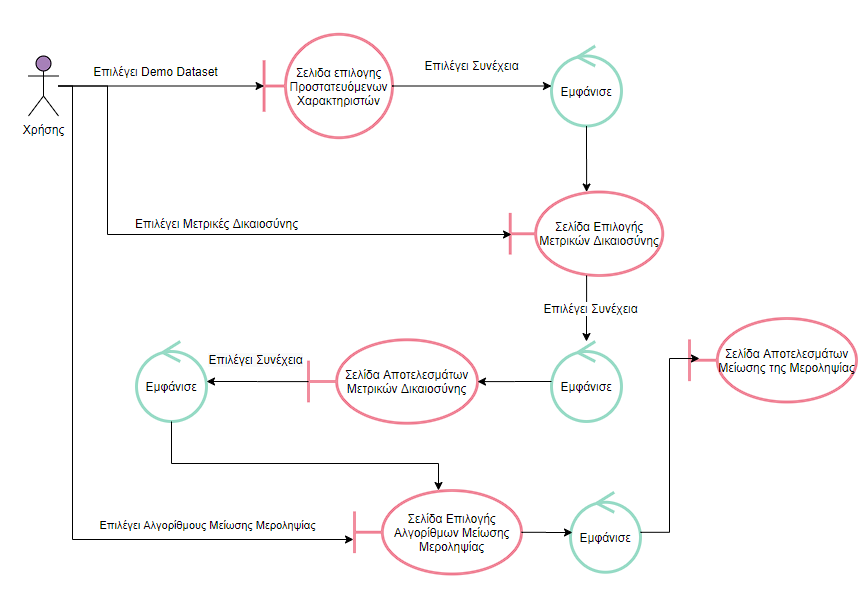
\includegraphics[width=140mm]{rob1.png}
\caption{\gr Διάγραμμα Ευρωστίας Περίπτωσης Χρήσης 2 \label{overflow}}
\end{figure}

\newpage
\subsection{\gr Διάγραμματα Ακολουθίας  }

Το διάγραμμα ακολουθίας απεικονίζει την αλληλεπίδραση μεταξύ αντικειμένων με διαδοχική σειρά, δηλαδή τη σειρά με την οποία πραγματοποιούνται αυτές οι αλληλεπιδράσεις. Ένα διάγραμμα ακολουθίας είναι δομημένο με τέτοιο τρόπο ώστε να αντιπροσωπεύει ένα χρονοδιάγραμμα που ξεκινά από την κορυφή και κατεβαίνει σταδιακά για να σημειώσει την ακολουθία των αλληλεπιδράσεων. Το διάγραμμα ακολουθίας ονομάζεται μερικές φορές διάγραμμα συμβάντων ή σενάριο συμβάντων. Παρακάτω ακολουθούν τα διαγράμματα ακολουθίας για κάθε περίπτωση χρήσης.

\begin{figure}[bp!]
\centering
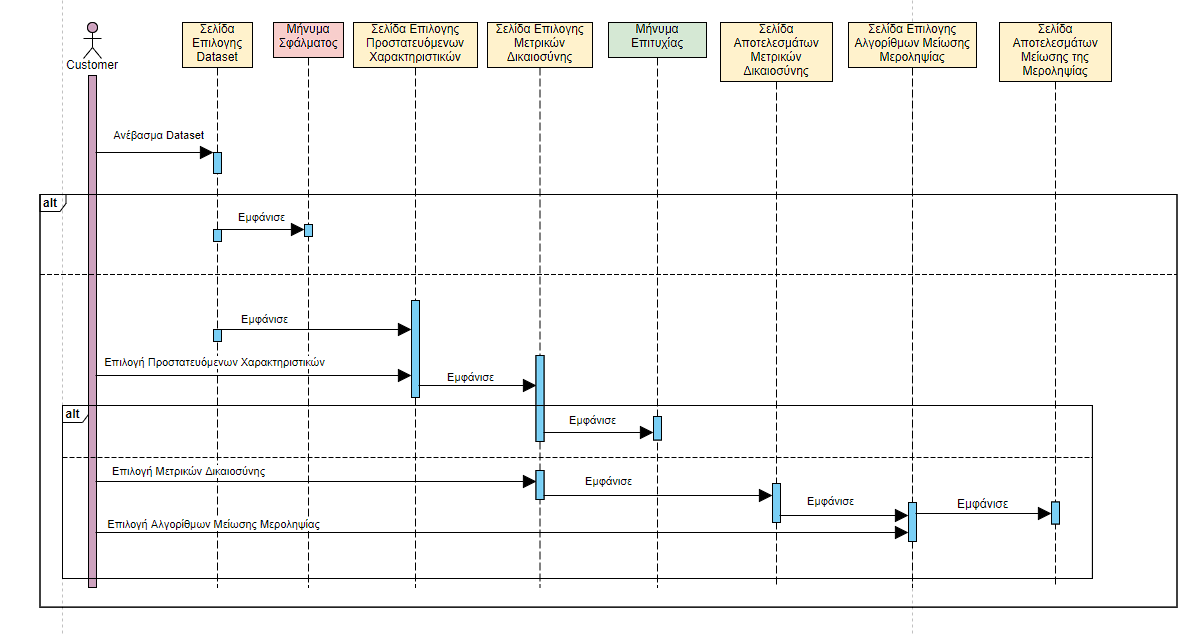
\includegraphics[width=170mm]{seq2.png}
\caption{\gr Διάγραμμα Ακολουθίας Περίπτωσης Χρήσης 1 \label{overflow}}
\end{figure}

\begin{figure}[H]
\centering
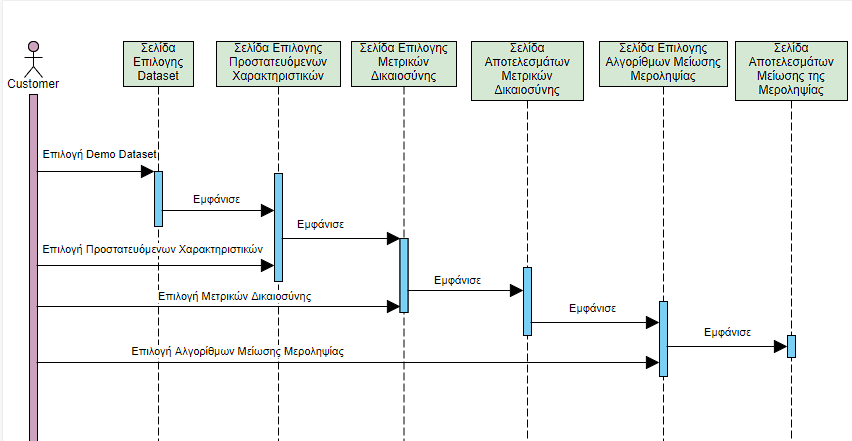
\includegraphics[width=170mm]{seq1.png}
\caption{\gr Διάγραμμα Ακολουθίας Περίπτωσης Χρήσης 2 \label{overflow}}
\end{figure}

\subsection{\gr Εργαλεία και Βιβλιοθήκες}
Στη συνέχεια παρουσιλαζονται τα διάφορα εργαλεία και βιβλιοθήκες που χρησιμοποιήθηκαν στην ανάπτυξη του συστήματός μας. Αυτές οι τεχνολογίες κατηγοριοποιήσαμε σε \en backend \gr και \en frontend \gr τεχνολογίες, περιγράφοντας τις λειτουργίες τους και τη σημασία τους.

\subsubsection{\en Backend \gr Τεχνολογίες}
\begin{itemize}
    \item \textbf{\en Flask \gr} - \en Flask \gr είναι ένα μικρό και επεκτάσιμο πλαίσιο για τη δημιουργία \en web \gr εφαρμογών σε \en Python \gr. Χρησιμοποιήθηκε για τη διαχείριση των διαδρομών και των βασικών λειτουργιών της εφαρμογής.
    
    \item \textbf{\en TensorFlow \gr} - Το  \en TensorFlow \gr είναι μια ανοιχτού κώδικα βιβλιοθήκη για μηχανική μάθηση και τεχνητή νοημοσύνη. Χρησιμοποιήθηκε για την ανάπτυξη και την εκπαίδευση των μοντέλων μηχανικής μάθησης \cite{singh2020introduction}.
    
    \item \textbf{\en AIF360 \gr} - Όπως έχει προαναφερθεί η \en AI Fairness 360 \gr είναι μια βιβλιοθήκη της \en IBM \gr που παρέχει αλγορίθμους και εργαλεία για τη μέτρηση και μείωση της μεροληψίας σε μοντέλα μηχανικής μάθησης\cite{zhang2021introduction} .
    
    \item \textbf{\en NumPy \gr} - Το \en NumPy \gr αποτελεί βιβλιοθήκη για την υποστήριξη μεγάλων, πολυδιάστατων πινάκων και συναρτήσεων μαθηματικών υπολογισμών σε \en Python \gr \cite{harris2020array}.
    
    \item \textbf{\en Scikit-learn \gr} - Το \en Scikit-learn \gr είναι μια βιβλιοθήκη μηχανικής μάθησης για τη γλώσσα προγραμματισμού \en Python \gr, που υποστηρίζει εποπτευόμενη και μη εποπτευόμενη μάθηση \cite{miranda2023hiclass,geron2022hands}.
    
    \item \textbf{\en Werkzeug \gr} - Το \en Werkzeug \gr είναι μια βιβλιοθήκη \en WSGI \gr για \en Python \gr που χρησιμοποιείται ως βοηθητικό εργαλείο για την ανάπτυξη \en web \gr εφαρμογών \cite{werkzeug2023}.
\end{itemize}

\subsubsection{\en Frontend \gr Τεχνολογίες}
\begin{itemize}
    \item \textbf{\en Bootstrap \gr 4.5.2} - \en Bootstrap \gr είναι ένα δημοφιλές πλαίσιο για τη δημιουργία αντιδραστικών και κινητών πρώτων \en web \gr ιστοσελίδων. Χρησιμοποιήθηκε για τη σχεδίαση του \en frontend \gr της εφαρμογής.
    
    \item \textbf{\en jQuery \gr} - \en jQuery \gr είναι μια γρήγορη, μικρή και πλούσια σε χαρακτηριστικά βιβλιοθήκη \en JavaScript \gr. Χρησιμοποιήθηκε για τη διευκόλυνση της γραφής σεναρίων \en HTML \gr.
    
    \item \textbf{\en Chart.js \gr} - \en Chart.js \gr είναι μια απλή αλλά ευέλικτη βιβλιοθήκη \en JavaScript \gr για την κατασκευή γραφημάτων. Χρησιμοποιήθηκε για την γραφική απεικόνιση των αποτελεσμάτων\cite{benbba2021comparison} .
    
    \item \textbf{\en D3.js \gr} - \en D3.js \gr είναι μια βιβλιοθήκη \en JavaScript \gr για την παραγωγή δυναμικών, διαδραστικών απεικονίσεων δεδομένων στο \en web \gr . Χρησιμοποιήθηκε για την κατασκευή βοηθήματος του χρήστη για την επιλογή κατάλληλων μετρικών\cite{rothenhausler2022d3}.
\end{itemize}

\newpage
%%%%%%%%%%%%%%%%%%%%%%%%%%%%%%%%%%%%%%%%%%%%%%%%%%%%%%%
\section{Παρουσίαση Εργαλείου και  Εκπαιδευτικής Διαδικασίας}
Στο κεφαλαίο αυτό θα αναλύσουμε την περίπτωση κατά την οποία ένας χρήστης επιθυμεί να εξοικειωθεί με το εργαλείο επιλέγοντας την εκπαιδευτική λειτουργία του εργαλείου, μέσω των διαθέσιμων \en demo dataset \gr  της εφαρμογής.

\subsection{Αρχική Σελίδα}

Πρόκειται για τη σελίδα υποδοχής του εργαλείου, στην οποία καλωσορίζεται ο χρήστης και του γίνεται μια σύντομη περιγραφή της λειτουργικότητας της εφαρμογής.

\begin{figure}[H]
\centering
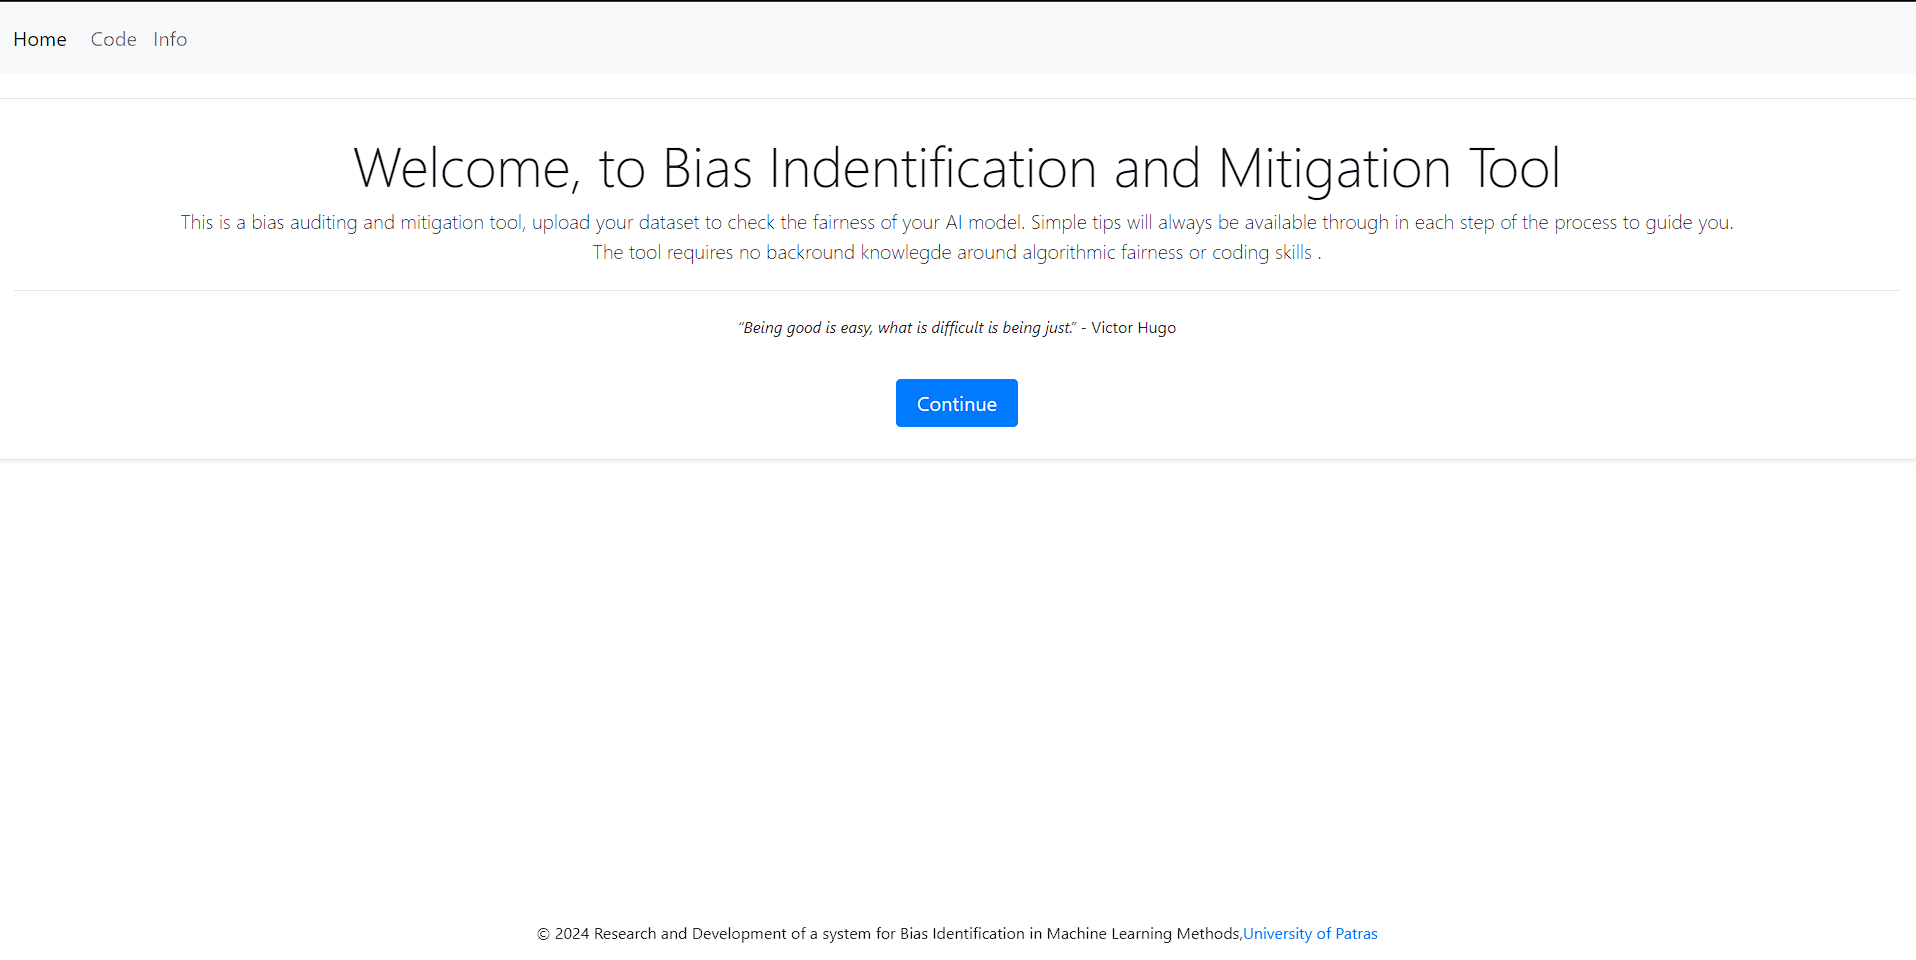
\includegraphics[width=150mm]{index_page.png}
\caption{\gr  Σελίδα υποδοχής της εφαρμογής \label{overflow}}
\end{figure}

\subsection{Επιλογή Συνόλου Δεδομένων}

\textit{Υποθετικό Σενάριο:} Ο χρήστης επιλέγει το σύνολο δεδομένων \en Compass Recidivism Risk Assessment\cite{hutchinson2023compass}, \gr το οποίο περιέχει μεταβλητές που χρησιμοποιούνται από τον αλγόριθμο \en COMPAS \gr  για την αξιολόγηση κατηγορουμένων. Η βαθμολογία αυτή αξιοποιείται από δικαστές και αξιωματούχους για την εκτίμηση της πιθανότητας υποτροπής των κατηγορουμένων.

\begin{figure}[H]
\centering
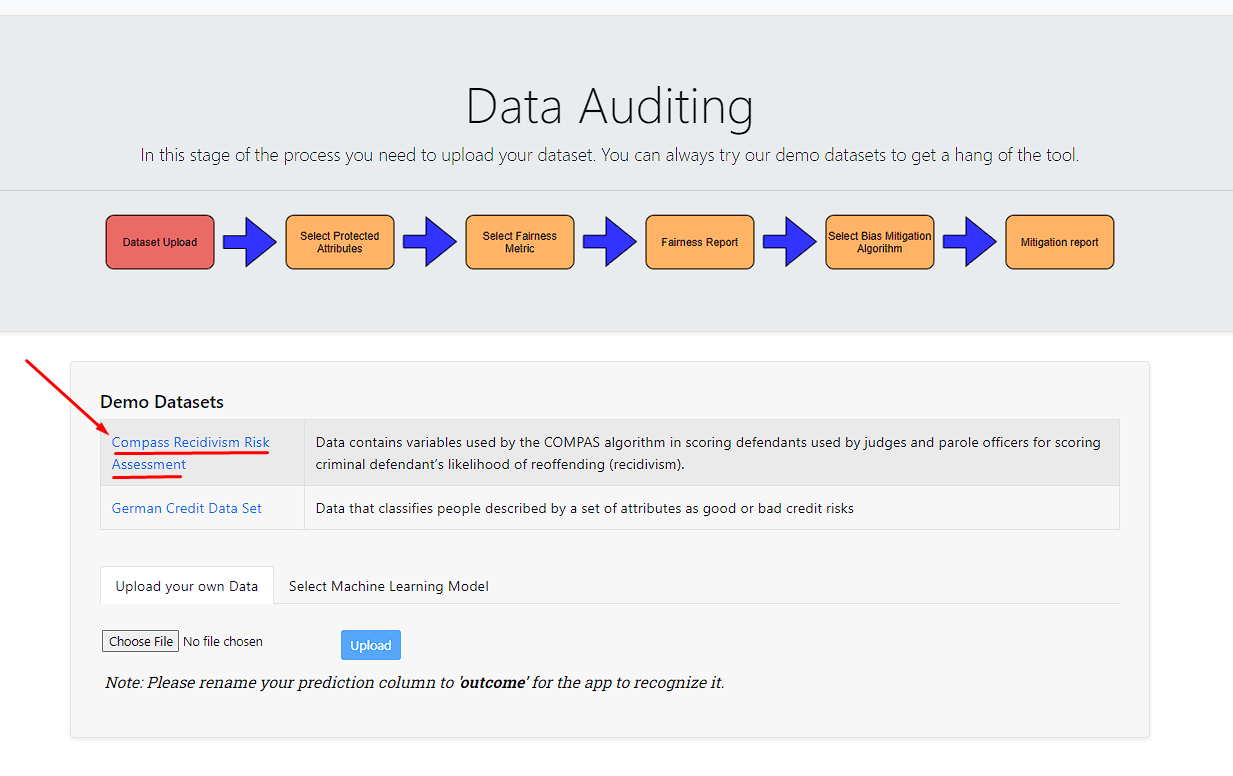
\includegraphics[width=150mm]{demo_selection_page.png}
\caption{\gr  Σελίδα επιλογής δεδομένων \label{overflow}}
\end{figure}

\subsection{Επιλογή Προστατευόμενων Χαρακτηριστικών}

Ο χρήστης επιλέγει τα προστατευόμενα χαρακτηριστικά που επιθυμεί, στο παράδειγμα υπάρχει μία και μόνη επιλογή για διευκόλυνση του χρήστη και επεξήγηση του των προνομιούχων και μη προνομιούχων ομάδων βάσει του επιλεγμένου χαρακτηριστικού.

\begin{figure}[H]
\centering
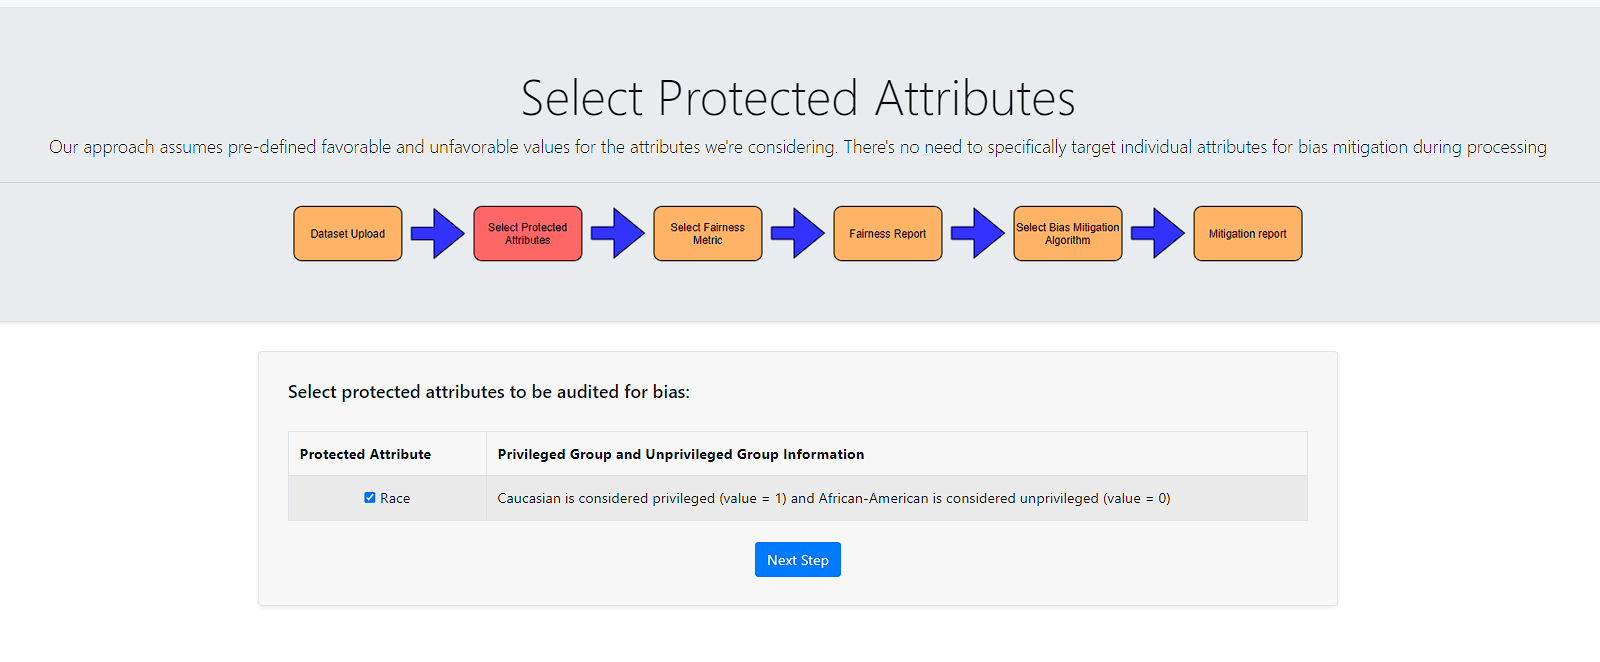
\includegraphics[width=130mm]{demo_chooseAtt.png}
\caption{\en Demo \gr Σελίδα επιλογής δεδομένων \label{overflow}}
\end{figure}


\subsection{Επιλογή Μετρικών Δικαιοσύνης}

Ο χρήστης καθοδηγείται στην επιλογή μετρικών μέσω ενός μενού που εμφανίζεται με την επιλογή "εδώ". Το μενού, σε μορφή δέντρου, οδηγεί τον χρήστη στην κατάλληλη επιλογή και αποκρύπτει τις μη σχετικές μετρήσεις.

\begin{figure}[H]
\centering
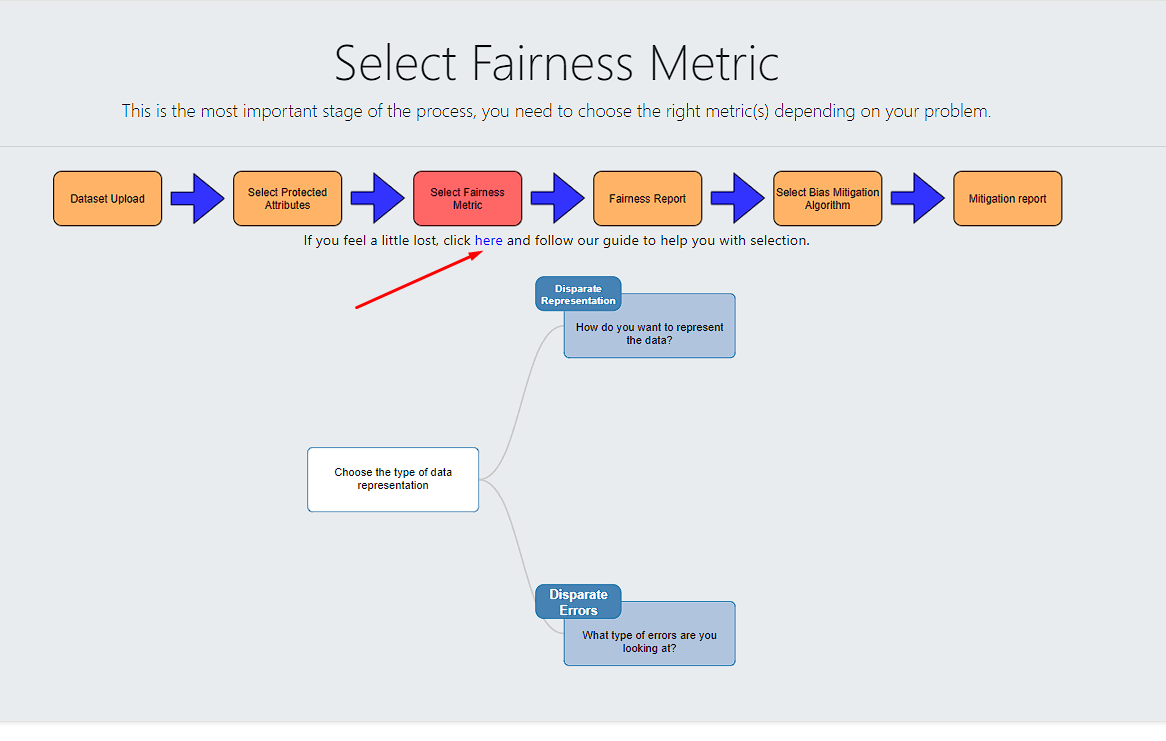
\includegraphics[width=100mm]{demo_metric_guide.png}
\caption{\en User metric guide \label{overflow}}
\end{figure}


\textit{Υποθετικό Σενάριο:} Ο χρήστης επιλέγει τις παρακάτω μετρήσεις και θέτει 80 τοις εκατό το \en threshold \gr δικαιοσύνης:

\begin{table}[h]
\centering
\begin{tabular}{|c|l|}
\hline
\textbf{\#} & \textbf{Μετρική} \\ \hline
1 & Μέση Διαφορά (\en Mean Difference) \\ \hline
2 & \en Disparate Impact \\ \hline
3 & \en Average Abs Odds Difference \\ \hline
\end{tabular}
\caption{Επιλεγμένες Μετρικές Δικαιοσύνης Εκπαιδευτικής Διαδικασίας}
\label{tab:metrics}
\end{table}

\begin{figure}[H]
\centering
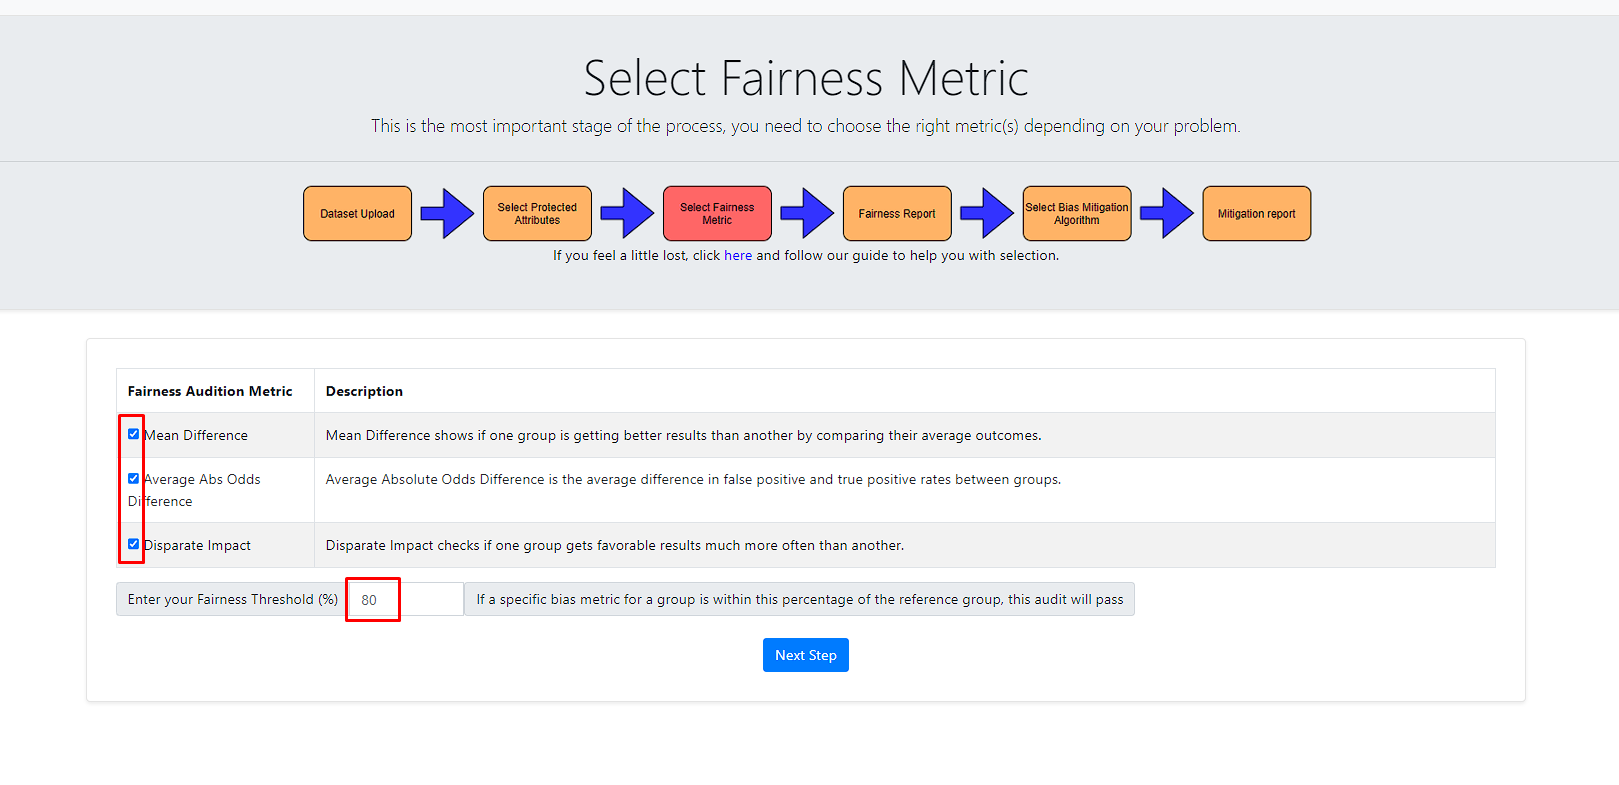
\includegraphics[width=150mm]{demo_metric_selection.png}
\caption{\en Demo \gr Επιλογή Μετρικών Δικαιοσύνης \label{overflow}}
\end{figure}

\subsection{Παρουσίαση Αποτελεσμάτων Μετρικών Δικαιοσύνης}

Εμφανίζονται οι τιμές των μετρικών και οι χαρακτηριστικές τιμές απόδοσης του συστήματος σε μορφή πινάκων και γραφημάτων.

\begin{figure}[H]
\centering
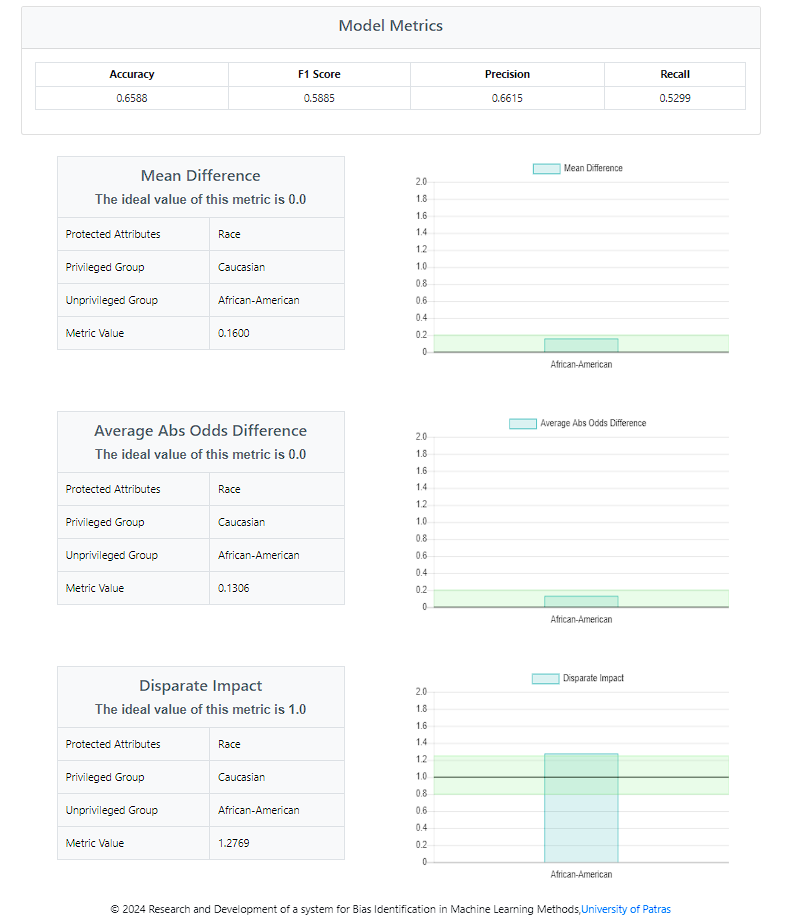
\includegraphics[width=150mm]{demo_fairness_report.png}
\caption{\en Demo \gr Επιλογή Μετρικών Δικαιοσύνης \label{overflow}}
\end{figure}

\subsection{Επιλογή Αλγορίθμων Μείωσης Μεροληψίας}

Ο χρήστης λαμβάνει ανάλυση για την επιλογή του κατάλληλου αλγορίθμου με βάσει των περιορισμών, που του έχουν τεθεί

\textit{Υποθετικό Σενάριο:} Ο χρήστης επιλέγει  αναπροσαρμογή Βαρών (\en Reweighing) \& Adversarial Debiasing \gr από τους διαθέσιμους αλγορίθμους μείωσης μεροληψίας:

\begin{figure}[H]
\centering
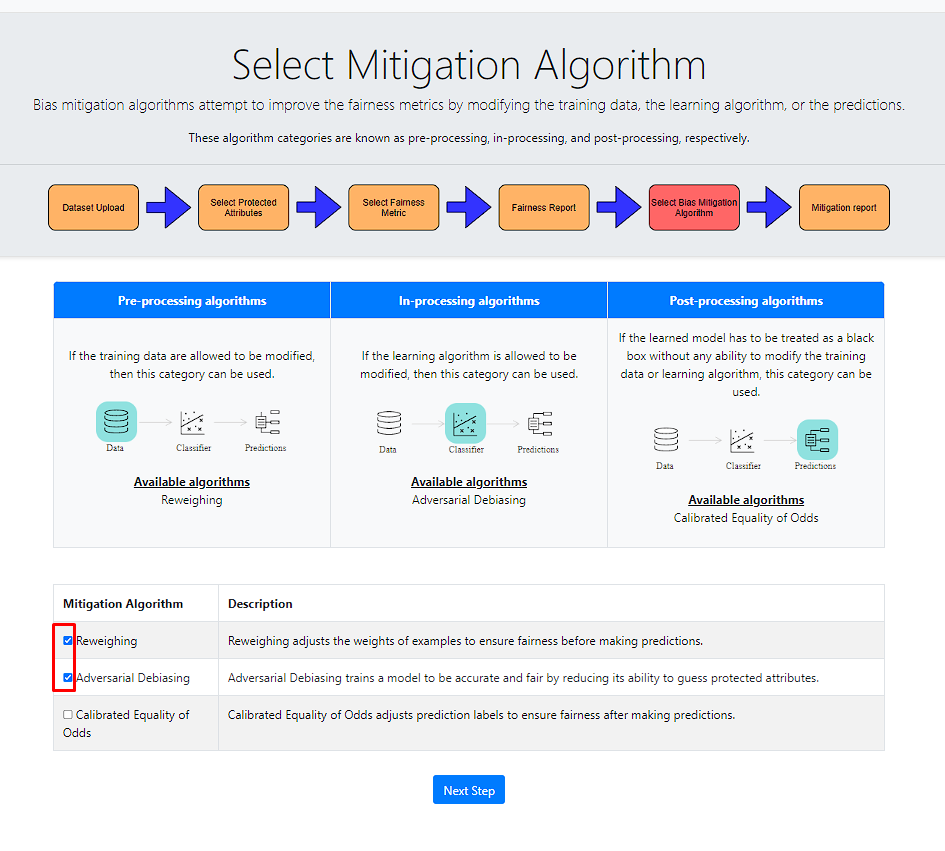
\includegraphics[width=120mm]{demo_algorithm_selection.png}
\caption{\en Demo \gr Επιλογή Αλγορίθμων Μείωσης Μεροληψίας \label{overflow}}
\end{figure}

\subsection{Τελικά Αποτελέσματα}

Εμφανίζονται οι τιμές των επιλεγμένων μετρικών μετά την εφαρμογή των αλγορίθμων.

\begin{figure}[H]
\centering
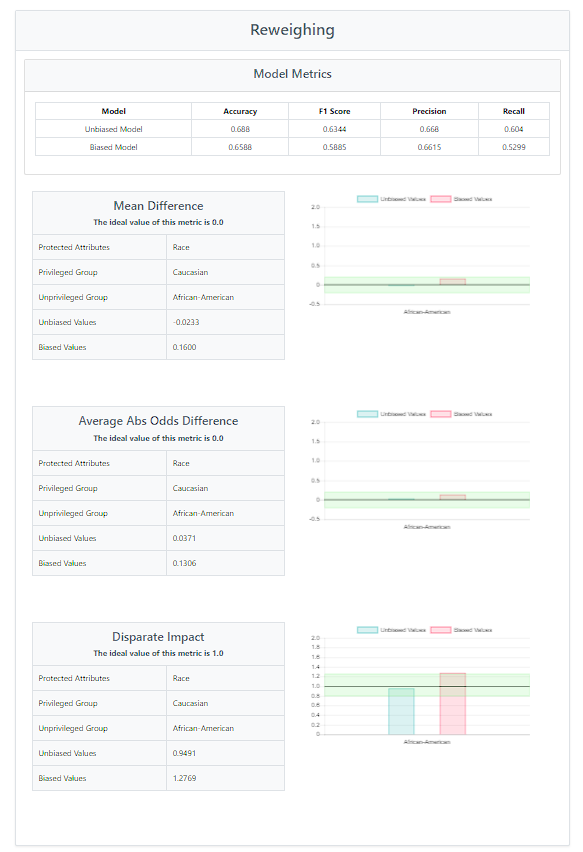
\includegraphics[width=150mm]{demo_results_1.png}
\caption{\en Demo \gr Επιλογή Αλγορίθμων Μείωσης Μεροληψίας \label{overflow}}
\end{figure}

\begin{figure}[H]
\centering
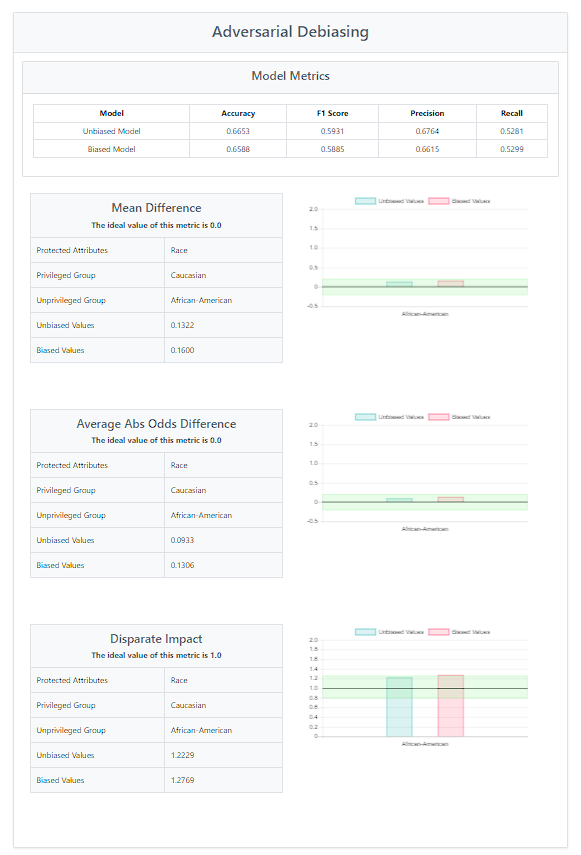
\includegraphics[width=150mm]{demo_results_2.png}
\caption{\en Demo \gr Επιλογή Αλγορίθμων Μείωσης Μεροληψίας \label{overflow}}
\end{figure}

\newpage
%%%%%%%%%%%%%%%%%%%%%%%%%%%%%%%%%%%%%%%%%%%%%%%%%%%%%%%
\section{Πειραματική Διαδικασία}

Αυτή η ενότητα περιγράφει λεπτομερώς τη διαδικασία υλοποίησης ενός πειράματος, όπου ο χρήστης αξιοποιεί το εργαλείο για να λάβει τα επιθυμητά αποτελέσματα, χρησιμοποιώντας το δικό του σύνολο δεδομένων (\en dataset)\gr.


\subsection{Επιλογή και Περιγραφή \en Dataset\gr}

Για τη μελέτη μας επιλέξαμε το \en Utrecht Fairness Recruitment Dataset \cite{utrecht_fairness_recruitment}\gr, το οποίο περιέχει τις αποφάσεις πρόσληψης τεσσάρων εταιρειών για 500 υποψηφίους. Για κάθε υποψήφιο, έχουμε διαθέσιμες κάποιες γενικές περιγραφές (\en gender, age, sport\gr) και μερικούς δείκτες. Το συγκεκριμένο \en dataset \gr είναι συνθετικό και επιλογή αυτού του  έγινε λόγω της δυνατότητας που προσφέρει για εξάσκηση στην ανάλυση ζητημάτων δικαιοσύνης.

\subsection{Επιλογή Μοντέλου Μηχανικής Μάθησης}

Η επιλογή του κατάλληλου μοντέλου μηχανικής μάθησης είναι κρίσιμη για την επιτυχία του πειράματος. Με δεδομένα τα χαρακτηριστικά του \en  dataset  \gr  και τις απαιτήσεις της ταξινόμησης, επιλέξαμε να χρησιμοποιήσουμε το μοντέλο \en{Logistic Regression}\gr.

\begin{itemize}
\item \textbf{Κατάλληλη για \en Binary Classification}:  \gr Η λογιστική παλινδρόμηση έχει σχεδιαστεί ειδικά για προβλήματα όπου η μεταβλητή \en{outcome} \gr λαμβάνει μόνο δύο τιμές , ταιριάζοντας ιδανικά με τη φύση της στήλης \en{outcome} \gr στο σύνολο δεδομένων σας \cite{das2024logistic}.
\item \textbf{Ερμηνεύσιμα Αποτελέσματα}: Παρέχει συντελεστές που μπορούν να ερμηνευθούν εύκολα. Κάθε συντελεστής αντιπροσωπεύει την επίδραση μιας μονάδας αλλαγής στη μεταβλητή πρόβλεψης στις λογαριθμικές πιθανότητες της έκβασης, προσφέροντας πολύτιμες πληροφορίες για τη σχέση μεταξύ των παραγόντων πρόβλεψης και της τελικής έκβασης.
\item \textbf{Πιθανολογικές Προβλέψεις}: Σε αντίθεση με άλλα μοντέλα ταξινόμησης που παρέχουν απλώς κατηγοριοποιημένες προβλέψεις, η λογιστική παλινδρόμηση παράγει πιθανολογικές εξόδους. Αυτό προσφέρει μια πιο λεπτομερή κατανόηση των προβλέψεων, επιτρέποντας λήψη αποφάσεων με βάση κατώφλια πιθανότητας.
\item \textbf{Ευελιξία και Ανθεκτικότητα}: Το αποτέλεσμα του μοντέλου βασίζεται σε λιγότερες υποθέσεις σε σύγκριση με εναλλακτικές μεθόδους ταξινόμησης, όπως η διακριτική ανάλυση. Χάρη σε αυτό, η λογιστική παλινδρόμηση αποδεικνύεται ανθεκτική σε ένα ευρύ φάσμα πρακτικών καταστάσεων\cite{bucker2022transparency}.
\end{itemize}

Συνοψίζοντας, η επιλογή του \en{Logistic Regression}\gr είναι βάσιμη λόγω της απλότητάς του, της ερμηνευσιμότητας των αποτελεσμάτων του, της ανθεκτικότητάς του σε υπερπροσαρμογή και της αποτελεσματικότητάς του σε προβλήματα δυαδικής ταξινόμησης, εξασφαλίζοντας υψηλή απόδοση και αξιοπιστία.

\begin{figure}[H]
\centering
\includegraphics[width=110mm]{dutch_choose_model.png}
\caption{\en Demo \gr Επιλογή  Μοντέλου Κατά τη Χρήση του Εργαλείου \label{overflow}}
\end{figure}

\subsection{Ανάλυση \en Dataset\gr}

Το \en dataset \gr περιέχει 4000 εγγραφές και 14 στήλες. Δεν υπάρχουν ελλείπουσες τιμές στο \en dataset\gr. Η μεταβλητή-στόχος (\en target variable\gr) είναι το \en outcome\gr, το οποίο είναι δυαδικό (0 ή 1).\\

\subsubsection{Κατηγορηματικά χαρακτηριστικά:}

\begin{itemize}
    \item \textbf{\en gender\gr:} 3 μοναδικές τιμές (\en female, male, others\gr).
    \item \textbf{\en nationality\gr:} 3 μοναδικές τιμές (\en Dutch, German, Belgian\gr).
    \item \textbf{\en sport\gr:} 8 μοναδικές τιμές.
    \item \textbf{\en ind-debateclub, ind-programming\_exp, ind-international\_exp, ind-entrepeneur\_exp, ind-exact\_study\gr:} Δυαδικά χαρακτηριστικά (\en True/False\gr).
    \item \textbf{\en ind-degree\gr:} 3 μοναδικές τιμές (\en bachelor, master, phd\gr).
    \item \textbf{\en company\gr:} 4 μοναδικές τιμές (\en A, B, C, D\gr).
\end{itemize}

\subsubsection{Αριθμητικά χαρακτηριστικά:}

\begin{itemize}
    \item \textbf{\en age\gr:} Συνεχής μεταβλητή με μέσο όρο 26.18 χρόνια.
    \item \textbf{\en ind-university\_grade\gr:} Συνεχής μεταβλητή με μέσο όρο 62.38.
    \item \textbf{\en ind-languages\gr:} Διακριτή μεταβλητή (0, 1, 2, 3).
\end{itemize}

\subsubsection{Σημαντικότητα Χαρακτηριστικών}

Η σημαντικότητα των χαρακτηριστικών είναι μια τεχνική που χρησιμοποιείται για να αξιολογηθεί η συνεισφορά κάθε χαρακτηριστικού στην πρόβλεψη. Η ανάλυση αυτή επιτρέπει την κατανόηση των πιο κρίσιμων χαρακτηριστικών που επηρεάζουν το αποτέλεσμα του μοντέλου.

 Το γράφημα που ακολουθεί παρουσιάζει τη σημαντικότητες των χαρακτηριστικών, ταξινομημένες κατά φθίνουσα σειρά:
\begin{figure}[H]
\centering
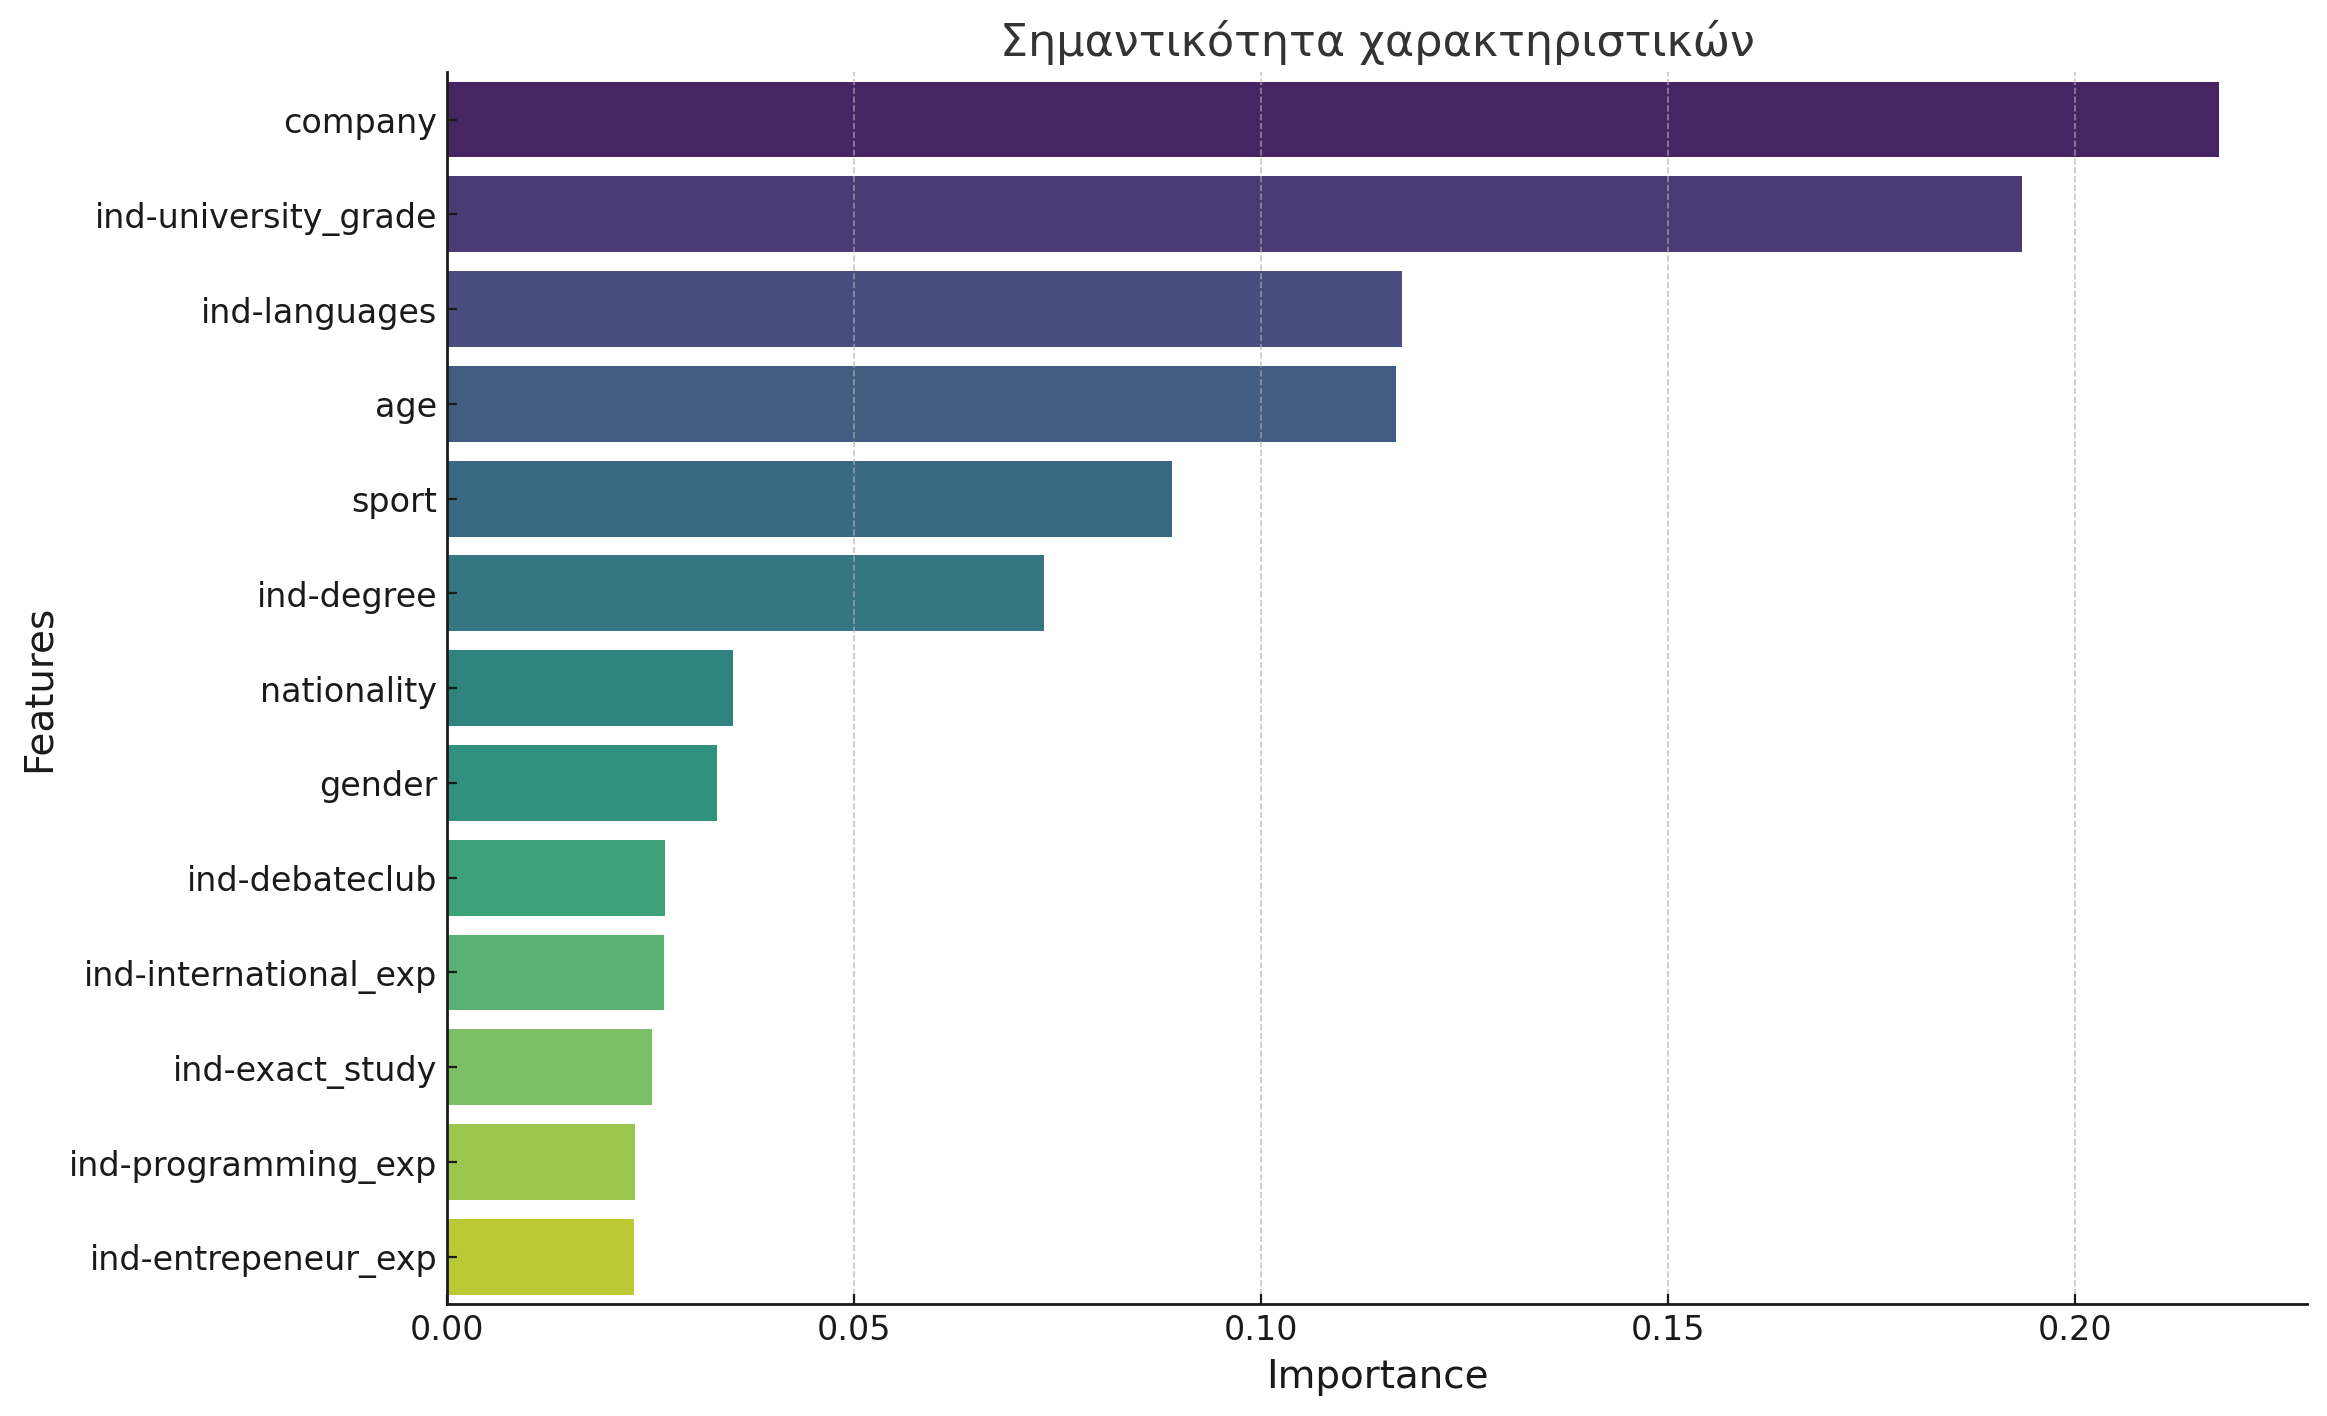
\includegraphics[width=170mm]{feature_importance.png}
    \caption{Σημαντικότητα Χαρακτηριστικών}
    \label{fig:feature_importance}
\end{figure}

\subsubsection{Συσχέτιση Χαρακτηριστικών}

 Το γράφημα που ακολουθεί παρουσιάζει τη σημαντικότητα των χαρακτηριστικών, ταξινομημένες κατά φθίνουσα σειρά:
\begin{figure}[H]
\centering
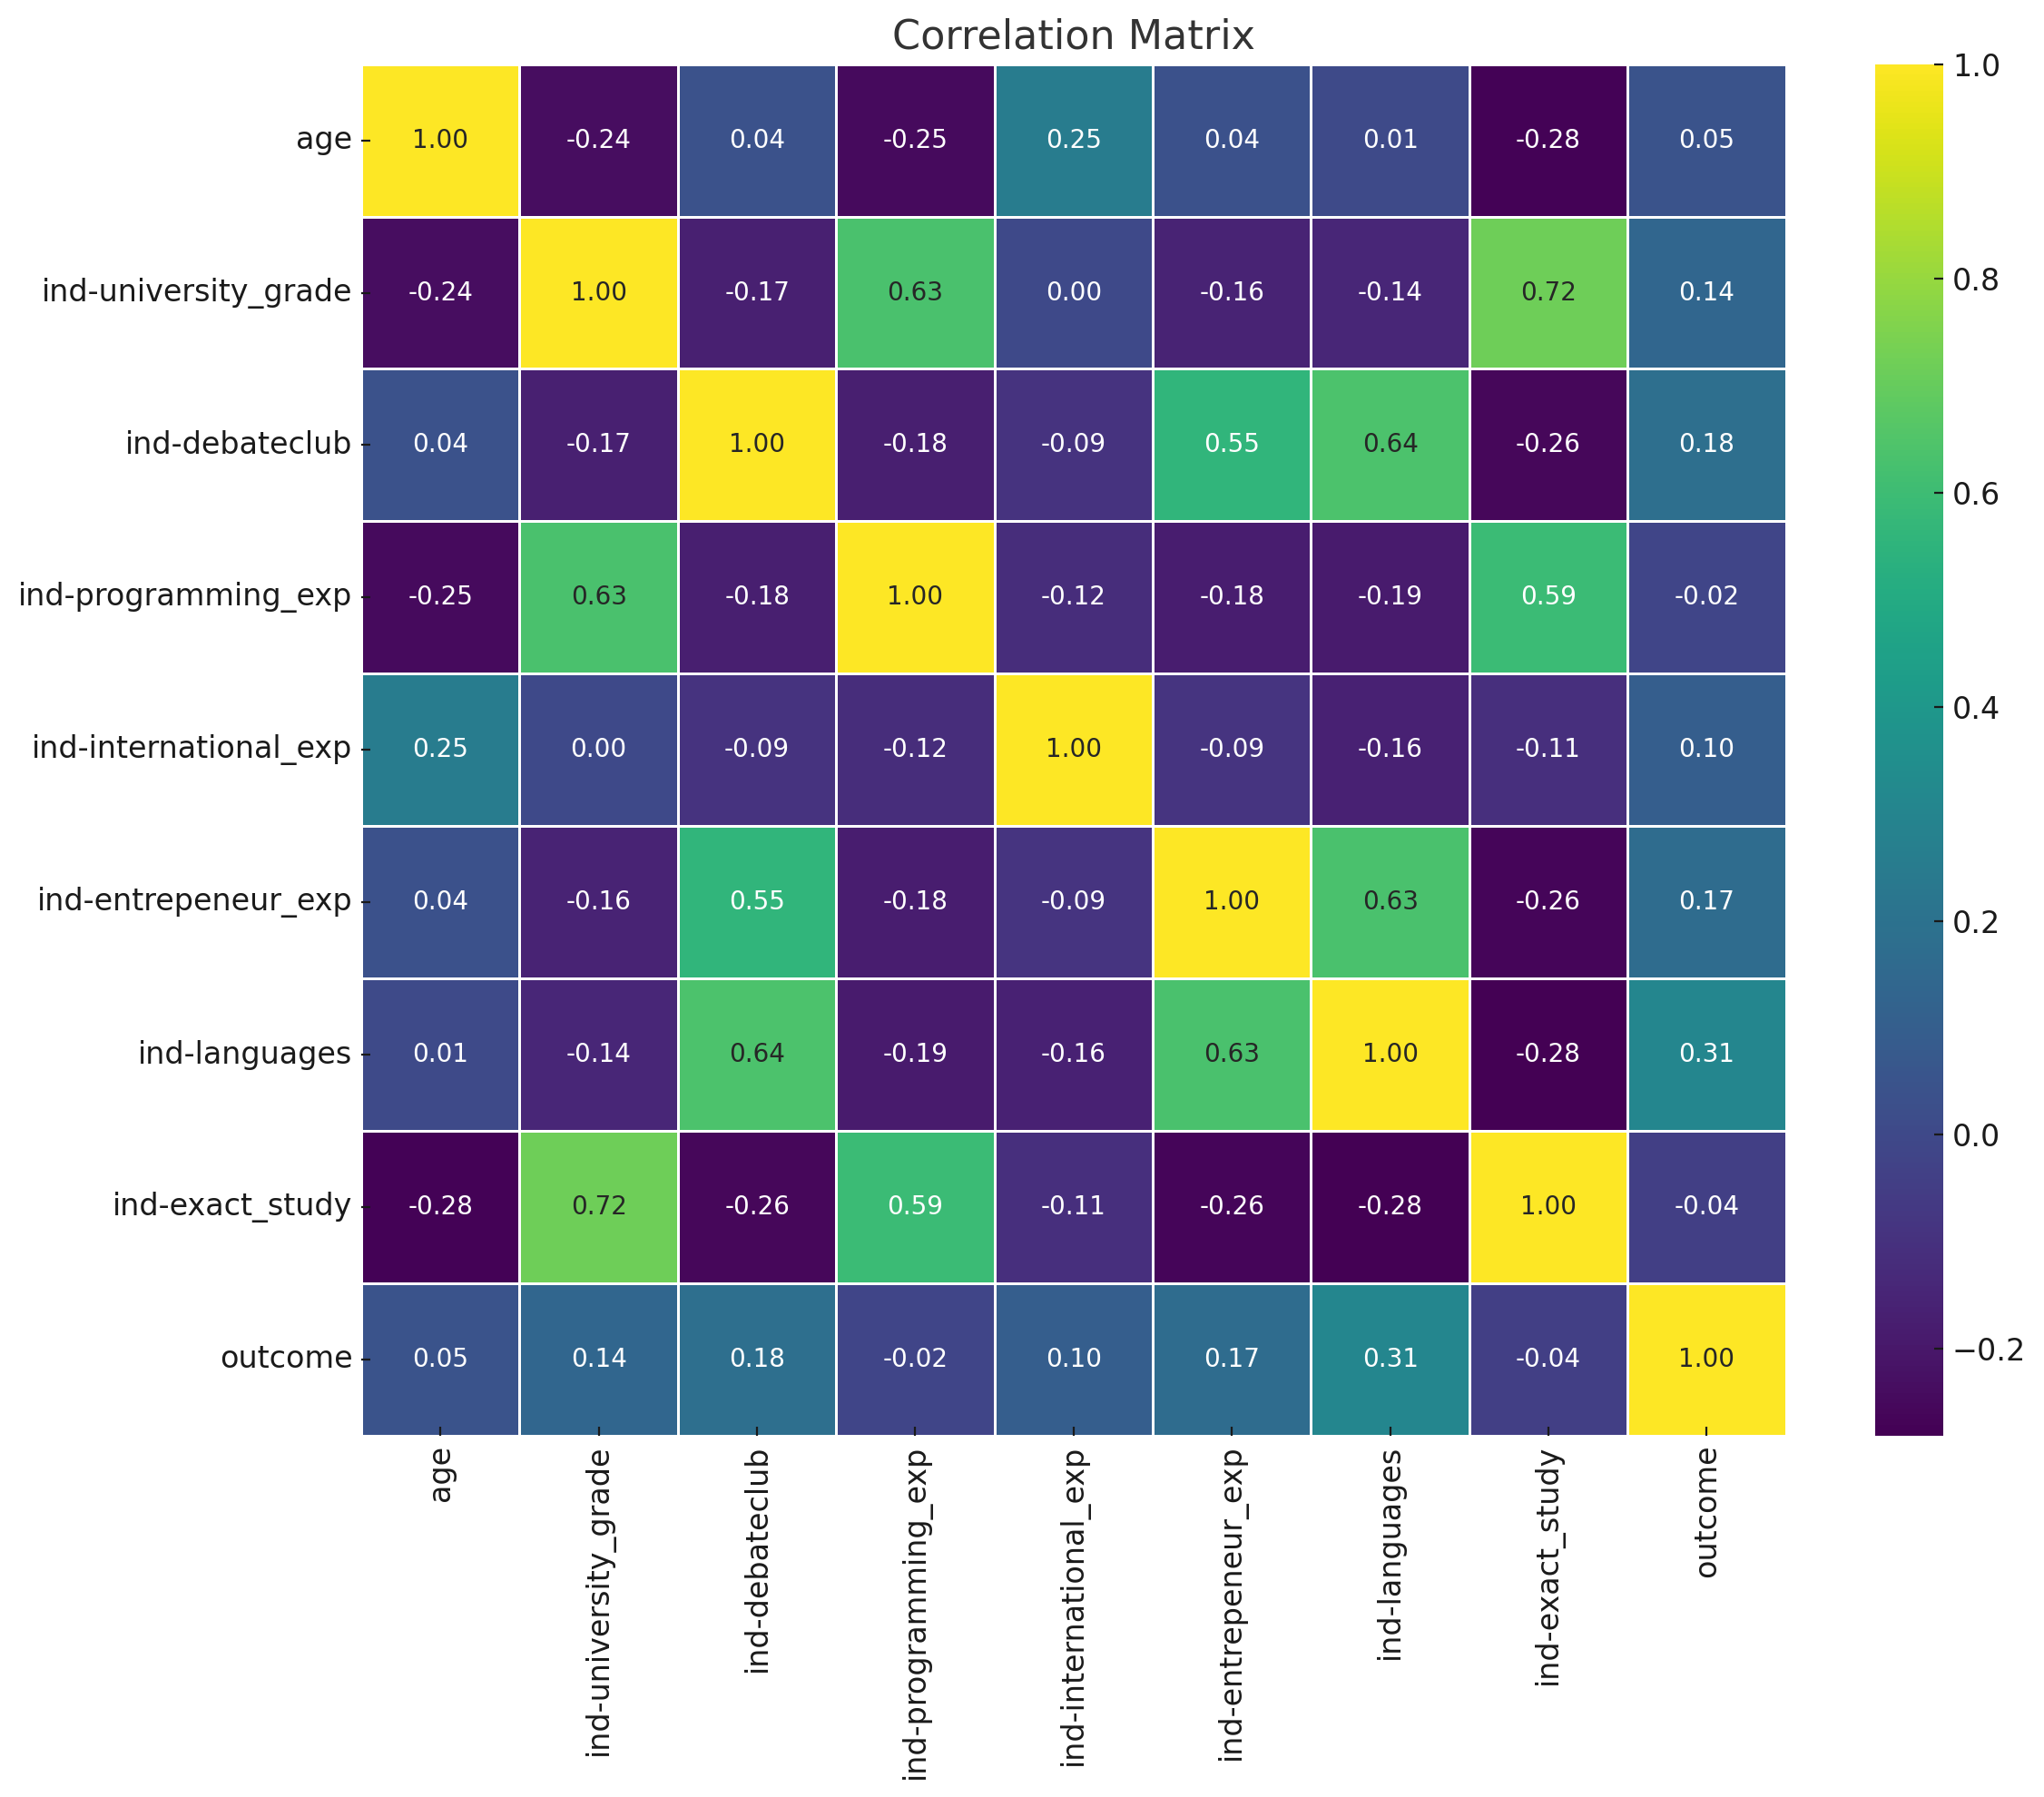
\includegraphics[width=120mm]{correlation_matrix.png}
    \caption{Συσχέτηση Χαρακτηριστικών}
    \label{fig:correlation_matrix}
\end{figure}

Βασισμένα στη συσχέτιση των χαρακτηριστικών με το αποτέλεσμα (\en{outcome}\gr), μπορούμε να εξάγουμε τα ακόλουθα συμπεράσματα: Το χαρακτηριστικό \en{ind-languages}\gr έχει την υψηλότερη θετική συσχέτιση με το αποτέλεσμα (\( r = 0.31 \)). Αυτό σημαίνει ότι ο αριθμός των γλωσσών που γνωρίζει ένας υποψήφιος επηρεάζει θετικά την πιθανότητα πρόσληψής του. Αντίθετα, το χαρακτηριστικό \en{ind-exact\_study}\gr έχει την χαμηλότερη συσχέτιση με το αποτέλεσμα (\( r = -0.04 \)). Αυτό υποδηλώνει ότι η ακριβής μελέτη του υποψηφίου δεν έχει σημαντική επίδραση στην πιθανότητα πρόσληψής του.

Γενικά, οι τιμές των συσχετίσεων δείχνουν ότι τα περισσότερα χαρακτηριστικά έχουν χαμηλή συσχέτιση με το αποτέλεσμα. Αυτό σημαίνει ότι δεν υπάρχει κάποιο χαρακτηριστικό που από μόνο του να καθορίζει την πιθανότητα πρόσληψης των υποψηφίων. Αντιθέτως, η απόφαση για την πρόσληψη φαίνεται να εξαρτάται από έναν συνδυασμό πολλών διαφορετικών χαρακτηριστικών.

\subsection{Επιλογή Προστατευμένων Χαρακτηριστικών και Ομάδων}

Για την αξιολόγηση των διασταυρούμενων χαρακτηριστικών, εξετάστηκαν διάφοροι συνδυασμοί φύλου και εθνικότητας. Τα αποτελέσματα συνοψίζονται στον παρακάτω πίνακα\en:

\begin{table}[H]
\centering
\begin{tabular}{|p{2cm}|p{3cm}|p{7cm}|p{2cm}|}
\hline
\textbf{Gender} & \textbf{Nationality} & \textbf{Actual Outcome Mean} & \textbf{Count} \\ \hline
female & Belgian  & 0.260870 & 46 \\ \hline
female & Dutch & 0.252336 & 428 \\ \hline
female & German & 0.217391 & 46 \\ \hline
male & Belgian & 0.320000 & 75 \\ \hline
male & Dutch  & 0.328740 & 508 \\ \hline
male & German  & 0.405063 & 79 \\ \hline
\end{tabular}
\caption{\gr Συνδυασμοί φύλου και εθνικότητας με μέσους όρους προβλεπόμενων και πραγματικών αποτελεσμάτων}
\label{tab:cross_features}
\end{table}

\begin{figure}[H]
\centering
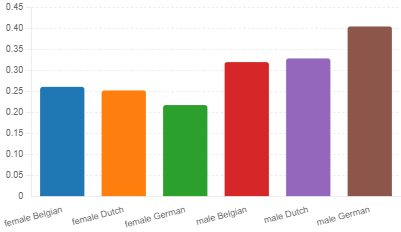
\includegraphics[width=100mm]{intersectional_mean.png}
\caption{\gr Συνδυασμοί φύλου και εθνικότητας με μέσους όρους \label{overflow}}
\end{figure}

\gr Από το σύνολο δεδομένων, θα επιλεχτούν οι συνδυασμοί φύλου και εθνικότητας, \en{male Dutch} \gr και \en{female Belgian}\gr. Μεγαλύτερα δείγματα προσφέρουν πιο στενά διαστήματα εμπιστοσύνης, μειώνοντας την αβεβαιότητα των εκτιμήσεων. Καθώς αυξάνεται το μέγεθος δείγματος, τα διαστήματα εμπιστοσύνης γίνονται στενότερα, παρέχοντας πιο ακριβείς εκτιμήσεις για παραμέτρους όπως το μέσο βάρος ή το ύψος. Αυτό οφείλεται στο ότι μεγαλύτερα δείγματα μειώνουν την τυπική απόκλιση του μέσου όρου του δείγματος, κάνοντας την εκτίμηση πιο αξιόπιστη.\cite{statology2021}

\gr Η επιλογή των χαρακτηριστικών φύλου και εθνικότητας, ατομικά και σε συνδυασμό, για την εξέταση της αλγοριθμικής δικαιοσύνης είναι κρίσιμη για διάφορους λόγους. Στατιστικά στοιχεία δείχνουν ότι γυναίκες και άνδρες βιώνουν διαφορετικές ευκαιρίες και μεταχείριση σε διάφορους τομείς, όπως η απασχόληση, η εκπαίδευση και η υγειονομική περίθαλψη. Η ενσωμάτωση του φύλου στα μοντέλα επιτρέπει τον εντοπισμό και την αντιμετώπιση προκαταλήψεων που μπορεί να οδηγήσουν σε ανισότητες στις προβλέψεις \cite{schumann2020we}. Η εθνικότητα σχετίζεται με κοινωνικοοικονομικές διαφορές, πρόσβαση σε πόρους και ευκαιρίες, και ιστορικές ανισότητες. Η ανάλυση βάσει εθνικότητας βοηθά στην αποκάλυψη προκαταλήψεων που βασίζονται σε στερεότυπα και διακρίσεις \cite{tang2023and}. Η ανάλυση αλγοριθμικής δικαιοσύνης με βάση τα παραπάνω χαρακτηριστικά εντοπίζει και αντιμετωπίζει συστημικές ανισότητες. Η διαφάνεια και η λογοδοσία είναι απαραίτητες για την προστασία των δικαιωμάτων και την ισότιμη μεταχείριση όλων των πολιτών. Η συνειδητή λήψη αποφάσεων με βάση τα δεδομένα προωθεί την κοινωνική δικαιοσύνη και την ισότητα ευκαιριών. Η επιλογή φύλου και εθνικότητας, ατομικά και σε συνδυασμό, είναι απαραίτητη για την ανάπτυξη δίκαιων και αξιόπιστων αλγορίθμων.

\begin{figure}[H]
\centering
\includegraphics[width=120mm]{dutch_choose_att.png}
\caption{\gr Επιλογή Προστατευμένων Χαρακτηριστικών και Ομάδων \label{overflow}}
\end{figure}


\subsection{Επιλογή Μετρικών Δικαιοσύνης}

Θα αξιοποιήσουμε τη μετρική \en{disparate impact} \gr σε συνδυασμό με αναλύσεις συνδυασμών φύλου και εθνικότητας. Στόχος μας είναι να διασφαλίσουμε ότι το μοντέλο μας λαμβάνει υπόψη τις αλληλεπιδράσεις μεταξύ αυτών των χαρακτηριστικών και να αποφεύγουμε τυχόν δυσανάλογη επίδραση σε συγκεκριμένες υποομάδες. Η μετρική \en{disparate impact} \gr αποτελεί μια ευρέως αναγνωρισμένη μετρική για τον εντοπισμό διακρίσεων σε αλγοριθμικές αποφάσεις. Εστιάζει στην σύγκριση των αποτελεσμάτων μεταξύ διαφορετικών ομάδων, επισημαίνοντας τυχόν δυσανάλογη επίδραση σε προστατευόμενες ομάδες\cite{kassir2023ai}.

 Η χρήση της επιτρέπει την αξιολόγηση της αλγοριθμικής δικαιοσύνης σε ένα πιο πρακτικό και νομικά αποδεκτό πλαίσιο. Σε πλήθος νομοθεσιών, η έννοια του \en{disparate impact} \gr έχει ήδη ενσωματωθεί, καθιστώντας τη μετρική αυτή απαραίτητη για την τήρηση των νομοθετικών προδιαγραφών \cite{barocas2016big}.

Τέλος, ευθυγραμμίζεται με τους στόχους μας για την προώθηση της ισότητας και της κοινωνικής δικαιοσύνης, παρέχοντας ένα αξιόπιστο εργαλείο για την συνεχή παρακολούθηση και βελτίωση της δικαιοσύνης των αλγορίθμων μας.

\begin{figure}[H]
\centering
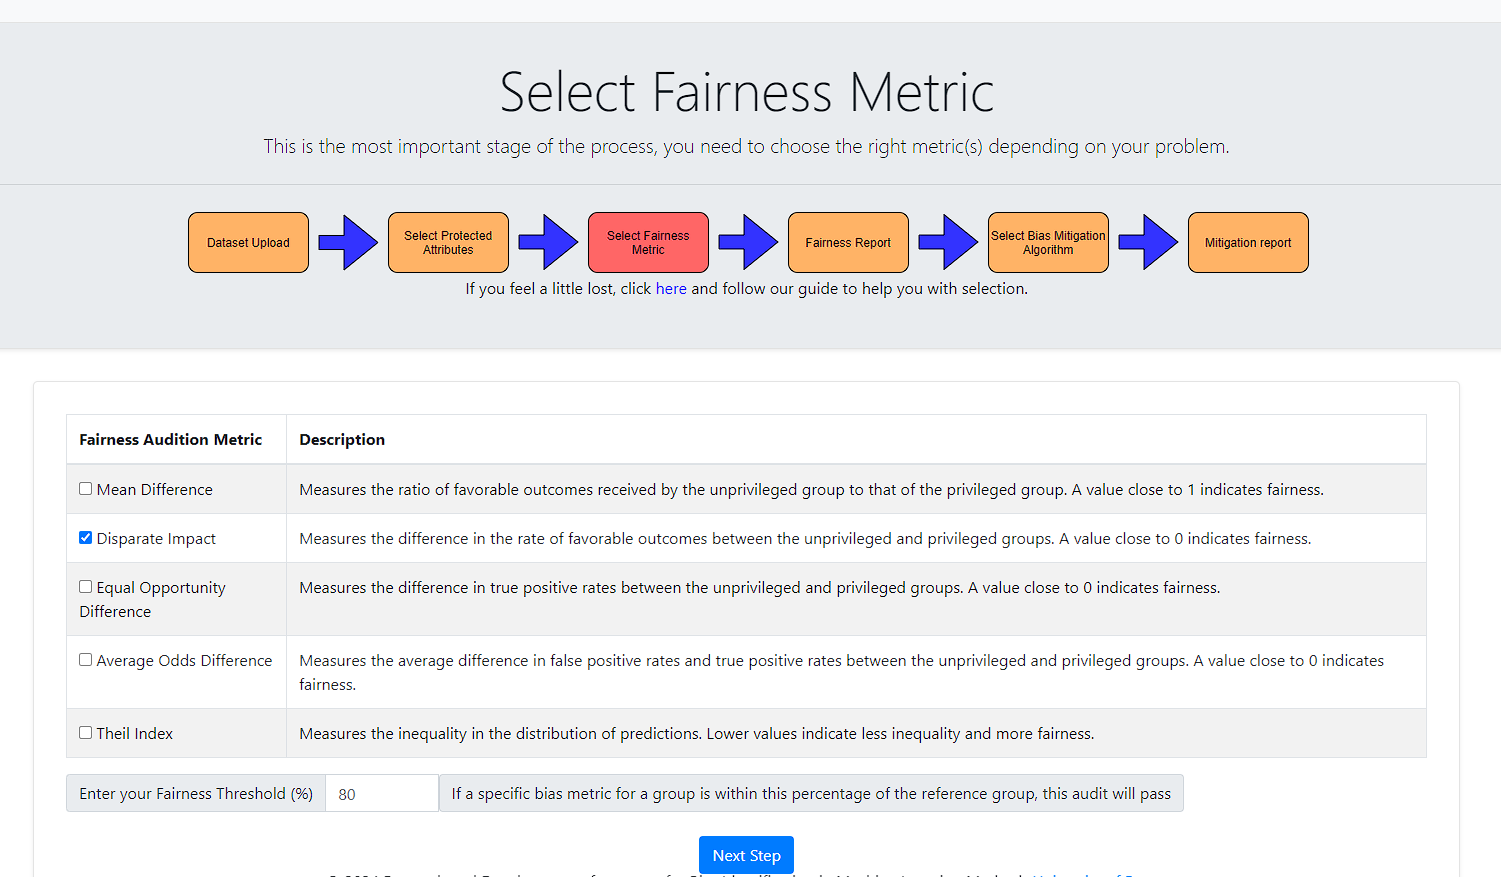
\includegraphics[width=120mm]{dutch_metric_selection.png}
\caption{\gr Επιλογή Μετρικών Δικαιοσύνης \label{overflow}}
\end{figure}


\subsection{Επιλογή Αλγορίθμου Μείωσης Μεροληψίας}

Επιλέξαμε τον αλγόριθμο αναπροσαρμογής βαρών \en{Reweighing}\gr, ο οποίος αποτελεί μέθοδο που εφαρμόζεται πριν την επεξεργασία (\en{pre-processing}) \gr .Είναι ιδανικός για σενάρια όπου δεν υπάρχει πρόσβαση ή δικαίωμα επέμβασης στα αποτελέσματα ή το μοντέλο, καθώς μπορεί να εφαρμοστεί απευθείας στα δεδομένα του ταξινομητή. Αυτό είναι ιδιαίτερα σημαντικό όταν το μοντέλο θεωρείται \en «black-box» \gr και η τροποποίηση των εσωτερικών του παραμέτρων δεν είναι δυνατή.

\begin{enumerate}
    \item \textbf{Αποτελεσματικότητα}: Η Αναπροσαρμογή Βαρών έχει αποδειχθεί ιδιαίτερα αποτελεσματική στη μείωση της μεροληψίας σε διάφορα σενάρια. Αυτό συμβαίνει επειδή η μέθοδος λαμβάνει υπόψη τα στατιστικά χαρακτηριστικά των δεδομένων εκπαίδευσης, προσαρμόζοντας τα βάρη δειγμάτων με στόχο την εξισορρόπηση των πιθανοτήτων σφάλματος μεταξύ των ομάδων.\cite{ambel2021reducing}
    \item \textbf{Ευελιξία}: Είναι μια ευέλικτη μέθοδος που μπορεί να εφαρμοστεί σε ποικίλες περιπτώσεις. Μπορεί να χρησιμοποιηθεί με γραμμικά και μη γραμμικά μοντέλα ταξινόμησης, καθώς και με δεδομένα συνεχούς και διακριτού τύπου.
    \item \textbf{Απλότητα και Ερμηνευσιμότητα}: Η Αναπροσαρμογή Βαρών είναι μια σχετικά απλή μέθοδος με εύκολη υλοποίηση και ερμηνεία.
    \item \textbf{Υπολογιστική Αποτελεσματικότητα}: Η Αναπροσαρμογή Βαρών είναι μια υπολογιστικά αποδοτική μέθοδος που μπορεί να υλοποιηθεί με σχετικά μικρό κόστος.
\end{enumerate}

Συνολικά, η Αναπροσαρμογή Βαρών αποτελεί μια ισχυρή, ευέλικτη και αποτελεσματική μέθοδο μείωσης μεροληψίας που ταιριάζει ιδανικά στις ανάγκες του έργου μας.

\begin{figure}[H]
\centering
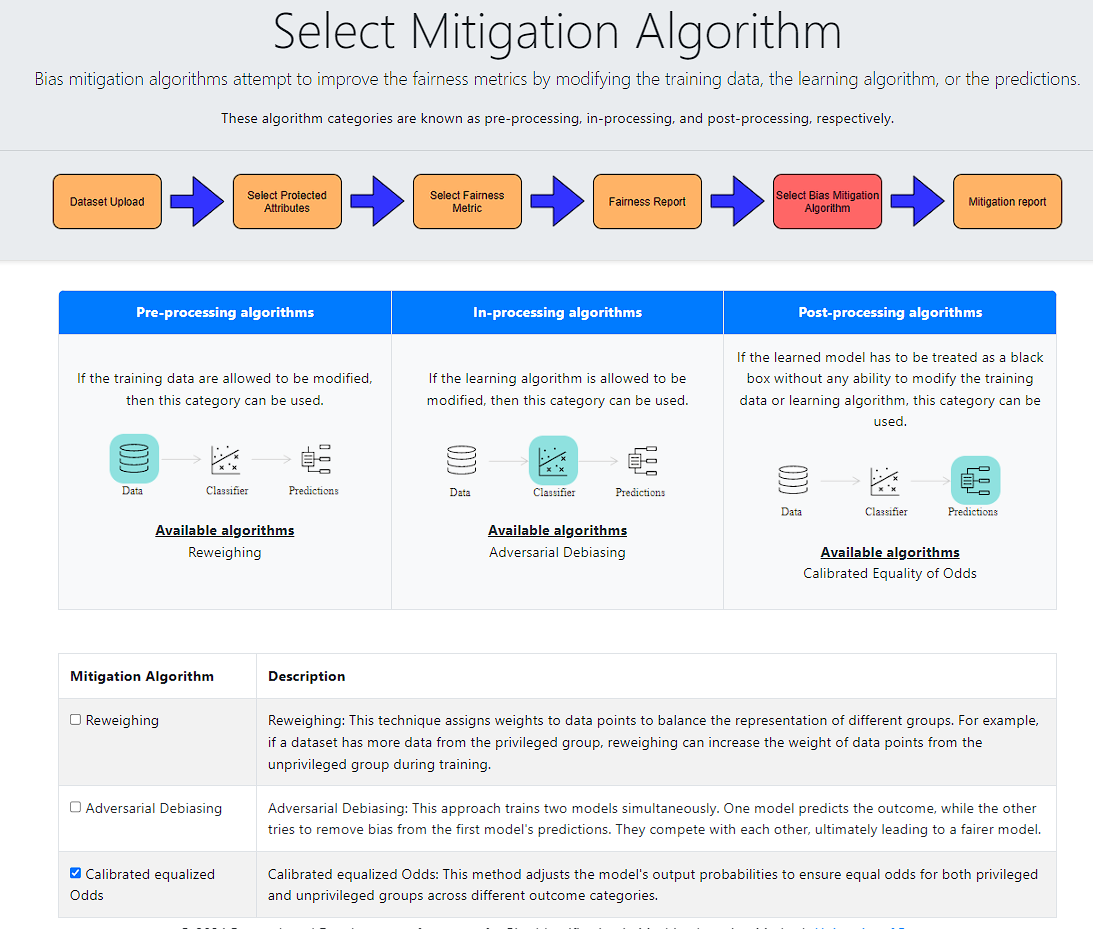
\includegraphics[width=120mm]{dutch_algorithm_selection.png}
\caption{\gr Επιλογή Αλγορίθμου Μείωσης Μεροληψίας\label{overflow}}
\end{figure}

\subsection{Αποτελέσματα Μετρικών Δικαιοσύνης}

\begin{figure}[H]
\centering
\includegraphics[width=120mm]{dutch_fairness_report.png}
\caption{\gr Αποτελέσματα Μετρικών Διακοσύνης\label{overflow}}
\end{figure}

\gr Η ανάλυση των μετρήσεων δικαιοσύνης αποκαλύπτει σημαντική μεροληψία εις βάρος των γυναικών Ολλανδικής καταγωγής. Η τιμή της μετρικής \en{ Disparate Impact } \gr  0.5539  δηλώνει οτι η πιθανότητα λήψης ευνοϊκής απόφασης για γυναίκες είναι περίπου 45\% χαμηλότερη σε σχέση με τους άνδρες. Αυτό παραβιάζει πιθανότατα το \en{Four-Fifths Rule (κανόνας 80\%)} \gr, σύμφωνα με το οποίο η αναλογία επιτυχίας μίας προστατευόμενης ομάδας δεν πρέπει να είναι μικρότερη από 80\% της αναλογίας επιτυχίας της μη προστατευόμενης ομάδας.

\textbf{Ερμηνεία}: Η πιθανότητα μίας γυναίκας Ολλανδικής καταγωγής να λάβει ευνοϊκή απόφαση είναι 55.39\%, 44.61\% χαμηλότερη από έναν άνδρα Ολλανδικής καταγωγής.Η αναλογία επιτυχίας γυναικών (0.5539) είναι κάτω από 80\% της αναλογίας επιτυχίας ανδρών γεγονός που έρχεται σε αντίθεση με τον κανόνα τεσσάρων πέμπτων.

\begin{itemize}
    \item \textbf{\en{Accuracy} \gr (Ακρίβεια Πρόβλεψης)}: Η ακρίβεια πρόβλεψης του μοντέλου είναι 0.75. Αυτό σημαίνει ότι το μοντέλο ταξινομεί σωστά το 75\% των περιπτώσεων στο σύνολο δεδομένων. Η ακρίβεια είναι μια γενική μέτρηση της απόδοσης, αλλά δεν λαμβάνει υπόψη την ισορροπία των κατηγοριών.
    
    \item \textbf{\en{F1 Score}}: \gr Η τιμή του \en{F1 Score} \gr είναι 0.4924. Η μετρική αυτή είναι ο αρμονικός μέσος όρος της ακρίβειας (\en{precision}\gr) και της ανάκλησης (\en{recall}\gr), και είναι πιο ενδεικτική της απόδοσης του μοντέλου σε περιπτώσεις με ανισορροπία κατηγοριών. Το σχετικά χαμηλό \en{F1 Score} \gr υποδεικνύει ότι το μοντέλο δυσκολεύεται να διαχειριστεί τις λανθασμένες ταξινομήσεις.
    
    \item \textbf{\en{Precision } \gr(Ακρίβεια)}: Η ακρίβεια του μοντέλου είναι 0.6025. Αυτό σημαίνει ότι από όλες τις περιπτώσεις που το μοντέλο ταξινομεί ως θετικές, το 60.25\% είναι πραγματικά θετικές. Η υψηλή ακρίβεια σημαίνει ότι το μοντέλο έχει λιγότερα ψευδώς θετικά.
    
    \item \textbf{\en{Recall } \gr (Ανάκληση)}: Η ανάκληση του μοντέλου είναι 0.4163. Αυτό σημαίνει ότι από όλες τις πραγματικά θετικές περιπτώσεις, το μοντέλο ανιχνεύει το 41.63\%. Η χαμηλή ανάκληση υποδηλώνει ότι το μοντέλο δεν ανιχνεύει όλες τις θετικές περιπτώσεις, έχοντας αρκετά ψευδώς αρνητικά.
\end{itemize}

\subsection{Αποτελέσματα Μείωσης Μεροληψίας}

\begin{figure}[H]
\centering
\includegraphics[width=120mm]{dutch_mitigation_repost.png}
\caption{\gr Αποτελέσματα  Μείωσης Μεροληψίας \label{overflow}}
\end{figure}

Με την εφαρμογή του αλγόριθμου \en{Reweighing}\gr, παρατηρούμε σημαντική βελτίωση στις μετρικές δικαιοσύνης και απόδοσης του μοντέλου. Συγκεκριμένα, η τιμή της μετρικής \en{disparate impact}\gr για τις ομάδες \en{male Dutch}\gr και \en{female Dutch}\gr είναι 0.8244. Συγκριτικά με την προηγούμενη τιμή του 0.5539, παρατηρούμε σημαντική μείωση της μεροληψίας εις βάρος των γυναικών. Το αποτέλεσμα της μείωσης είναι ικανοποιητικό και ικανοποιεί τον κανόνα των τεσσάρων πέμπτων με τα διασταυρούμενα χαρακτηριστικά φύλου και εθνικότητας.

\newpage
\begin{table}[h]
\centering
\begin{tabular}{|p{2cm}|p{6cm}|p{6cm}|}
\hline
\textbf{Μετρική} & \textbf{Πριν την εφαρμογή του αλγόριθμου  \en{Reweighing}\gr} & \textbf{Μετά την εφαρμογή του αλγόριθμου \en{Reweighing}\gr} \\
\hline
\en{Disparate Impact}\gr & 0.5539 & 0.8244 \\ \hline
\en{Accuracy}\gr & 0.75 & 0.76 \\ \hline
\en{F1 Score}\gr & 0.4924 & 0.5152 \\ \hline
\en{Precision}\gr & 0.6025 & 0.6892 \\ \hline
\en{Recall}\gr & 0.4163 & 0.4113 \\ \hline
\end{tabular}
\caption{Πίνακας με Προηγούμενες \en{Biased}\gr και \en{Unbiased}\gr Τιμές Μοντέλου}
\end{table}

\begin{itemize}
    \item \textbf{Δείκτης \en{Disparate Impact}\gr}: Η μεροληψία εις βάρος των γυναικών Ολλανδών μειώθηκε σημαντικά, από 0.5539 σε 0.8244. Αυτό σηματοδοτεί μια αισθητή βελτίωση προς την κατεύθυνση της εξάλειψης της μεροληψίας και την τήρηση της αρχής της ίσης μεταχείρισης.
    \item \textbf{Τήρηση του Κανόνα των Τεσσάρων Πέμπτων}: Η μείωση της μεροληψίας επιτυγχάνει τον κανόνα των τεσσάρων πέμπτων, ο οποίος ορίζει ότι η μεροληπτική επίδραση σε μια προστατευόμενη ομάδα δεν πρέπει να υπερβαίνει το 80\% της αντίστοιχης επίδρασης στην ομάδα αναφοράς. Στην περίπτωσή μας, η μεροληπτική επίδραση για τις γυναίκες Ολλανδές είναι τώρα 82.44\%, άρα οριακά κάτω από το όριο του 80\%.
 \item \textbf{Ακρίβεια (\en{Accuracy}\gr)}: Η ακρίβεια πρόβλεψης του μοντέλου αυξήθηκε από 0.75 σε 0.76. Αυτό υποδηλώνει ότι το μοντέλο λαμβάνει πιο σωστές προβλέψεις συνολικά.
    \item \textbf{\en{F1 Score}\gr}: Το \en{F1 Score}\gr, ένα μέτρο που συνδυάζει ακρίβεια και ανάκληση, επίσης βελτιώθηκε από 0.4924 σε 0.5152.
    \item \textbf{Ακρίβεια (\en{Precision}\gr)}: Η ακρίβεια αυξήθηκε από 0.6025 σε 0.6892.
    \item \textbf{Ανάκληση (\en{Recall}\gr)}: Η ανάκληση παρέμεινε σχεδόν σταθερή, μειώθηκε ελαφρώς από 0.4163 σε 0.4113.
\end{itemize}

\gr Σε σύγκριση με τις αρχικές μετρήσεις απόδοσης, παρατηρείται αισθητή βελτίωση μετά την υλοποίηση της μεθόδου \en{Reweighing}\gr. Αυτό υποδηλώνει καλύτερη συνολική απόδοση του μοντέλου. Ταυτόχρονα, ικανοποιείται ο περιορισμός των τεσσάρων πέμπτων με επιλεγμένα διασταυρούμενα χαρακτηριστικά, ώστε να επιτυγχάνεται και η συμμόρφωση με τον Nόμο για τον Έλεγχο Προκαταλήψεων της Νέας Υόρκης.
Είναι σημαντικό να τονιστεί ότι η μείωση της μεροληψίας δεν έρχεται πάντα σε βάρος της απόδοσης. Στην περίπτωσή μας, η εφαρμογή του \en{Reweighing} \gr απέδειξε ότι είναι εφικτό να επιτευχθούν και οι δύο στόχοι ταυτόχρονα. Η επιλογή των κατάλληλων μετρήσεων και η λεπτομερής ανάλυση των αποτελεσμάτων είναι απαραίτητες για την αξιολόγηση της αποτελεσματικότητας των τεχνικών μείωσης μεροληψίας. Η συνεχής παρακολούθηση και η αξιολόγηση του μοντέλου σε πραγματικές συνθήκες λειτουργίας είναι απαραίτητες για την διασφάλιση της μακροχρόνιας δικαιοσύνης και αμεροληψίας του.

%%%%%%%%%%%%%%%%%%%%%%%%%%%%%%%%%%%%%%%%%%%%%%%%%%%%%%%

\newpage
\section{Συμπεράσματα και Μελλοντικές Επεκτάσεις}

\subsection{Συμπεράσματα}

Η παρούσα διπλωματική εργασία εστιάζει στην ανάπτυξη ενός εργαλείου που ενισχύει την υιοθέτηση ηθικών πρακτικών στη μηχανική μάθηση, με έμφαση στην δικαιοσύνη και την αντικατοπτριστική εκπροσώπηση της κοινωνίας στα μοντέλα. Μέσα από τα πειράματα και τα αποτελέσματα που παρουσιάστηκαν, αποδεικνύεται η αποτελεσματικότητα του εργαλείου σε διάφορες πτυχές:

\begin{enumerate}
    \item \textbf{Προσβασιμότητα και Χρηστικότητα}:
	Το εργαλείο έχει σχεδιαστεί με στόχο να είναι εύχρηστο και προσβάσιμο σε χρήστες με ποικίλο επίπεδο εμπειρίας, ακόμα και σε εκείνους με περιορισμένες γνώσεις στη μηχανική μάθηση ή την έννοια της δικαιοσύνης στα δεδομένα. Για να επιτευχθεί αυτό, περιλαμβάνει αναλυτικές οδηγίες για κάθε βήμα της διαδικασίας, από την επιλογή των προστατευόμενων χαρακτηριστικών έως την ανάλυση των μετρικών, οι οποίες συνοδεύονται από λεπτομερείς εξηγήσεις. Η διεπαφή χρήστη \en (UI) \gr διαθέτει βοηθητικά μενού για την επιλογή μετρικών δικαιοσύνης, διευκολύνοντας την κατανόηση και την υλοποίηση της διαδικασίας. Επιπλέον, κάθε μετρική δικαιοσύνης συνοδεύεται από λεπτομερή επεξήγηση του σκοπού και του τρόπου υπολογισμού της, βοηθώντας τους χρήστες να ερμηνεύσουν σωστά τα αποτελέσματα. Τα αποτελέσματα παρουσιάζονται με απλές και κατανοητές σχηματικές απεικονίσεις, επιτρέποντας στους χρήστες να οπτικοποιήσουν εύκολα τα δεδομένα και να εντοπίσουν τυχόν προβλήματα μεροληψίας. Σημειώνεται ότι, ενώ το εργαλείο έχει σχεδιαστεί με γνώμονα την ευχρηστία, η αξιολόγησή του από πραγματικούς χρήστες με ποικίλο υπόβαθρο και επίπεδο εμπειρίας είναι απαραίτητη για να επιβεβαιωθεί η αποτελεσματικότητά του.
    
    \item \textbf{Συνολική Αξιολόγηση της Δικαιοσύνης}:
    
    Το εργαλείο επιτρέπει τον έλεγχο της δικαιοσύνης σε όλα τα στάδια της ανάπτυξης ενός μοντέλου:
    \begin{itemize}
        \item \textbf{Δεδομένα}: Αξιολόγηση τυχόν μεροληψίας στα δεδομένα εκπαίδευσης.
        \item \textbf{Μοντέλο}: Ανάλυση του ίδιου του μοντέλου για τυχόν μεροληπτικές συμπεριφορές.
        \item \textbf{Αποτελέσματα}: Έλεγχος για δίκαιη και ισότιμη αντιμετώπιση όλων των ομάδων.
    \end{itemize}
    Η ευελιξία του εργαλείου επιτρέπει στον χρήστη να εστιάσει στους τομείς που έχει δικαίωμα να επέμβει, λαμβάνοντας υπόψη τυχόν περιορισμούς.
    
    \item \textbf{Εφαρμογή σε Πραγματικά Σενάρια}:
    
    Το εργαλείο έχει σχεδιαστεί για να λειτουργεί σε πραγματικές συνθήκες, λαμβάνοντας υπόψη νομικούς κανονισμούς και ηθικές πρακτικές. Συγκεκριμένα, η συμμόρφωση με τον  Νόμο  για τον Έλεγχο Προκαταλήψεων της Νέας Υόρκης  αποτελεί εγγύηση για την ηθική και νόμιμη χρήση του \cite{hilliard2022regulating}.
    
    \item \textbf{Αναγνώριση της Πολυπλοκότητας της Ανθρώπινης Ταυτότητας}:
    
    Η προσέγγιση που υιοθετεί το εργαλείο λαμβάνει υπόψη την πολυπλοκότητα της ανθρώπινης ταυτότητας. Αναγνωρίζει ότι οι άνθρωποι ανήκουν σε πολλές ομάδες ταυτόχρονα (π.χ. φύλο, φυλή, κοινωνικοοικονομική τάξη) και η δίκαιη αντιμετώπιση οφείλει να λαμβάνει υπόψη τις αλληλεπιδράσεις μεταξύ αυτών των ομάδων.

\item \textbf{Ελευθερία και Ανοιχτός Κώδικας}:
	Το εργαλείο που αναπτύξαμε είναι ανοιχτού κώδικα \en (open source), \gr κάτι που σημαίνει ότι μπορεί να χρησιμοποιηθεί από οποιονδήποτε, από φοιτητές μέχρι επαγγελματίες. Αυτή η ανοιχτότητα έχει πολλαπλά πλεονεκτήματα. Διευκολύνει τη συνεργασία και την ανταλλαγή γνώσεων, καθώς οι χρήστες μπορούν να συμβάλλουν στη βελτίωση και την επέκταση του εργαλείου. Προωθεί τη διαφάνεια, επιτρέποντας σε όλους να δουν και να κατανοήσουν πώς λειτουργεί το εργαλείο, γεγονός που ενισχύει την εμπιστοσύνη στη χρήση του. Τέλος, προσφέρει τη δυνατότητα προσαρμογής του εργαλείου στις ιδιαίτερες ανάγκες κάθε χρήστη ή οργανισμού, χωρίς περιορισμούς που μπορεί να επιβάλλουν τα εμπορικά λογισμικά. Τέλος, υποστηρίζει τη συνεχή μάθηση και την καινοτομία, καθώς παρέχει στους χρήστες την ευκαιρία να πειραματιστούν και να εφαρμόσουν νέες ιδέες στη μηχανική μάθηση και τη δικαιοσύνη.\cite{kelty2020two,langenkamp2022open}
\end{enumerate}

\subsection{Μελλοντικές Επεκτάσεις}
Για μελλοντική έρευνα, προτείνονται οι ακόλουθες κατευθύνσεις:

\begin{enumerate}
    \item \textbf{Συμπλήρωση Περισσότερων Αλγορίθμων και Μετρικών Δικαιοσύνης}:
    
    Η ενσωμάτωση επιπρόσθετων αλγορίθμων και μετρικών δικαιοσύνης θα ενισχύσει την ικανότητα του εργαλείου να ανιχνεύει και να μειώνει τη μεροληψία σε ένα ευρύτερο φάσμα περιπτώσεων. Αυτό θα επιτρέψει στους χρήστες να εφαρμόσουν την κατάλληλη μέθοδο ανάλογα με τα χαρακτηριστικά των δεδομένων και τις συγκεκριμένες απαιτήσεις του προβλήματος.
    
    \item \textbf{Καλύτερη Παραμετροποίηση των Μοντέλων}:
    
    Η βελτίωση της παραμετροποίησης των μοντέλων μπορεί να οδηγήσει σε πιο ακριβείς και δίκαιες προβλέψεις. Προτείνεται η ανάπτυξη επιπρόσθετων μοντέλων και η δυνατότητα λεπτομερούς ρύθμισης των παραμέτρων τους, ώστε οι χρήστες να μπορούν να προσαρμόζουν τα μοντέλα στις δικές τους ανάγκες και να επιτυγχάνουν καλύτερα αποτελέσματα.
    
    \item \textbf{Δυνατότητα Λεπτομερούς Προεπεξεργασίας Δεδομένων από το Χρήστη}:
    
    Η διαδικασία της προεπεξεργασίας δεδομένων είναι κρίσιμη για την επίτευξη δίκαιων αποτελεσμάτων. Προτείνεται η ανάπτυξη εργαλείων που θα επιτρέπουν στους χρήστες να εκτελούν λεπτομερείς και προσαρμοσμένες διαδικασίες προεπεξεργασίας, όπως η αντιμετώπιση ελλιπών δεδομένων, η κλιμάκωση και η κανονικοποίηση, και η αντιμετώπιση ακραίων τιμών.
    
    \item \textbf{Δυνατότητα Λήψης Δεδομένων}:
    
    Προτείνεται η δυνατότητα στους χρήστες να κατεβάζουν το \en{dataset}\gr\ αφού έχουν εφαρμόσει τις διαδικασίες μείωσης μεροληψίας και είναι ικανοποιημένοι με τα αποτελέσματα. Αυτό θα διευκολύνει την ενσωμάτωση των βελτιωμένων δεδομένων σε άλλα συστήματα και θα επιτρέψει τη συνεχή χρήση τους για περαιτέρω ανάλυση και ανάπτυξη μοντέλων.
\end{enumerate}

\newpage
\gr
\en
\thispagestyle{plain}
\renewcommand{\bibname}{\gr Βιβλιογραφία}
\bibliographystyle{unsrt}%unsrt}
\bibliography{references}
\end{document}
